% ----------------------------------------------------------------------
%
%                          Tesis.tex
%
%----------------------------------------------------------------------
%
% Este fichero contiene el "documento maestro" del documento. Lo único
% que hace es configurar el entorno LaTeX e incluir los ficheros .tex
% que contienen cada sección.
%
%----------------------------------------------------------------------
%
% Los ficheros necesarios para este documento son:
%
%       TeXiS/* : ficheros de la plantilla TeXiS.
%       Cascaras/* : ficheros con las partes del documento que no
%          son capítulos ni apéndices (portada, agradecimientos, etc.)
%       Capitulos/*.tex : capítulos de la tesis
%       Apendices/*.tex: apéndices de la tesis
%       constantes.tex: constantes LaTeX
%       config.tex : configuración de la "compilación" del documento
%       guionado.tex : palabras con guiones
%
% Para la bibliografía, además, se necesitan:
%
%       *.bib : ficheros con la información de las referencias
%
% ---------------------------------------------------------------------

\pdfoptionpdfminorversion=7
%Nota Vital: 
%Esto de pdfminorversion es para quitar todos los warning que me aparecen en la compilación:
%pdfTeX warning: pdflatex (file ./Capitulos/Vialas_2013_PeptideAtlas_JProteomics
%.pdf): PDF inclusion: found PDF version <1.7>, but at most version <1.5> allowed
%Parece ser que tiene que ser before the document declaration


%\documentclass[9pt,a4paper,twoside]{book}

\documentclass[8pt,b5paper,twoside]{book}


%
% Definimos  el   comando  \compilaCapitulo,  que   luego  se  utiliza
% (opcionalmente) en config.tex. Quedaría  mejor si también se definiera
% en  ese fichero,  pero por  el modo  en el  que funciona  eso  no es
% posible. Puedes consultar la documentación de ese fichero para tener
% más  información. Definimos también  \compilaApendice, que  tiene el
% mismo  cometido, pero  que se  utiliza para  compilar  únicamente un
% apéndice.
%
%
% Si  queremos   compilar  solo   una  parte  del   documento  podemos
% especificar mediante  \includeonly{...} qué ficheros  son los únicos
% que queremos  que se incluyan.  Esto  es útil por  ejemplo para sólo
% compilar un capítulo.
%
% El problema es que todos aquellos  ficheros que NO estén en la lista
% NO   se  incluirán...  y   eso  también   afecta  a   ficheros  de
% la plantilla...
%
% Total,  que definimos  una constante  con los  ficheros  que siempre
% vamos a querer compilar  (aquellos relacionados con configuración) y
% luego definimos \compilaCapitulo.
\newcommand{\ficherosBasicosTeXiS}{%
TeXiS/TeXiS_pream,TeXiS/TeXiS_cab,TeXiS/TeXiS_bib,TeXiS/TeXiS_cover,%
TeXiS/TeXiS_part%
}
\newcommand{\ficherosBasicosTexto}{%
constantes,guionado,Cascaras/bibliografia,config%
}
\newcommand{\compilaIntro}[1]{%
\includeonly{\ficherosBasicosTeXiS,\ficherosBasicosTexto, Introduccion/}%
}
\newcommand{\compilaCapitulo}[1]{%
\includeonly{\ficherosBasicosTeXiS,\ficherosBasicosTexto,Capitulos/#1}%
}
\newcommand{\compilaApendice}[1]{%
\includeonly{\ficherosBasicosTeXiS,\ficherosBasicosTexto,Apendices/#1}%
}

%- - - - - - - - - - - - - - - - - - - - - - - - - - - - - - - - - - -
%            Preámbulo del documento. Configuraciones varias
%- - - - - - - - - - - - - - - - - - - - - - - - - - - - - - - - - - -



% Define  el  tipo  de  compilación que  estamos  haciendo.   Contiene
% definiciones  de  constantes que  cambian  el  comportamiento de  la
% compilación. Debe incluirse antes del paquete TeXiS/TeXiS.sty
%---------------------------------------------------------------------
%
%                          config.tex
%
%---------------------------------------------------------------------
%
% Contiene la  definici�n de constantes  que determinan el modo  en el
% que se compilar� el documento.
%
%---------------------------------------------------------------------
%
% En concreto, podemos  indicar si queremos "modo release",  en el que
% no  aparecer�n  los  comentarios  (creados  mediante  \com{Texto}  o
% \comp{Texto}) ni los "por  hacer" (creados mediante \todo{Texto}), y
% s� aparecer�n los �ndices. El modo "debug" (o mejor dicho en modo no
% "release" muestra los �ndices  (construirlos lleva tiempo y son poco
% �tiles  salvo  para   la  versi�n  final),  pero  s�   el  resto  de
% anotaciones.
%
% Si se compila con LaTeX (no  con pdflatex) en modo Debug, tambi�n se
% muestran en una esquina de cada p�gina las entradas (en el �ndice de
% palabras) que referencian  a dicha p�gina (consulta TeXiS_pream.tex,
% en la parte referente a show).
%
% El soporte para  el �ndice de palabras en  TeXiS es embrionario, por
% lo  que no  asumas que  esto funcionar�  correctamente.  Consulta la
% documentaci�n al respecto en TeXiS_pream.tex.
%
%
% Tambi�n  aqu� configuramos  si queremos  o  no que  se incluyan  los
% acr�nimos  en el  documento final  en la  versi�n release.  Para eso
% define (o no) la constante \acronimosEnRelease.
%
% Utilizando \compilaCapitulo{nombre}  podemos tambi�n especificar qu�
% cap�tulo(s) queremos que se compilen. Si no se pone nada, se compila
% el documento  completo.  Si se pone, por  ejemplo, 01Introduccion se
% compilar� �nicamente el fichero Capitulos/01Introduccion.tex
%
% Para compilar varios  cap�tulos, se separan sus nombres  con comas y
% no se ponen espacios de separaci�n.
%
% En realidad  la macro \compilaCapitulo  est� definida en  el fichero
% principal tesis.tex.
%
%---------------------------------------------------------------------


% Comentar la l�nea si no se compila en modo release.
% TeXiS har� el resto.
% ���Si cambias esto, haz un make clean antes de recompilar!!!

%\def\release{1}


% Descomentar la linea si se quieren incluir los
% acr�nimos en modo release (en modo debug
% no se incluir�n nunca).
% ���Si cambias esto, haz un make clean antes de recompilar!!!
\def\acronimosEnRelease{1}


% Descomentar la l�nea para establecer el cap�tulo que queremos
% compilar

% \compilaCapitulo{01Introduccion}
% \compilaCapitulo{02EstructuraYGeneracion}
% \compilaCapitulo{03Edicion}
% \compilaCapitulo{04Imagenes}
% \compilaCapitulo{05Bibliografia}
% \compilaCapitulo{06Makefile}

% \compilaApendice{01AsiSeHizo}

% Variable local para emacs, para  que encuentre el fichero maestro de
% compilaci�n y funcionen mejor algunas teclas r�pidas de AucTeX
%%%
%%% Local Variables:
%%% mode: latex
%%% TeX-master: "./Tesis.tex"
%%% End:


% Paquete de la plantilla
\usepackage{TeXiS/TeXiS}

% Incluimos el fichero con comandos de constantes
%---------------------------------------------------------------------
%
%                          constantes.tex
%
%---------------------------------------------------------------------
%
% Fichero que  declara nuevos comandos LaTeX  sencillos realizados por
% comodidad en la escritura de determinadas palabras
%
%---------------------------------------------------------------------

%%%%%%%%%%%%%%%%%%%%%%%%%%%%%%%%%%%%%%%%%%%%%%%%%%%%%%%%%%%%%%%%%%%%%%
% Comando: 
%
%       \titulo
%
% Resultado: 
%
% Escribe el t�tulo del documento.
\def\titulo{Desarrollo de herramientas bioinform�ticas aplicadas a prote�mica de alto rendimiento y prote�mica dirigida}
%%%%%%%%%%%%%%%%%%%%%%%%%%%%%%%%%%%%%%%%%%%%%%%%%%%%%%%%%%%%%%%%%%%%%%

%%%%%%%%%%%%%%%%%%%%%%%%%%%%%%%%%%%%%%%%%%%%%%%%%%%%%%%%%%%%%%%%%%%%%%
% Comando: 
%
%       \autor
%
% Resultado: 
%
% Escribe el autor del documento.
%%%%%%%%%%%%%%%%%%%%%%%%%%%%%%%%%%%%%%%%%%%%%%%%%%%%%%%%%%%%%%%%%%%%%%
\def\autor{Vital Vial\'as Fern\'andez}

% Variable local para emacs, para  que encuentre el fichero maestro de
% compilaci�n y funcionen mejor algunas teclas r�pidas de AucTeX

%%%
%%% Local Variables:
%%% mode: latex
%%% TeX-master: "tesis.tex"
%%% End:





%%%%%%%%%%%%%%%%%%%%%%%%%%%%%%%%%%%%%%%%%%%%%%%%%%%%%%%%%%%%%%%%%%%%%%
% Comando: 
%
%       \mz
%
% Resultado: 
%
% Escribe el t�tulo del documento.
%%%%%%%%%%%%%%%%%%%%%%%%%%%%%%%%%%%%%%%%%%%%%%%%%%%%%%%%%%%%%%%%%%%%%%
\def\mz{$\nicefrac{m}{z} $ 
}





% Sacamos en el log de la compilación el copyright
%\typeout{Copyright Marco Antonio and Pedro Pablo Gomez Martin}

%
% "Metadatos" para el PDF
%
\ifpdf\hypersetup{%
    pdftitle = {\titulo},
    pdfsubject = {Memoria de Tesis Doctoral},
    pdfkeywords = {Tesis, Bioinformatica, Proteomica computacional, Candida albicans},
    pdfauthor = {\textcopyright\ \autor},
    pdfcreator = {\LaTeX\ con el paquete \flqq hyperref\frqq},
    pdfproducer = {pdfeTeX-0.\the\pdftexversion\pdftexrevision},
    }
    \pdfinfo{/CreationDate (\today)}
\fi

% hyperref makes cross-references and hyperlinks clickable


\definecolor{bluegray}{rgb}{0.4, 0.6, 0.8}
\definecolor{darkcerulean}{rgb}{0.03, 0.27, 0.49}
\definecolor{darkblue}{rgb}{0.0, 0.0, 0.55}
\hypersetup{
	pdfborder = {0 0 0},
    %colorlinks=true,
    allbordercolors = {0 0 0},
	%citecolor=darkblue,
    %linkcolor=darkblue,
    %linkbordercolor=black,
    %pdfborderstyle={/S/U/W 1} %borderstyle will be underline of width 1pt
	%filecolor=coolblack,
	%urlcolor=darkblue  
}



%- - - - - - - - - - - - - - - - - - - - - - - - - - - - - - - - - - -
%                        Documento
%- - - - - - - - - - - - - - - - - - - - - - - - - - - - - - - - - - -
\begin{document}

%Para que el formato dle numero de pagina en la pagina inicial de cada capitulo
%sea el mismo que en el resto del documento
\fancypagestyle{plain}{%
  \fancyhf{}%
  \fancyfoot[C]{\small \thepage }
  \renewcommand{\headrulewidth}{0pt}% Line at the header invisible
%  %\renewcommand{\footrulewidth}{0.4pt}% Line at the footer visible
}

%\fancyfoot[C]{\small \thepage }


%\relsize{-0.9}


% Incluimos el  fichero de definición de guionado  de algunas palabras
% que LaTeX no ha dividido como debería
%----------------------------------------------------------------
%
%                          guionado.tex
%
%----------------------------------------------------------------
%
% Fichero con algunas divisiones de palabras que LaTeX no
% hace correctamente si no se le da alguna ayuda.
%
%----------------------------------------------------------------

\hyphenation{
% a
abs-trac-to
abs-trac-tos
abs-trac-ta
abs-trac-tas
ac-tua-do-res
a-gra-de-ci-mien-tos
ana-li-za-dor
an-te-rio-res
an-te-rior-men-te
apa-rien-cia
a-pro-pia-do
a-pro-pia-dos
a-pro-pia-da
a-pro-pia-das
a-pro-ve-cha-mien-to
a-que-llo
a-que-llos
a-que-lla
a-que-llas
a-sig-na-tu-ra
a-sig-na-tu-ras
a-so-cia-da
a-so-cia-das
a-so-cia-do
a-so-cia-dos
au-to-ma-ti-za-do
% b
batch
bi-blio-gra-f�a
bi-blio-gr�-fi-cas
bien
bio-l�-gi-cas
bo-rra-dor
boo-l-ean-expr
% c
ca-be-ce-ra
call-me-thod-ins-truc-tion
cas-te-lla-no
cir-cuns-tan-cia
cir-cuns-tan-cias
co-he-ren-te
co-he-ren-tes
co-he-ren-cia
co-li-bri
co-men-ta-rio
co-mer-cia-les
co-no-ci-mien-to
cons-cien-te
con-si-de-ra-ba
con-si-de-ra-mos
con-si-de-rar-se
cons-tan-te
cons-trucci�n
cons-tru-ye
cons-tru-ir-se
con-tro-le
co-rrec-ta-men-te
co-rres-pon-den
co-rres-pon-dien-te
co-rres-pon-dien-tes
co-ti-dia-na
co-ti-dia-no
crean
cris-ta-li-zan
cu-rri-cu-la
cu-rri-cu-lum
cu-rri-cu-lar
cu-rri-cu-la-res
% d
de-di-ca-do
de-di-ca-dos
de-di-ca-da
de-di-ca-das
de-rro-te-ro
de-rro-te-ros
de-sa-rro-llo
de-sa-rro-llos
de-sa-rro-lla-do
de-sa-rro-lla-dos
de-sa-rro-lla-da
de-sa-rro-lla-das
de-sa-rro-lla-dor
de-sa-rro-llar
des-cri-bi-re-mos
des-crip-ci�n
des-crip-cio-nes
des-cri-to
des-pu�s
de-ta-lla-do
de-ta-lla-dos
de-ta-lla-da
de-ta-lla-das
di-a-gra-ma
di-a-gra-mas
di-se-�os
dis-po-ner
dis-po-ni-bi-li-dad
do-cu-men-ta-da
do-cu-men-to
do-cu-men-tos
% e
edi-ta-do
e-du-ca-ti-vo
e-du-ca-ti-vos
e-du-ca-ti-va
e-du-ca-ti-vas
e-la-bo-ra-do
e-la-bo-ra-dos
e-la-bo-ra-da
e-la-bo-ra-das
es-co-llo
es-co-llos
es-tu-dia-do
es-tu-dia-dos
es-tu-dia-da
es-tu-dia-das
es-tu-dian-te
e-va-lua-cio-nes
e-va-lua-do-res
exis-ten-tes
exhaus-ti-va
ex-pe-rien-cia
ex-pe-rien-cias
% f
for-ma-li-za-do
% g
ge-ne-ra-ci�n
ge-ne-ra-dor
ge-ne-ra-do-res
ge-ne-ran
% h
he-rra-mien-ta
he-rra-mien-tas
% i
i-dio-ma
i-dio-mas
im-pres-cin-di-ble
im-pres-cin-di-bles
in-de-xa-do
in-de-xa-dos
in-de-xa-da
in-de-xa-das
in-di-vi-dual
in-fe-ren-cia
in-fe-ren-cias
in-for-ma-ti-ca
in-gre-dien-te
in-gre-dien-tes
in-me-dia-ta-men-te
ins-ta-la-do
ins-tan-cias
% j
% k
% l
len-gua-je
li-be-ra-to-rio
li-be-ra-to-rios
li-be-ra-to-ria
li-be-ra-to-rias
li-mi-ta-do
li-te-ra-rio
li-te-ra-rios
li-te-ra-ria
li-te-ra-rias
lo-tes
% m
ma-ne-ra
ma-nual
mas-que-ra-de
ma-yor
me-mo-ria
mi-nis-te-rio
mi-nis-te-rios
mo-de-lo
mo-de-los
mo-de-la-do
mo-du-la-ri-dad
mo-vi-mien-to
% n
na-tu-ral
ni-vel
nues-tro
% o
obs-tan-te
o-rien-ta-do
o-rien-ta-dos
o-rien-ta-da
o-rien-ta-das
% p
pa-ra-le-lo
pa-ra-le-la
par-ti-cu-lar
par-ti-cu-lar-men-te
pe-da-g�-gi-ca
pe-da-g�-gi-cas
pe-da-g�-gi-co
pe-da-g�-gi-cos
pe-rio-di-ci-dad
per-so-na-je
plan-te-a-mien-to
plan-te-a-mien-tos
po-si-ci�n
pre-fe-ren-cia
pre-fe-ren-cias
pres-cin-di-ble
pres-cin-di-bles
pri-me-ra
pro-ble-ma
pro-ble-mas
pr�-xi-mo
pu-bli-ca-cio-nes
pu-bli-ca-do
% q
% r
r�-pi-da
r�-pi-do
ra-zo-na-mien-to
ra-zo-na-mien-tos
re-a-li-zan-do
re-fe-ren-cia
re-fe-ren-cias
re-fe-ren-cia-da
re-fe-ren-cian
re-le-van-tes
re-pre-sen-ta-do
re-pre-sen-ta-dos
re-pre-sen-ta-da
re-pre-sen-ta-das
re-pre-sen-tar-lo
re-qui-si-to
re-qui-si-tos
res-pon-der
res-pon-sa-ble
% s
se-pa-ra-do
si-guien-do
si-guien-te
si-guien-tes
si-guie-ron
si-mi-lar
si-mi-la-res
si-tua-ci�n
% t
tem-pe-ra-ments
te-ner
trans-fe-ren-cia
trans-fe-ren-cias
% u
u-sua-rio
Unreal-Ed
% v
va-lor
va-lo-res
va-rian-te
ver-da-de-ro
ver-da-de-ros
ver-da-de-ra
ver-da-de-ras
ver-da-de-ra-men-te
ve-ri-fi-ca
% w
% x
% y
% z
}
% Variable local para emacs, para que encuentre el fichero
% maestro de compilaci�n
%%%
%%% Local Variables:
%%% mode: latex
%%% TeX-master: "./Tesis.tex"
%%% End:


% Marcamos  el inicio  del  documento para  la  numeración de  páginas
% (usando números romanos para esta primera fase).
\frontmatter

%---------------------------------------------------------------------
%
%                          configCover.tex
%
%---------------------------------------------------------------------
%
% cover.tex
% Copyright 2009 Marco Antonio Gomez-Martin, Pedro Pablo Gomez-Martin
%
% This file belongs to the TeXiS manual, a LaTeX template for writting
% Thesis and other documents. The complete last TeXiS package can
% be obtained from http://gaia.fdi.ucm.es/projects/texis/
%
% Although the TeXiS template itself is distributed under the 
% conditions of the LaTeX Project Public License
% (http://www.latex-project.org/lppl.txt), the manual content
% uses the CC-BY-SA license that stays that you are free:
%
%    - to share & to copy, distribute and transmit the work
%    - to remix and to adapt the work
%
% under the following conditions:
%
%    - Attribution: you must attribute the work in the manner
%      specified by the author or licensor (but not in any way that
%      suggests that they endorse you or your use of the work).
%    - Share Alike: if you alter, transform, or build upon this
%      work, you may distribute the resulting work only under the
%      same, similar or a compatible license.
%
% The complete license is available in
% http://creativecommons.org/licenses/by-sa/3.0/legalcode
%
%---------------------------------------------------------------------
%
% Fichero que contiene la configuraci�n de la portada y de la 
% primera hoja del documento.
%
%---------------------------------------------------------------------


% Pueden configurarse todos los elementos del contenido de la portada
% utilizando comandos.

%%%%%%%%%%%%%%%%%%%%%%%%%%%%%%%%%%%%%%%%%%%%%%%%%%%%%%%%%%%%%%%%%%%%%%
% T�tulo del documento:
% \tituloPortada{titulo}
% Nota:
% Si no se define se utiliza el del \titulo. Este comando permite
% cambiar el t�tulo de forma que se especifiquen d�nde se quieren
% los retornos de carro cuando se utilizan fuentes grandes.
%%%%%%%%%%%%%%%%%%%%%%%%%%%%%%%%%%%%%%%%%%%%%%%%%%%%%%%%%%%%%%%%%%%%%%
\tituloPortada{%
Desarrollo de herramientas bioinform�ticas aplicadas a prote�mica shotgun y prote�mica dirigida%
}

%%%%%%%%%%%%%%%%%%%%%%%%%%%%%%%%%%%%%%%%%%%%%%%%%%%%%%%%%%%%%%%%%%%%%%
% Autor del documento:
% \autorPortada{Nombre}
% Se utiliza en la portada y en el valor por defecto del
% primer subt�tulo de la segunda portada.
%%%%%%%%%%%%%%%%%%%%%%%%%%%%%%%%%%%%%%%%%%%%%%%%%%%%%%%%%%%%%%%%%%%%%%
\autorPortada{Vital Vial�s Fern�ndez}

%%%%%%%%%%%%%%%%%%%%%%%%%%%%%%%%%%%%%%%%%%%%%%%%%%%%%%%%%%%%%%%%%%%%%%
% Fecha de publicaci�n:
% \fechaPublicacion{Fecha}
% Puede ser vac�o. Aparece en la �ltima l�nea de ambas portadas
%%%%%%%%%%%%%%%%%%%%%%%%%%%%%%%%%%%%%%%%%%%%%%%%%%%%%%%%%%%%%%%%%%%%%%
\fechaPublicacion{\date}

%%%%%%%%%%%%%%%%%%%%%%%%%%%%%%%%%%%%%%%%%%%%%%%%%%%%%%%%%%%%%%%%%%%%%%
% Imagen de la portada (y escala)
% \imagenPortada{Fichero}
% \escalaImagenPortada{Numero}
% Si no se especifica, se utiliza la imagen TODO.pdf
%%%%%%%%%%%%%%%%%%%%%%%%%%%%%%%%%%%%%%%%%%%%%%%%%%%%%%%%%%%%%%%%%%%%%%
\imagenPortada{Imagenes/Vectorial/escudoUCM}
\escalaImagenPortada{.1}

%%%%%%%%%%%%%%%%%%%%%%%%%%%%%%%%%%%%%%%%%%%%%%%%%%%%%%%%%%%%%%%%%%%%%%
% Tipo de documento.
% \tipoDocumento{Tipo}
% Para el texto justo debajo del escudo.
% Si no se indica, se utiliza "TESIS DOCTORAL".
%%%%%%%%%%%%%%%%%%%%%%%%%%%%%%%%%%%%%%%%%%%%%%%%%%%%%%%%%%%%%%%%%%%%%%
\tipoDocumento{TESIS DOCTORAL}

%%%%%%%%%%%%%%%%%%%%%%%%%%%%%%%%%%%%%%%%%%%%%%%%%%%%%%%%%%%%%%%%%%%%%%
% Instituci�n/departamento asociado al documento.
% \institucion{Nombre}
% Puede tener varias l�neas. Se utiliza en las dos portadas.
% Si no se indica aparecer� vac�o.
%%%%%%%%%%%%%%%%%%%%%%%%%%%%%%%%%%%%%%%%%%%%%%%%%%%%%%%%%%%%%%%%%%%%%%
\institucion{%
Departamento de Microbiolog�a II\\[0.2em]
Facultad de Farmacia\\[0.2em]
Universidad Complutense de Madrid
}

%%%%%%%%%%%%%%%%%%%%%%%%%%%%%%%%%%%%%%%%%%%%%%%%%%%%%%%%%%%%%%%%%%%%%%
% Director del trabajo.
% \directorPortada{Nombre}
% Se utiliza para el valor por defecto del segundo subt�tulo, donde
% se indica qui�n es el director del trabajo.
% Si se fuerza un subt�tulo distinto, no hace falta definirlo.
%%%%%%%%%%%%%%%%%%%%%%%%%%%%%%%%%%%%%%%%%%%%%%%%%%%%%%%%%%%%%%%%%%%%%%
\directorPortada{Concha Gil Garc�a}

%%%%%%%%%%%%%%%%%%%%%%%%%%%%%%%%%%%%%%%%%%%%%%%%%%%%%%%%%%%%%%%%%%%%%%
% Texto del primer subt�tulo de la segunda portada.
% \textoPrimerSubtituloPortada{Texto}
% Para configurar el primer "texto libre" de la segunda portada.
% Si no se especifica se indica "Memoria que presenta para optar al
% t�tulo de Doctor en Inform�tica" seguido del \autorPortada.
%%%%%%%%%%%%%%%%%%%%%%%%%%%%%%%%%%%%%%%%%%%%%%%%%%%%%%%%%%%%%%%%%%%%%%

%\textoPrimerSubtituloPortada{%
%\textit{Informe t�cnico del departamento}  \\ [0.3em]
%\textbf{Ingenier�a del Software e Inteligencia Artificial} \\ [0.3em]
%\textbf{IT/2009/3}
%}

%%%%%%%%%%%%%%%%%%%%%%%%%%%%%%%%%%%%%%%%%%%%%%%%%%%%%%%%%%%%%%%%%%%%%%
% Texto del segundo subt�tulo de la segunda portada.
% \textoSegundoSubtituloPortada{Texto}
% Para configurar el segundo "texto libre" de la segunda portada.
% Si no se especifica se indica "Dirigida por el Doctor" seguido
% del \directorPortada.
%%%%%%%%%%%%%%%%%%%%%%%%%%%%%%%%%%%%%%%%%%%%%%%%%%%%%%%%%%%%%%%%%%%%%%

%\textoSegundoSubtituloPortada{%
%\textit{Versi�n \texisVer}
%}

\noTeXiSCredits

%%%%%%%%%%%%%%%%%%%%%%%%%%%%%%%%%%%%%%%%%%%%%%%%%%%%%%%%%%%%%%%%%%%%%%
% \explicacionDobleCara
% Si se utiliza, se aclara que el documento est� preparado para la
% impresi�n a doble cara.
%%%%%%%%%%%%%%%%%%%%%%%%%%%%%%%%%%%%%%%%%%%%%%%%%%%%%%%%%%%%%%%%%%%%%%
%\explicacionDobleCara

%%%%%%%%%%%%%%%%%%%%%%%%%%%%%%%%%%%%%%%%%%%%%%%%%%%%%%%%%%%%%%%%%%%%%%
% \isbn
% Si se utiliza, aparecer� el ISBN detr�s de la segunda portada.
%%%%%%%%%%%%%%%%%%%%%%%%%%%%%%%%%%%%%%%%%%%%%%%%%%%%%%%%%%%%%%%%%%%%%%
%\isbn{978-84-692-7109-4}


%%%%%%%%%%%%%%%%%%%%%%%%%%%%%%%%%%%%%%%%%%%%%%%%%%%%%%%%%%%%%%%%%%%%%%
% \copyrightInfo
% Si se utiliza, aparecer� informaci�n de los derechos de copyright
% detr�s de la segunda portada.
%%%%%%%%%%%%%%%%%%%%%%%%%%%%%%%%%%%%%%%%%%%%%%%%%%%%%%%%%%%%%%%%%%%%%%
%\copyrightInfo{\autor}


%%
%% Creamos las portadas
%%
\makeCover

% Variable local para emacs, para que encuentre el fichero
% maestro de compilaci�n
%%%
%%% Local Variables:
%%% mode: latex
%%% TeX-master: "../Tesis.tex"
%%% End:


%---------------------------------------------------------------------
%
%                          certificado.tex.tex
%
%---------------------------------------------------------------------
%
% cover.tex
%
%---------------------------------------------------------------------
%
% Fichero que contiene el certificado de que haber realizado el trabajo
% que se presenta para optar al grado de doctor
%
%---------------------------------------------------------------------



% Pueden configurarse todos los elementos del contenido de la portada
% utilizando comandos.

\renewcommand{\headrulewidth}{0pt}

%\renewcommand{\baselinestretch}{2}



\textbf{
D\textsuperscript{a} MAR\'IA MOLINA MART\'IN, DIRECTORA DEL DEPARTAMENTO DE
MICROBIOLOG\'IA II
DE LA FACULTAD DE FARMACIA DE LA UNIVERSIDAD COMPLUTENSE DE MADRID,
}

\vspace{1cm}

CERTIFICA:

\vspace{1cm}

Que Don VITAL VIAL\'AS FERN\'ANDEZ ha realizado en el Departamento de
 Microbiolog\'ia II de 
la Facultad de Farmacia de la Universidad Complutense de Madrid bajo la direcci\'on de la
Doctora Concha Gil Garc\'ia, el trabajo que presenta para optar al grado de doctor:

\vspace{1cm}

\begin{center}
\textbf{
DESARROLLO DE HERRAMIENTAS BIOINFORM\'ATICAS PARA ESTUDIOS DE PROTE\'OMICA A GRAN
ESCALA DE \textit{Candida albicans}
}
\end{center}

\vspace{2cm}

Y para que as\'i conste, firmo la presente certificaci\'on en Madrid, 2015

\vspace{4cm}

\centerline{Fdo. Prof. Dra. D\textsuperscript{a}. Mar\'ia Molina Mart\'in}


\newpage
% Segunda página, vacia
\thispagestyle{empty}\mbox{}
\newpage
 

%\makeCover

% Variable local para emacs, para que encuentre el fichero
% maestro de compilación
%%%
%%% Local Variables:
%%% mode: latex
%%% TeX-master: "../Tesis.tex"
%%% End:


%---------------------------------------------------------------------
%
%                      dedicatoria.tex
%
%---------------------------------------------------------------------
%
% dedicatoria.tex
% Copyright 2009 Marco Antonio Gomez-Martin, Pedro Pablo Gomez-Martin
%
% This file belongs to the TeXiS manual, a LaTeX template for writting
% Thesis and other documents. The complete last TeXiS package can
% be obtained from http://gaia.fdi.ucm.es/projects/texis/
%
% Although the TeXiS template itself is distributed under the 
% conditions of the LaTeX Project Public License
% (http://www.latex-project.org/lppl.txt), the manual content
% uses the CC-BY-SA license that stays that you are free:
%
%    - to share & to copy, distribute and transmit the work
%    - to remix and to adapt the work
%
% under the following conditions:
%
%    - Attribution: you must attribute the work in the manner
%      specified by the author or licensor (but not in any way that
%      suggests that they endorse you or your use of the work).
%    - Share Alike: if you alter, transform, or build upon this
%      work, you may distribute the resulting work only under the
%      same, similar or a compatible license.
%
% The complete license is available in
% http://creativecommons.org/licenses/by-sa/3.0/legalcode
%
%---------------------------------------------------------------------
%
% Contiene la p�gina de dedicatorias.
%
%---------------------------------------------------------------------

\dedicatoriaUno{%
\emph{
Al duque de B�jar\\
y\hspace*{10ex} \\
a t�, lector car�simo%
}%
}

\dedicatoriaDos{%
\emph{%
I can't go to a restaurant and\\%
order food because I keep looking\\%
at the fonts on the menu.\\%
Donald Knuth%
}%
}

\makeDedicatorias

% Variable local para emacs, para que encuentre el fichero
% maestro de compilaci�n
%%%
%%% Local Variables:
%%% mode: latex
%%% TeX-master: "../Tesis.tex"
%%% End:


%---------------------------------------------------------------------
%
%                      agradecimientos.tex
%
%---------------------------------------------------------------------
%
% agradecimientos.tex
% Copyright 2009 Marco Antonio Gomez-Martin, Pedro Pablo Gomez-Martin
%
% This file belongs to the TeXiS manual, a LaTeX template for writting
% Thesis and other documents. The complete last TeXiS package can
% be obtained from http://gaia.fdi.ucm.es/projects/texis/
%
% Although the TeXiS template itself is distributed under the 
% conditions of the LaTeX Project Public License
% (http://www.latex-project.org/lppl.txt), the manual content
% uses the CC-BY-SA license that stays that you are free:
%
%    - to share & to copy, distribute and transmit the work
%    - to remix and to adapt the work
%
% under the following conditions:
%
%    - Attribution: you must attribute the work in the manner
%      specified by the author or licensor (but not in any way that
%      suggests that they endorse you or your use of the work).
%    - Share Alike: if you alter, transform, or build upon this
%      work, you may distribute the resulting work only under the
%      same, similar or a compatible license.
%
% The complete license is available in
% http://creativecommons.org/licenses/by-sa/3.0/legalcode
%
%---------------------------------------------------------------------
%
% Contiene la p�gina de agradecimientos.
%
% Se crea como un cap�tulo sin numeraci�n.
%
%---------------------------------------------------------------------

\chapter{Agradecimientos}

%\cabeceraEspecial{Agradecimientos}
\renewcommand{\headrulewidth}{0pt}

%\begin{FraseCelebre}
%\begin{Frase}
%�Venturoso aquel a quien el cielo dio un pedazo de pan, sin que le quede obligaci�n de agradec�rselo a otro que al mismo cielo!
%\end{Frase}
%\begin{Fuente}
%Miguel de Cervantes Saavedra
%\end{Fuente}
%\end{FraseCelebre}

%Una buena estrategia en la vida es no quejarse, al menos no quejarse mucho,
%y si lo hacemos, evaluar si realmente hay motivo para hacerlo y si servir� 
%para algo. Esto yo lo estoy aprendiendo e intento poner en pr�ctica. 
%Pero no s�lo no quejarse sino ser 
%agradecido. Y mostrarlo. Es f�cil, gratis (opcionalmente puede no serlo)
%y genera un ambiente agradable.

En este espacio toca dar las gracias a toda la gente que ha contribuido
directa o indirectamente, incluso inconscientemente, a que yo finalmente,
han pasado unos cuantos a�os ya, pueda haber escrito esta tesis.
Estos agradecimientos son una especie da carta abierta para que la lea
quien quiera y que
cada cual que se sienta aludido o aludida en su turno. Tambi�n habr� qui�n 
est� aqu� mencionado pero no lea esto. Aqu� queda escrito para esos casos.

\medskip

En primer lugar, Ana, gracias por compartir tu vida conmigo, y tu manera de verla,
tan optimista y alegre, sin t� no habr�a podido. T� sabes preocuparte de las
cosas importantes y no de detalles como la portada o de si llevo o no traje.

\medskip

Alberto Pascual, gracias por animarme y empujarme en mis primeros pasos 
en la bioinform�tica en mi primera etapa en el CNB, gracias a t� encontr�
mi sitio en Farmacia donde he hecho todo este trabajo. 

\medskip

Concha, por supuesto, �que gran jefa!, exigente pero comprensiva, gracias
a t� he podido aprender un mont�n de cosas, muchas de Prote�mica, pero tambi�n de 
la vida en general. A Luc�a y Gloria, gracias tambi�n. Tambi�n podr�ais haber 
sido mis directoras. Me hab�is aportado muchas ideas de genuinas cient�ficas. 
Os respeto y admiro.

\medskip

Juan Pablo Albar, a su memoria tambi�n dedico en parte esta tesis. �l me permiti�
una segunda etapa en el CNB donde aprend� y disfrut� y conoc� mucha buena gente.

\medskip

Mis compis de la Unidad 1. Por aqu� ha desfilado un mont�n de gente. Todos
me hab�is ayudado en cosas de trabajo, pero tambi�n, y esto es lo m�s importante,
a hacer que todo el tiempo que he pasado aqu� (que no es poco) sea mucho 
m�s agradable. Jose, Aida, Virginia, Claudia, Elvira, Ahinara, Catarina, Perce. Gracias 
a todos, somos una peque�a familia.

\medskip

Por la unidad de prote�mica tambi�n ha pasado mucha gente, pero quiero agradecer a Mar�a Luisa,
Lola y Felipe por la ayuda que me han prestado en innumerables ocasiones.

\medskip

Al resto de compa�eros y profes/jefes del Depar, gracias tambi�n por contribuir a crear un gran
ambiente de trabajo. Sinceramente no creo que sea f�cil encontrar un ambiente
tan bueno en otros sitios. No s� donde continuar� mi trayectoria laboral, pero nunca
olvidar� estos a�os aqu�. En este punto tambi�n recuerdo y quiero expresar mi
reconocimiento a Mar, Almu e Inma que est�n en secretar�a y me han ayudado mucho, mil gracias.

\medskip

En 2011 pas� unos meses en el ISB, Seattle, de donde guardo un gran recuerdo y quiero aprovechar
para mostrar mi gratitud por lo bien que me trataron y lo mucho que he aprendido gracias a esto desde entonces.
Rob, Eric, Luis, Zhi, Ulrike, thank you all.

\medskip

Tambi�n he pasado por otros sitios. En un periodo entre UCM y CNB est�n Rub�n Nogales y Dani Tabas, 
maestros jedis de la inform�tica, me hab�is ayudado mucho en partes de esta tesis y os lo agradezco.

\medskip

Quiero agradecer tambi�n a los amigos de Madrid con los que he salido tantas veces por ah�. 
Carmalio, Jacobo, Fernando, Arancha, Roc�o, Adolfo, Roberto, Ferm�n, David, Xavi. Long Live QGT!

\medskip

A los amigos de Badajoz porque cada vez que voy siento como si nunca me hubiera marchado, 
gracias tambi�n.

\medskip

Tambi�n me siento en deuda para con la comunidad inform�tica que trabaja y ayuda
desinteresadamente. Esto es lo bonito de la inform�tica. Linux, Ubuntu, StackOverflow, 
LaTex, TeXis, github, y otros muchos proyectos y software que he usado. Gracias amigos frikis desconocidos.

\medskip

Y finalmente a mi familia, a mis hermanos y mis padres, a quienes dedico esta tesis por
su amor y su apoyo incondicional.




\endinput
% Variable local para emacs, para  que encuentre el fichero maestro de
% compilaci�n y funcionen mejor algunas teclas r�pidas de AucTeX
%%%
%%% Local Variables:
%%% mode: latex
%%% TeX-master: "../Tesis.tex"
%%% End:


%---------------------------------------------------------------------
%
%                      resumen.tex
%
%---------------------------------------------------------------------
%
% Contiene el cap�tulo del resumen.
%
% Se crea como un cap�tulo sin numeraci�n.
%
%---------------------------------------------------------------------

\chapter{Resumen}
\cabeceraEspecial{Resumen}

%\begin{FraseCelebre}
%\begin{Frase}

%\end{Frase}
%\begin{Fuente}

%\end{Fuente}
%\end{FraseCelebre}

La Prote�mica a Gran Escala, tambi�n llamada de Alto Rendimiento, basada
en la separaci�n de prote�nas (mediante electroforesis) y de
p�ptidos (mediante cromatograf�a) seguida de espectrometr�a de masas en 
t�ndem, es la t�cnica fundamental de la Prote�mica moderna.
En los experimentos de Prote�mica, a continuaci�n de la parte experimental
que conduce a la adquisici�n de los espectros, los resultados se obtienen
mediante la identificaci�n de los p�ptidos y la inferencia de las prote�nas originarias
presentes en las muestras. Para ello, los distintos motores de b�squeda
emplean diferentes estrategias y a continuaci�n generalmente se eval�an
estad�sticamente los resultados mediante m�todos como la Tasa de Falsos
Descubrimientos, FDR o modelos estad�sticos m�s complejos.

La presencia de resultados de experimentos de Prote�mica en repositorios
p�blicos para el hongo pat�geno oportunista \textit{Candida albicans} 
eran hasta hace poco muy escasos, originados en instrumentos de baja resoluci�n y 
por tanto no muy fiables.
As�, el desarrollo de bases de datos y adopci�n de formatos est�ndar en 
Prote�mica juegan un papel esencial para analizar, comparar y presentar
resultados. Las herramientas inform�ticas descritas en esta tesis contribuyen
a esos objetivos.

La base de datos y herramienta web Proteopathogen

\endinput
% Variable local para emacs, para  que encuentre el fichero maestro de
% compilaci�n y funcionen mejor algunas teclas r�pidas de AucTeX
%%%
%%% Local Variables:
%%% mode: latex
%%% TeX-master: "../Tesis.tex"
%%% End:


%---------------------------------------------------------------------
%
%                      resumen.tex
%
%---------------------------------------------------------------------
%
% Contiene el capítulo del resumen.En Inglés
%
% Se crea como un capítulo sin numeración.
%
%---------------------------------------------------------------------

\chapter{Summary}
\cabeceraEspecial{Summary}

%\begin{FraseCelebre}
%\begin{Frase}

%\end{Frase}
%\begin{Fuente}

%\end{Fuente}
%\end{FraseCelebre}
%\subsection*{Desarrollo de herramientas bioinformáticas para Proteómica de alto rendimiento}

\subsubsection*{Introduction}
The concept of Proteomics, a term coined in analogy to Genomics,
was first used by Marc Wilkins in the mid 90s to describe
the total set of proteins being expressed by the genes of a cell,
tissue or organism.
Earlier, in the late 80s, the development of soft ionizations techniques, 
such as Electrospray Ionization (ESI) and Soft Laser Desorption (SLD)
enabled the ability to ionize large bio-molecules such as proteins while
keeping them relatively intact. This settled the foundation upon which
mass spectrometry was applied to what would later become modern proteomics.

In \textit{shotgun} proteomics, the first step of the experiment usually
consists of a digestion of the sample proteins into peptides by means of
a proteolytic enzyme such as trypsin. This greatly increases performance
in terms of the number of proteins that can be detected in a single 
LC-MS/MS run compared to gel-based approaches, but comes at the cost 
of a great complexity at the peptide level and the protein inference problem. 

Peptides are then separated by liquid chromatography (LC), then ionized
and eventually enter the mass spectrometer where they are separated
as a function of their mass-to-charge (\mz) ratio, recorded in the MS\textsuperscript{1} spectrum.
In tandem mass spectrometry (MS/MS)
peptides with higher intensities are selected to be fragmented so 
MS/MS spectra, a collection of \mz values and intensities of the precursor and product ions, are produced.

Once the empirical spectra are acquired, the computational analysis starts.
The most efficient peptide identification method is based on searching 
the acquired spectra against protein sequence databases. This is what
search engines do. Basically, a score measuring the degree of similarity 
between the empirical spectrum and a theoretically derived spectrum (corresponding to a known 
sequence) is given to pairs of spectrum - peptide sequence named PSMs (Peptide to Spectrum Match)

To assess confidence in peptide identification, statistic measures such
as p-values and e-values are given to PSMs. But in the context of a large
experiment generating thousands of MS/MS spectra, further filtering or additional
statistical procedures may be applied.

The estimation of the False Discovery Rate is a simple yet effective procedure. By comparing the 
spectra to artificially generated sequences, called decoys, a reference populaton 
of incorrect matches is created and is assumed to be equivalent to the populaton
of incorrect matches to real sequences (false positives).

Other post-processing method to evaluate confidence in identifications of MS/MS spectra 
is probability mixture modelling, implemented in tools such as PeptideProphet. It 
first creates a discriminant, search engine-independent score and then generates
the distribution of all best matches to the total amount of MS/MS in the experiment.
This distribution is assumed to be a mixture of the correctly assigned and incorrectly assigned
PSMs. Then, using curve-fitting and the Expectation-Maximization algorithm, the correct
and incorrect distributions can be inferred. And finally, using bayesian statistics
a probability of being correct is computed for each PSM.

Then there is the protein inference problem which has two main aspects.
On the one hand there is the non-random grouping of peptides into proteins, 
which propagates error affecting FDR levels. And on the other hand there is 
peptide degeneracy, that is, conserved sequences in different proteins.
Different software tools deal with these issues in different approaches. 
ProteinProphet, used for a large parte of the results in this thesis, recomputes
PSM probabilities rewarding those corresponding to \emph{sibling} peptides, 
and giving weights depending on sequence uniqueness/degeneracy. 
In this way, a minimal list of proteins that explains all observed peptides
is provided along with the corresponding protein-level probability values.

Fundamental to modern proteomics is also data sharing and dissemination. 
Public on-line repositories, like PRIDE and PeptideAtlas play a key role in 
this sense. Unlike PRIDE, PeptideAtlas, reprocesses all MS/MS spectra through
its specific Trans Proteomic Pipeline to ensure data uniformity and quality.
In addition, the Proteomics Standard Initiative has developed standard data formats 
to promote sharing and re-analysis of experimental data. In particular,
MzIdentML, the standard for peptide and protein identification,
 is used as input data format for Proteopathogen, developed in this thesis.



\subsubsection*{Objectives}
The presence of proteomic data related to the fungal opportunistic 
pathogen \textit{C. albicans} in online public repositories was
until recently very sparse, sometimes originated from low resolution
instruments and therefore seldom reliable.
In this context, the development of databases and the adoption
of standard formats in proteomics have an essential role in the analysis,
sharing and dissemination of results. The software tools presented here 
contribute to these objectives.

\subsubsection*{Results}
The database and web tool Proteopathogen was, in its original version
\citep{Vialas2009b},
the first described software tool
that combined proteomics experiments results with specific information 
relevant to the study of \textit{C.albicans} proteins such as GO (Gene Ontology)
terms and KEGG (Kyoto Encyclopedia of Genes and Genomes) pathways annotations,
all available through a rich web interface.
The Proteomics Standard Initiative promoted format for peptide and protein
identifications MzIdentML had not been released yet, so Proteopathogen
collected results in tab separated text formats dependant on the software
that was used to generate them.

Following the first version, the software was adapted to make use of
mzIdentML, as its source of data
\citep{Vialas2015} and the database was populated with quality data from PeptideAtlas.

Proteopathogen has become a versatile online tool to allow
visualization and analysis of proteomics experiments results by the wet-lab 
users but also enabling revision by reviewers of the journals of the field.



With the development of a \textit{C. albicans} PeptideAtlas, for the
first time a fungal pathogen has been included in the global PeptideAtlas project.
In its original build \citep{Vialas2013}, the \textit{C. albicans} PeptideAtlas provides identification
results for over 2500 proteins at 1.2\%FDR, which represent a coverage of 41\% of
the predicted proteome. Then two 
experiments, consisting of an extensive subcellular fractionation and an off-gel
peptide-level fractionation from different growing conditions, were specifically
designed to increase proteome coverage. These, together with two additional datasets
on the surface, and the vesicles and secreted proteomes were reprocessed along with
the datasets in the previous build to generate a new version of the PeptideAtlas.
In addition, for the first time in a large-scale \textit{C.albicans} project
a database with allele-specific sequences was used. 

This reprocessing, combining results from three different search engines,
effectively means the most exhaustive \textit{C. albicans}
proteome characterization up to the current date.
It describes over 71000 detected peptides assigned to 4174 proteins, which
represent 66\% of the predicted proteome. 

Moreover, through its web interface, this PeptideAtlas enables a valuable
resource to aid in the selection of candidate proteotypic peptides, the
first, essential step in targeted proteomics assays.

Both software tools described in this thesis, Proteopathogen and PeptideAtlas,
fit in different yet complementary niches in the objective of extending and improving
the existing catalogue of identified peptides and proteins using \textit{C. albicans} 
as a model for fungal pathogens. PeptideAtlas provides its own workflow for analysis
and statistical validation and is supported by a database and web interface providing
the most comprehensive coverage of the \textit{C. albicans} proteome. And Proteopathogen, a database 
and web application, based on the mzIdentML standard, is versatile and totally independent
of the post-processing and statistical validation used for obtaining the identification results.


\subsubsection*{Conclusions}

The developed database and web application called Proteopathogen has been proven to be a
valuable, greatly useful tool to view and analyze proteomics experiments 
results using \textit{C. albicans} as a model for the study of fungal pathogens.

With the adoption of the mzIdentML standard as input data format for new experiments
in Proteopathogen, a solid foundation is established to ensure continuity and easing
the incoroporation of new results using this format which is independent of the
experimental and computational procedures that may have generated the results

The created \textit{C. albicans} PeptideAtlas has established for the first time
a large-scale characterization of the proteome for a model of fungal pathogen
in the PeptideAtlas global project.


This \textit{C. albicans} PeptideAtlas describes 71310 peptides and 4174 proteins
(for a 0.10\% FDR at PSM level), means the most exhaustive proteome characterization
for this organism (66\%), provides information about the original alleles
and it currently is the most complete and reliable resource available.

Furthermore, the \textit{C. albicans} PeptideAtlas describes 2860 proteins
for which their corresponding ORFs are termed \textit{uncharacterized} because
they lack a known protein product, that is 63\% of them.

\endinput
% Variable local para emacs, para  que encuentre el fichero maestro de
% compilación y funcionen mejor algunas teclas rápidas de AucTeX
%%%
%%% Local Variables:
%%% mode: latex
%%% TeX-master: "../Tesis.tex"
%%% End:


\ifx\generatoc\undefined
\else
%---------------------------------------------------------------------
%
%                          TeXiS_toc.tex
%
%---------------------------------------------------------------------
%
% TeXiS_toc.tex
% Copyright 2009 Marco Antonio Gomez-Martin, Pedro Pablo Gomez-Martin
%
% This file belongs to TeXiS, a LaTeX template for writting
% Thesis and other documents. The complete last TeXiS package can
% be obtained from http://gaia.fdi.ucm.es/projects/texis/
%
% This work may be distributed and/or modified under the
% conditions of the LaTeX Project Public License, either version 1.3
% of this license or (at your option) any later version.
% The latest version of this license is in
%   http://www.latex-project.org/lppl.txt
% and version 1.3 or later is part of all distributions of LaTeX
% version 2005/12/01 or later.
%
% This work has the LPPL maintenance status `maintained'.
% 
% The Current Maintainers of this work are Marco Antonio Gomez-Martin
% and Pedro Pablo Gomez-Martin
%
%---------------------------------------------------------------------
%
% Contiene  los  comandos  para  generar los  �ndices  del  documento,
% entendiendo por �ndices las tablas de contenidos.
%
% Genera  el  �ndice normal  ("tabla  de  contenidos"),  el �ndice  de
% figuras y el de tablas. Tambi�n  crea "marcadores" en el caso de que
% se est� compilando con pdflatex para que aparezcan en el PDF.
%
%---------------------------------------------------------------------


% Primero un poquito de configuraci�n...


% Pedimos que inserte todos los ep�grafes hasta el nivel \subsection en
% la tabla de contenidos.
\setcounter{tocdepth}{2} 

% Le  pedimos  que nos  numere  todos  los  ep�grafes hasta  el  nivel
% \subsubsection en el cuerpo del documento.
\setcounter{secnumdepth}{3} 


% Creamos los diferentes �ndices.

% Lo primero un  poco de trabajo en los marcadores  del PDF. No quiero
% que  salga una  entrada  por cada  �ndice  a nivel  0...  si no  que
% aparezca un marcador "�ndices", que  tenga dentro los otros tipos de
% �ndices.  Total, que creamos el marcador "�ndices".
% Antes de  la creaci�n  de los �ndices,  se a�aden los  marcadores de
% nivel 1.

\ifpdf
   \pdfbookmark{�ndices}{indices}
\fi

% Tabla de contenidos.
%
% La  inclusi�n  de '\tableofcontents'  significa  que  en la  primera
% pasada  de  LaTeX  se  crea   un  fichero  con  extensi�n  .toc  con
% informaci�n sobre la tabla de contenidos (es conceptualmente similar
% al  .bbl de  BibTeX, creo).  En la  segunda ejecuci�n  de  LaTeX ese
% documento se utiliza para  generar la verdadera p�gina de contenidos
% usando la  informaci�n sobre los  cap�tulos y dem�s guardadas  en el
% .toc
\ifpdf
   \pdfbookmark[1]{Tabla de contenidos}{tabla de contenidos}
\fi

\cabeceraEspecial{\'Indice}

\tableofcontents
Introducci�n

\newpage 

% �ndice de figuras
%
% La idea es semejante que para  el .toc del �ndice, pero ahora se usa
% extensi�n .lof (List Of Figures) con la informaci�n de las figuras.

\cabeceraEspecial{\'Indice de figuras}

\ifpdf
   \pdfbookmark[1]{�ndice de figuras}{indice de figuras}
\fi

\listoffigures

\newpage

% �ndice de tablas
% Como antes, pero ahora .lot (List Of Tables)

\ifpdf
   \pdfbookmark[1]{�ndice de tablas}{indice de tablas}
\fi

\cabeceraEspecial{\'Indice de tablas}

\listoftables

\newpage

% Variable local para emacs, para  que encuentre el fichero maestro de
% compilaci�n y funcionen mejor algunas teclas r�pidas de AucTeX

%%%
%%% Local Variables:
%%% mode: latex
%%% TeX-master: "../Tesis.tex"
%%% End:

\fi

% Marcamos el  comienzo de  los capítulos (para  la numeración  de las
% páginas) y ponemos la cabecera normal
\mainmatter

%\restauraCabecera

%---------------------------------------------------------------------
%
%                          Parte Introduccion
%
%---------------------------------------------------------------------
%
% Parte1.tex
% Copyright 2009 Marco Antonio Gomez-Martin, Pedro Pablo Gomez-Martin
%
% This file belongs to the TeXiS manual, a LaTeX template for writting
% Thesis and other documents. The complete last TeXiS package can
% be obtained from http://gaia.fdi.ucm.es/projects/texis/
%
% Although the TeXiS template itself is distributed under the 
% conditions of the LaTeX Project Public License
% (http://www.latex-project.org/lppl.txt), the manual content
% uses the CC-BY-SA license that stays that you are free:
%
%    - to share & to copy, distribute and transmit the work
%    - to remix and to adapt the work
%
% under the following conditions:
%
%    - Attribution: you must attribute the work in the manner
%      specified by the author or licensor (but not in any way that
%      suggests that they endorse you or your use of the work).
%    - Share Alike: if you alter, transform, or build upon this
%      work, you may distribute the resulting work only under the
%      same, similar or a compatible license.
%
% The complete license is available in
% http://creativecommons.org/licenses/by-sa/3.0/legalcode
%
%---------------------------------------------------------------------

% Definici�n de la primera parte del manual

\partTitle{\sc{Introducci�n}}


%\partDesc{Esta es una introducci�n general a todos los cap�tulos (papers) de la tesis.
%  Por eso tiene la estructura de una "parte" de la tesis.
%  Esta "parte" no tendr� cap�tulos sino secciones y subsecciones.
%  La segunda "parte" de la tesis es la que contiene los cap�tulos (papers)
%  La tercera ser� una discusi�n general a todos los capitulos de la segunda parte }

%En realidad aqui no pongo nada, es una hoja en la que solo pone Introduccion

%\partBackText{En realidad la divisi�n por partes del manual no aporta
%  demasiado al lector; se ha dividido en varias partes debido a que,
%  en la pr�ctica, el c�digo de este manual sirve como ejemplo de uso
%  de \texis.

%  En un contexto distinto, es posible que un manual de este tipo no
%  habr�a tenido estas partes as� de diferenciadas.}

\makepart



%---------------------------------------------------------------------
%
%                         Introduccion
%---------------------------------------------------------------------

\chapter*{Introducci�n}
%mirar problema con fancyheader y secciones no numeradas, pagina 21-22 del manual
\fancyhead[RO,LE]{\sc{Introducci�n}}

\addcontentsline{toc}{chapter}{Introducci�n}
%\cabeceraEspecial{Introducci�n}


\begin{FraseCelebre}
\begin{Frase}
 Nada en Biolog�a tiene sentido si no es bajo la luz de la Evoluci�n
\end{Frase}
\begin{Fuente}
Theodosius Dobzhansky
\end{Fuente}
\end{FraseCelebre}

\begin{resumen}
Tradicionalmente, el gen se ha concebido como la unidad fundamental -el �tomo- de la
 vida, sometida a la acci�n de la selecci�n natural. As� defini� Richard
 Dawkins en el Gen Ego�sta al gen, la unidad indivisible auto-replicante,
 mientras que 
 los individuos y sus conductas eran meras \textit{m�quinas de supervivencia}. 
 Sin embargo, es el fenotipo y no el genotipo lo que interact�a con el
 ambiente y con otros organismos. Las prote�nas, los \textit{ladrillos} 
 con que se construye la vida, s� son visibles, a diferencia de los genes,
 a la selecci�n natural.
 Por otra parte, el cl�sico dogma central de la Biolog�a Molecular \textit{un gen, una prote�na}
 caduc� hace ya tiempo y hoy lo recordamos, m�s bien, como una sobresimplificaci�n.
 Actualmente, el emergente campo de la Proteogen�mica da cuenta de la intrincada 
 red de procesos regulatorios de transferencia de informaci�n entre el gen y la prote�na.
 La Prote�mica por su parte, le debe a la Gen�mica el reconocimiento y agradecimiento
 de haber abierto camino en la Biotecnolog�a moderna. 
 La Bioinform�tica, en este panorama, tiene un papel integrador. Al igual
 que la Prote�mica, se sirve de diferentes tecnolog�as que avanzan y se
 retroalimentan sin�rgicamente. As� la Prote�mica se beneficia de los
 avances en Espectrometr�a de Masas, y estos instrumentos progresan en 
 funci�n de la demanda en investigaci�n. De la misma manera, la
 Prote�mica Computacional, la parte de la Bioinform�tica mas cercana a
 la Prote�mica, evoluciona para facilitar el an�lisis de los datos que
 los investigadores requieren, pero tambi�n se beneficia de la incesante,
 creciente capacidad de procesamiento en las computadoras actuales.  

\end{resumen}


%-------------------------------------------------------------------
\phantomsection %Note that if you use PDF bookmarks you will need to 
%add a phantom section so that bookmark will lead to the correct place in the document
\section*{Prote�mica. Conceptos generales} % * hace que la seccion no est� numerada. Esta ser�a 0.1
\addcontentsline{toc}{section}{Prote�mica. Conceptos generales}
%-------------------------------------------------------------------
\label{cap1:sec:Prote�mica. Conceptos generales}

El concepto de Proteoma fue acu�ado originalmente por Marc Wilkins en 
1994 en analog�a al concepto de Genoma. 
Si el Genoma es la dotaci�n g�nica de una c�lula u organismo, 
el Proteoma es entendido como \emph{el conjunto total de prote�nas 
expresadas por los genes de una c�lula, tejido u organismo}. 
Sin embargo, mientras que el Genoma es el mismo en todas las 
c�lulas del organismo, el Proteoma es un concepto m�s variable. 
Los genes se expresan en funci�n de las condiciones en que se encuentra
la c�lula, seg�n el org�nulo, el tejido, y
estad�o del desarrollo entre otros factores. Adem�s existen niveles de complejidad
adicional en el curso de informaci�n desde el gen a la prote�na 
como el \textit{splicing} alternativo y las \ac{PTM}.
Por eso el t�rmino Proteoma puede diversificarse, para ajustarse a definiciones mas espec�ficas.
As�, podemos hablar del proteoma (o fosfo-proteoma, por ejemplo) de un org�nulo
celular, como la mitocondria, en un tejido concreto, en unas condiciones
ambientales definidas por los nutrientes disponibles, posiblemente sometida a
 condiciones de estr�s, etc...

Prote�mica es, por tanto, el estudio del Proteoma, independientemente
del conjunto o subconjunto de prote�nas objeto de estudio. 
Pero adem�s Prote�mica se refiere a las tecnolog�as utilizadas para ello.

El establecimiento de la espectrometr�a de masas aplicada a mol�culas
biol�gicas a finales de los a�os 80 y el desarrollo de t�cnicas de 
separaci�n de p�ptidos y prote�nas como \ac{PAGE} y \ac{HPLC}
 permitieron que la Prote�mica se 
consolidara y extendiera como disciplina cient�fica.

La figura~\ref{fig:proteome_complexity} ilustra como el grado de complejidad 
biol�gica desde la unidad de informaci�n, es decir, el gen, hasta la
 unidad funcional, la prote�na, aumenta exponencialmente. 

\figura{Vectorial/proteome_complexity}{width=.99\textwidth}{fig:proteome_complexity}%
{Aumento de complejidad desde el genoma hacia el proteoma}

\subsection*{Consideraciones sobre unidades empleadas en espectrometr�a de masas}
\addcontentsline{toc}{subsection}{Unidades empleadas en espectrometr�a de masas}

La unidad fundamental de masa usada en f�sica y qu�mica, empleada en la
medida de masas at�micas y moleculares, es la llamada \textit{Unidad de Masa At�mica}, \textbf{u}, o \textbf{uma}
tambi�n denominada \textit{Dalton}, \textbf{Da}. 
La escala de unidades de masa at�mica es una escala relativa donde la referencia es el �tomo de carbono.
El valor de una \emph{uma} o \emph{dalton} se define como la doceava parte
de la masa de un �tomo neutro de \textsuperscript{12}C, el is�topo m�s frecuente de carbono.
As�, la masa de un �tomo de  \textsuperscript{12}C es de 12 u. Y 1 u es aproximadamente
equivalente a la masa de un �tomo de hidr�geno o la masa de un prot�n.

\begin{equation}
\label{eq:uma_definition}
\begin{split}
1 Da &= 1 u = 1/12 \cdot \left(\frac{12g\ \ce{^{12}C}}{mol\ \ce{^{12}C}}\right)\\
\textup{}\\
1 Da &= 1 u = 1/12 \cdot \left(\frac{6.0221\times10^{23} atomos\ \ce{^{12}C}}{mol\ \ce{^{12}C}}\right)\\
\textup{}\\
1 Da &= 1 u = 1.66054\times10^{-24}g/atomo\ \ce{^{12}C} = 1.66054\times10^{-24}kg/ atomo\ \ce{^{12}C}
\end{split}
\end{equation}


Sin embargo los analizadores (espectr�metros) de masas no miden la masa 
de los analitos ionizados sino la relaci�n entre masa y carga \mz , donde
\emph{m} es la masa molecular del analito y \emph{z} un m�ltiplo entero del n�mero de 
cargas del ion. La unidad empleada para medir esta relaci�n es el \textit{Thomson},
\textbf{Th}. Un thomsom equivale a 1 Da / e.
En general, para iones monocargados y solo en ese caso, la masa en Da
es equivalente a su valor en thomsons.

Adem�s, en espectrometr�a de masas es interesante medir la masa exacta de los is�topos
de los elementos que componen las mol�culas. En este sentido es importante
diferenciar entre las masas mono-isotopica y masa promedio

La \emph{masa promedio} es equivalente a una media de las masas at�micas de todos
los �tomos de los elementos que componen el ion ponderados por abundancia
isot�pica.
Mientras que la \emph{masa mono-isot�pica} es qquella en la que se 
considera que todos los �tomos de C se encuentran en su forma \textsuperscript{12}C




%-------------------------------------------------------------------
\phantomsection %Note that if you use PDF bookmarks you will need to 
%add a phantom section so that bookmark will lead to the correct place in the document
\section*{Espectrometr�a de masas}
\addcontentsline{toc}{section}{Espectrometr�a de masas}
%-------------------------------------------------------------------
%\label{cap1:sec:Espectrometr�a de masas}

El desarrollo de las t�cnicas de ionizaci�n \textit{suave} de macromol�culas
biol�gicas a finales de los a�os 80, adem�s de valer el Nobel a los qu�micos John Fenn y Koichi Tanaka, 
permiti� sentar las bases de la Espectrometr�a de Masas aplicada a la 
Prote�mica. Las t�cnicas de \ac{ESI} \citep{Fenn1989a}
y \ac{SLD} 
\citep{Tanaka1988} permitieron que 
las grandes y fr�giles mol�culas biol�gicas como las prote�nas pudieran 
ser ionizadas y volatilizadas para ser posteriormente introducidas en los espectr�metros de masas.

Como ocurre en muchas otras ocasiones en la ciencia, de forma paralela e
independientemente hab�an surgido en distintas partes del mundo ideas
muy similares. As�, el desarrollo de \ac{SLD} que vali� el Nobel a K. Tanaka,
tuvo un precedente unos a�os antes.
Franz Hillenkamp y Michael Karas en Frankfurt, Alemania (�stos 
discutiblemente no galardonados) hab�an ideado una t�cnica similar que,
en este caso, denominaron \ac{MALDI} 
 \citep{Karas1988} Aunque \ac{MALDI} no fue aplicado a la ionizaci�n 
de prote�nas hasta la publicaci�n del trabajo de Tanaka, actualmente 
�ste es el acr�nimo que se ha impuesto para referirse a la t�cnica y es,
 de hecho, una t�cnica muy extendida en laboratorios de espectrometr�a de masas.








%\medskip %Produces a medium-sized space between paragraphs.
\subsection*{Componentes de un espectr�metro de masas}
\addcontentsline{toc}{subsection}{Componentes de un espectr�metro de masas}

Un espectr�metro de masas es, en esencia, una balanza de precisi�n molecular capaz
de medir, hasta un determinado l�mite de sensiblidad, la masa (en relaci�n a la carga)
de mol�culas (ionizadas). Consta b�sicamente de cuatro partes o secciones:

\bigskip{}

\figura{Vectorial/esquema_espectrometro_masas}{width=.99\textwidth}{fig:esquema_espectrometro_masas}%
{Esquema de un espectr�metro de masas}



\begin{enumerate}

\item \textbf{Sistema de entrada}%SISTEMA DE ENTRADA%%%%%%%%%%%%%%%%%%%%%%%%%%%%%%%%%
%Explicar aqu� el acoplameinto Cromatograf�a-Espectrometr�a de masas

Generalmente los espectr�metros de masas se encuentran acoplados con 
sistemas cromatogr�ficos de alta resoluci�n que permiten que los analitos
de una muestra inicialmente muy compleja sean separados e introducidos
gradualmente. Este acoplamiento requiere una interfaz, una 
conexi�n f�sica y funcional entre el sistema de cromatograf�a y el espectr�metro,
que consiste generalmente en una columna capilar de caudal controlado.
En ocasiones, como es en el caso del \ac{ESI}, el sistema
de entrada y la fuente de iones forman parte de un �nico componente.


\item \textbf{Fuente de iones}%FUENTES DE IONES%%%%%%%%%%%%%%%%%%%%%%%%%%%%%%%%%%%%%%

Las macromol�culas biol�gicas, como prote�nas y p�ptidos, no son 
f�cilmente volatilizadas.
El desarrollo de las t�cnicas de ionizaci�n \textit{suave} permiti� que
p�ptidos y prote�nas ionizados y relativamente intactos pudieran ser 
introducidos, en fase gaseosa, en un sistema de vac�o en los 
espectr�metros de masas para ser analizados. La ionizaci�n \ac{ESI} y \ac{MALDI}
son las m�s comunes en Prote�mica aunque existen tambi�n otros m�todos
un poco menos utilizados.

\begin{itemize}

\item En \textbf{\ac{ESI}} el analito se encuentra en fase l�quida en un solvente
 org�nico vol�til como metanol o acetonitrilo. Esta soluci�n
es conducida a trav�s de un capilar sometido a un campo el�ctrico de forma
que las micro-gotas en el �pice del capilar, una vez que la carga supera
un l�mite, adquieren una forma c�nica y forman un aerosol. Se produce
entonces la desolvataci�n por evaporaci�n del solvente. As�, las micro-gotas
del aerosol disminuyen su tama�o, reagrup�ndose en gotas m�s estables y peque�as
en un proceso reiterativo, hasta el punto en que las mol�culas de analito se repelen con la fuerza
suficiente para superar la tensi�n superficial y liberarse del solvente (explosi�n de Coulomb)
quedando iones de analito en suspensi�n que son introducidos en un sistema vac�o hacia el espectr�metro.

\item \textbf{\ac{MALDI}} consiste en embeber la muestra en una matriz l�quida, 
que posteriormente se seca,
con alta capacidad de absorber luz UV sobre la que inciden pulsos de luz 
l�ser UV. Al absorber la energ�a del l�ser las mol�culas que conforman la
matriz son ionizadas por adici�n de protones que son luego transferidos
al analito. Generalmente la ionizaci�n \ac{MALDI}, por su car�cter pulsante,
se usa acoplada a analizadores de tipo \ac{TOF} que miden
el tiempo que tardan los analitos ionizados en llegar al detector a trav�s
del vac�o.


\item \ac{FAB} consiste en hacer incidir
un haz de alta energ�a de �tomos de un gas inerte (Arg�n o Xen�n) sobre
el analito provocando de esa forma su ionizaci�n.

\item En la ionizaci�n por \ac{FD},
la muestra se encuentra sometida a un campo el�ctrico creado en una 
superficie, generalmente un filamento de tungsteno, llamado \emph{emisor}.
 Al superar 
un umbral de diferencia de potencial se produce la desorci�n e ionizaci�n
del analito.

\item \ac{PD} 
consiste en hacer uso de un is�topo radiactivo \textsuperscript{252}Cf que
al sufrir su fisi�n espont�nea produce dos part�culas de alta energ�a
con trayectorias opuestas, 
(generalmente \textsuperscript{144}Cs y y \textsuperscript{108}Tc)
que impactan sobre la muestra provocando su desorci�n e ionizaci�n.


\end{itemize}

\figura{Vectorial/maldi_y_esi}{width=.80\textwidth}{fig:maldi_y_esi}%
{Ionizaci�n MALDI y ESI}


\item \textbf{Analizador de masas}%ANALIZADORES DE MASAS%%%%%%%%%%%%%%%%%%%%%%%%%%%%%%%%%

El analizador de masas es la parte del instrumento en la que los iones
se separan en base su relaci�n entre la masa y carga (\mz). 
Es el elemento que se usa generalmente para definir el tipo de instrumento.
Existen varios tipos,
que pueden combinarse en los llamados espectr�metros h�bridos. As�, 
un analizador tipo \emph{cuadrupolo} puede encontrarse acoplado con un analizador
de \emph{tiempo de vuelo} o una \emph{trampa i�nica} para formar un \ac{QTOF}
o \ac{QTRAP} respectivamente.


\begin{itemize}

\item Los \textbf{Analizadores de sector} (magn�tico o el�ctrico)
aceleran los iones de analito que al atravesar el sector son sometidos
a un campo con fuerza ortogonal a la trayectoria del ion lo que provoca
que se desv�en en funci�n de su  relaci�n \mz

\item \textbf{Analizadores} \ac{TOF}
Este tipo de analizador
usa un campo el�ctrico para acelerar los iones de analito. La separaci�n
se produce por la diferencia en el tiempo que �stos invierten en 
recorrer una distancia en el vac�o en el interior del analizador, el
llamado \textit{Tiempo de Vuelo}. La aceleraci�n y por tanto
el Tiempo de Vuelo es una funci�n de la relaci�n \mz de los iones
que impactan en el detector a diferentes tiempos. Para iones con la misma
carga, la aceleraci�n depende solo de la masa, los m�s ligeros 
llegan al detector antes y los m�s pesados despu�s.
Por su car�cter dependiente de la dimensi�n tiempo, los analizadores \ac{TOF}
se usan generalmente en combinaci�n con ionizaci�n \ac{MALDI}, que introduce
iones en el analizador en pulsos de l�ser.

\item \textbf{Cuadrupolos}. Los analizadores de tipo Cuadrupolo 
reciben su nombre porque constan de cuatro varillas met�licas enfrentadas
en pares llamados polos con cargas opuestas.
Sobre estos pares, adem�s del potencial el�ctrico de corriente continua,
se aplica tambi�n una corriente alterna de radiofrecuencia.
 Esta conformaci�n permite crear un campo el�ctrico oscilante controlado
 que estabiliza (o desestabiliza) selectivamente los iones que pasan a trav�s 
y de esta forma solo los iones con ciertos valores \mz  podr�n llegar a 
impactar en el detector mientras que el resto son desviados y filtrados.
Una conformaci�n frecuente cosnsite utilizar tres cuadrupolos consecutivos.
\textit{bla bla etapas de filtrado, mrm, bla bla}

\item Las \textbf{Trampas I�nicas} funcionan bajo el mismo principio
f�sico que los cuadrupolos, pero la conformaci�n en forma de c�mara de las
trampas i�nicas permite confinar y acumular los iones que luego son 
liberados selectivamente.

\subitem Las \ac{QIT}
constan de  dos electrodos met�licos de secci�n hiperb�lica enfrentados 
y un electrodo toroidal que conforman una c�mara donde se acumulan los iones
de analito. En el interior los iones orbitan
en el vac�o. El ajuste de la radiofrecuencia permite filtrar selectivamente
los iones, estabilizando aquellos con determinados valores \mz y desestabilizando
el resto, que colisionan con el electrodo y no llegan al detector.

\subitem Las \ac{LTQ} o \ac{LIT} consisten
en un sistema de cuadrupolo, que sit�a los iones en un eje radial, y
dos electrodos terminales, uno en cada extremo, que confina los iones longitudinalmente.
Con respecto a las trampas
i�nicas tipo QIT, las trampas i�nicas lineales \ac{LTQ} tienen una mayor 
capacidad de acumulaci�n de iones y de barrido. Adem�s pueden funcionar
como un cuadrupolo 


\subitem \emph{Orbitrap} es un tipo de trampa i�nica, relativamente
reciente, desarrollado a finales de los a�os 90 del s.XX (Referencia Makarov, pagina 333 del Manual)
Consiste en un electrodo en un eje interno rodeado por un electrodo externo
cil�ndrico. Los iones son introducidos tangencialmente desde la fuente 
de ionizaci�n y, al ajustar la diferencia de potencial, son atrapados en
�rbitas el�pticas longitudinales, en las que la atracci�n hacia el eje interno 
es compensada por la fuerza centr�fuga. La relaci�n \mz se determina a partir 
de la frecuencia angular de la oscilacion de los iones en torno al 
electrodo longitudinal interno.


\subitem Los analizadores de tipo \ac{FTICR} se basan en confinar los iones
en un campo magn�tico homog�neo de forma que son sometidos a seguir una trayectoria
circular. La Fuerza de Lorentz obliga a que un ion con un vector de velocidad
ortogonal al campo magn�tico experimente una fuerza ortogonal al plano 
definido por la velocidad y el campo magn�tico. Esto provoca que las 
part�culas describan movimientos circulares con una frecuencia de rotaci�n
caracter�stica de cada relaci�n \mz y del valor del campo. Al aplicar
un campo el�ctrico de igual frecuencia a la frecuencia de rotaci�n, la 
part�cula es excitada para seguir una trayectoria m�s larga aumentando
el radio de giro. En la celda ICR, el conjunto de iones es excitado 
durante unos milisegundos de forma que los iones adquieren diferentes
�rbitas de movimiento ciclotr�nico que alcanzan las placas de detecci�n.
La se�al formada por la mezcla de las frecuencias de todos los iones
es entonces deconvolucionada mediante la transfomada de Fourier que
 permite la detecci�n simult�nea de todas las frecuencias


\end{itemize}

\item \textbf{Detector}
El detector es elemento final de un espectr�metro de masas. Registra la
corriente producida por el haz de iones que incide sobre �l convirti�ndola
en una se�al el�ctrica medible. Los detectores mas utilizados en 
espectrometr�a de masas son los \emph{multiplicadores de electrones}.
Este tipo de detector utiliza la energ�a cin�tica de los iones que inciden sobre una 
placa que tiene su superficie recubierta por �xidos de tierras raras; al 
chocar los iones contra la placa, �sta emite una corriente de electrones 
que son acelerados hacia una segunda placa, de la que vuelven a arrancar 
electrones que son acelerados hacia una tercera placa y as� sucesivamente. 
En principio, pueden utilizarse tantas placas como se quiera, aunque 
generalmente se utilizan entre 10 y 16. Por medio de este detector, se 
consiguen amplificaciones dela corriente i�nica con factores de 
multiplicaci�n de 10\textsuperscript{6} o mayores

\end{enumerate}


\figura{Vectorial/Q_QIT_OT}{width=.99\textwidth}{fig:Analizadores de masas}%
{Analizadores de masas tipo Cuadrupolo, Trampa I�nica Tridimensional (QIT) y Orbitrap}


La \textit{sensibilidad}, \textit{resoluci�n}, \textit{precisi�n} y 
\textit{exactitud} son par�metros importantes en espectrometr�a de masas 
ya que determinan notablemente la cantidad y calidad de informaci�n
del espectro generado, lo que a su vez, es esencial para identificar
el p�ptido que origina el espectro. 

La \textit{sensibilidad} de un espectr�metro de masas es la 
capacidad para detectar masas muy peque�as. Puede llegar a ser de hasta
unas pocas partes por millon (ppm) en el caso de instrumentos de alta
precisi�n como \ac{LTQ}-Orbitrap, pero requiere un ajuste �ptimo de m�ltiples
par�metros como la calibraci�n del instrumento o la temperatura entre
otros.


La \textit{resoluci�n} es la capacidad para discernir se�ales que realmente 
corresponden a diferentes iones dentro de una ventana o margen de valores \mz .
Esto es esencial para evitar la co-fragmentaci�n, es decir, obtener 
fragmentos de iones precursores diferentes con valores \mz similares o cuando
se requiere conocer la distribuci�n isot�pica de un ion.
La resoluci�n se define como la diferencia entre las masas de dos picos
adyacentes que est�n resueltos

\begin{equation}
\label{eq:resolucion}
R = \frac{M}{\Delta{M}}
\end{equation}

donde M es el valor entero m�s pr�ximo de masa del primer pico y $\Delta${M}
es el incremento de \mz a una determinada altura del pico. Frecuentemente
se usa un 50\% de altura del pico, el par�metro en ese caso es \ac{FWHM}

La resoluci�n es un par�metro espec�fico del espectr�metro de masas. Otros
par�metros, relacionados aunque no espec�ficos del instrumento son la exactitud
y la precisi�n

La \textit{exactitud} de la medida de la masa molecular 
es la diferencia entre el valor \mz obtenido para un ion y su valor real.
Se expresa generalmente en partes por mill�n (ppm) y representa el error 
del valor \mz obtenido con respecto al valor verdadero.

La \textit{precision} es una medida de la dispersi�n de una serie de 
mediciones obtenidas para un analito determinado (en condiciones
experimentales equiparables) con respecto a un valor
promedio de referencia. El par�metro que se emplea generalmente como medida
de precisi�n es la desviaci�n est�ndar $\sigma$, equivalente a la ra�z
cuadrada de la varianza.


\subsection*{Espectrometr�a de masas en Tandem. MS/MS}
\addcontentsline{toc}{subsection}{Espectrometr�a de masas en Tandem. MS/MS}


Los p�ptidos, separados en el espectr�metro de masas en base a su 
relaci�n \mz , generan se�ales cuyas intensidades son registradas en el 
detector e interpretadas como un espectro. 
El objetivo b�sico en Prote�mica consiste en la elecci�n del mejor
p�ptido candidato, y por extensi�n la inferencia de la prote�na originaria, 
responsable de los espectros obtenidos.  La aproximaci�n general, en esencia,
consiste en estimar el grado de similitud entre los valores \mz emp�ricos 
obtenidos en el espectro y los valores \mz calculados que te�ricamente
se producen a partir de una digesti�n predicha computacionalmente de las
secuencias en una base de datos de referencia.

En ocasiones, cuando la prote�na original se encuentra relativamente
aislada, el espectro que generan los p�ptidos que se detectan en el 
instrumento es suficientemente informativo y espec�fico de la prote�na original y 
�sta puede ser identificada. Este es el principio de la t�cnica conocida
como Huella Pept�dica, descrita detalladamente en una secci�n posterior.
Sin embargo, esta t�cnica requiere que la prote�na se encuentre aislada
y el rendimiento que ofrece es, por tanto, limitado. 

\figura{Vectorial/tandem_ms}{width=.99\textwidth}{fig:tandem_ms}%
{Espectrometr�a de masas en Tandem. MS/MS}

En \ac{MSMS} o MS\textsuperscript{2},
 los p�ptidos, una vez
ionizados y dentro del espectr�metro, son sometidos a una 
fragmentaci�n adicional. (Figura~\ref{fig:tandem_ms})
%\begin{itemize}
%\item En la \emph{Disociaci�n Inducida por Colisi�n}, CID
%\end{itemize}
Los p�ptidos se fragmentan, generando iones m�s peque�os
lo que hace que el patr�n de fragmentaci�n sea m�s espec�fico de la 
secuencia original.
Esto aumenta el poder de resoluci�n del an�lisis, ya que permite 
distinguir p�ptidos que, intactos, tienen masas muy similares,
pero cuyos patrones de fragmentaci�n MS/MS son diferentes.
Esto posibilita, adem�s, partir de muestras con mezclas de prote�nas 
m�s complejas incrementando as� el rendimiento del experimento.

El proceso que conduce a la adquisici�n de espectros conlleva varias etapas.
En primer lugar el instrumento escanea todos los p�ptidos ionizados
introducidos en el espectr�metro y registra los llamados espectros 
MS\textsuperscript{1}, valores \mz y sus correspondientes intensidades
para cada ion.
A continuaci�n, en funci�n de la intensidad registrada en 
MS\textsuperscript{1}, se seleccionan y aislan algunos de estos iones -\emph{precursores}-
 para ser fragmentados en p�ptidos m�s 
peque�os -\emph{fragmentos}- en la c�mara de colisi�n del espectr�metro.
El espectro MS\textsuperscript{2} adquirido o espectro de fragmentaci�n,
registra los valores \mz e intensidades de los fragmentos de cada
uno de los p�ptidos precursores aislados y fragmentados. 
El patr�n de fragmentaci�n codificado en los espectros MS\textsuperscript{2}
contiene la informaci�n necesaria para deducir la secuencia aminoac�dica
del p�ptido que lo origina.

En algunos an�lisis puede ser necesario realizar fragmentaciones adicionales
que permitan un mayor a�n poder de resoluci�n. Estos an�lisis
se conocen como MS\textsuperscript{n}, donde \emph{n} es el n�mero de 
fragmentaciones y etapas de an�lisis de masas consiguientes.

A este m�todo de adquisici�n de espectros de fragmentaci�n, en el que
los p�ptidos precursores son seleccionados para ser fragmentados en base 
las intensidades en el espectro MS\textsuperscript{1} se denomina por eso
\ac{DDA}
%En la fragmentaci�n, la estructura del esqueleto pept�dico se rompe en
%los enlaces pept�dicos, el punto de menor energ�a de la estructura

Los fragmentos originados a partir del p�ptido, seg�n la nomenclatura
de Roepstorff \citep{Roepstorff1984}, se clasifican, en funci�n del punto 
donde se produce la ruptura, en las denominadas
series \emph{x}, \emph{y} y \emph{z} si la carga del ion permanece en el
extremo carboxilo-terminal y las series \emph{a}, \emph{b} y \emph{c} si la 
carga permanece en el extremo amino-terminal. Adem�s se a�ade un sub-�ndice
que indica el n�mero de residuos en el fragmento (Figura~\ref{fig:peptide_fragmentation})
Generalmente, los iones m�s abundantes e informativos son los \emph{b-} e \emph{y-},
 generados por la fragmentaci�n en el enlace pept�dico entre amino�cidos, 
el punto de menor energ�a de la estructura.
En analizadores tipo cuadrupolo o \ac{QTOF} predominan los iones \emph{y-},
mientras que en las trampas i�nicas se generan igualmente \emph{b-} e \emph{y-}
\citep{Steen2004}


\figura{Vectorial/Roepstorff_peptide_fragmentation}{width=.80\textwidth}{fig:peptide_fragmentation}%
{Nomenclatura de Roepstorff para los fragmentos en MS/MS} 


%Doubly charged tryptic peptides mainly yield singly charged y- and b-ions.
%In addition, a-ions (loss of a C=O group or a mass difference of 27.9949 Da 
%relative to the b-ion) can occur, but this is normally only observed for 
%the b2-ion, which gives rise to the characteristic a2/b2-fragment ion 
%pair in the lower mass range72 (see figure, part b). Apart from the ion 
%types shown, 'satellite' fragment ions due to the further loss of NH3 or
%H2O can be produced. These ions are designated, for example, am - NH3 or
%y (n-m) - H2O. Fragmentation both amino-terminal to and carboxy-terminal 
%of the same amino acid produces immonium ions, which are diagnostic of 
%modified amino acids such as phosphotyrosine and/or hydroxyproline73.


\subsubsection*{T�cnicas de fragmentaci�n}

La \ac{CID} 
es uno de los m�todos de fragmentaci�n m�s frecuentemente utilizados en
espectrometr�a de masas para Prote�mica.
Consiste en hacer colisionar a las mol�culas de analito con �tomos o mol�culas
de gases nobles, qu�micamente inertes. Arg�n o Xen�n 
son generalmente usados en triples cuadrupolos y Helio en las trampas i�nicas.
La colisi�n provoca que parte de la energ�a cin�tica del ion sea transformada
en energ�a vibracional lo que provoca la ruptura del esqueleto pept�dico.
La fragmentaci�n tipo CID genera una elevada proporci�n de iones de las 
series \emph{b-} e \emph{y-}

%Sin embargo, existen tambi�n otros tipos de fragmentaci�n. 

En la \ac{ETD}, \citep{Syka2004}, los iones de analito
con carga positiva interaccionan con aniones que les transfieren un 
electr�n produciendo una fragmentaci�n con presencia de iones \emph{c-} y \emph{z-}.
Esta t�cnica funciona bien para iones de analito con carga \emph{z > 2}
y para p�ptidos largos e incluso para prote�nas enteras. Adem�s produce
una fragmentaci�n en la que las cadenas laterales y \ac{PTM} quedan intactas.
Estas cualidades hacen ETD interesante para prote�mica \emph{top-down},
que intenta identificar prote�nas intactas, y tambi�n
para experimentos orientados a la deteccion de p�ptidos con \ac{PTM}.


En la \ac{ECD} \citep{Zubarev1998},
como en \ac{ETD}, la fragmentaci�n se produce por la interacci�n del analito
con electrones que, en este caso, son suministrados por introducci�n directa.
 \ac{ECD} se usa generalmente en espectr�metros
tipo \ac{FTICR} y en trampas i�nicas y genera abundantes fragmentos de series
\emph{c-}, \emph{z-} y, aunque en menor medida, tambi�n de la serie \emph{b-}.
Al igual que ECD, es particularmente efectivo para el estudio de p�ptidos
con \ac{PTM}

Otro tipo de fragmentaci�n es la \ac{HCD}
usado en analizadores tipo Orbitrap \citep{Olsen2007}. Al igual que \ac{CID}
genera iones \emph{b-} e \emph{y-}, si bien, debido a la mayor energ�a de
activaci�n, los iones \emph{b-} sufren fragmentaciones adicionales generando
iones \emph{a-} y otras especies de menor tama�o. Este tipo de espectros
de fragmentaci�n son m�s informativos, pero a cambio, requieren analizadores de alta
precisi�n.



%-------------------------------------------------------------------
\phantomsection
\section*{Digesti�n de prote�nas en p�ptidos}
\addcontentsline{toc}{section}{Digesti�n de prote�nas en p�ptidos}
%\label{cap1:sec:Prote�mica en gel}

Tras la obtenci�n de una muestra de prote�nas, ya sea una mezcla compleja
o una prote�na m�s o menos aislada y purificada, el primer
paso en un experimento de Prote�mica consiste en someter a las prote�nas
a la acci�n de una enzima proteasa
que corta en puntos espec�ficos de la secuencia y que las digiere en 
un conjunto de p�ptidos. 
Sin embargo, sabiendo que ciertos espectr�metros de masas tienen la capacidad de medir
masas de prote�nas intactas, podemos preguntarnos
 
\emph{�por qu� hacer una digesti�n que aumenta el grado de 
complejidad de la muestra y que supone el problema a�adido de la inferencia
de la prote�na originaria a partir de sus p�ptidos constituyentes?}
%% VER ABC's and XYZ's of peptide sequencing de Mann M
o dicho de otra manera 
%% Why are peptides, and not proteins, sequenced?
\emph{�es necesario el paso intermedio de digesti�n en 
p�ptidos para luego inferir las prote�nas originales?}

La respuesta a estas preguntas, revisada en \citep{Steen2004}, tiene que ver, sobre todo, con limitaciones
t�cnicas. Las prote�nas intactas pueden ser dif�ciles de manipular,
algunas, como las prote�nas de membrana son insolubles en condiciones en
que otras s� lo son. Muchos detergentes com�nmente usados interfieren en
MS ya que son f�cilmente ionizables y se encuentran en gran cantidad en 
proporci�n a las prote�nas. Adem�s la sensibilidad de los espectr�metros
es menor para prote�nas intactas que para p�ptidos. La cantidad de 
posibles formas en que una prote�na es procesada, incluyendo \ac{PTM} 
en sus p�ptidos, y variaciones conformacionales entre
otras, hace que la combinaci�n de isoformas posibles y sus masas sean 
imposibles de discernir por MS. Por otra parte, para identificar a la
prote�na originaria se requiere informaci�n de la secuencia y para esto
los espectr�metros son mas eficientes si se analizan secuencias de un 
tama�o limitado en n�mero de amino�cidos.

A pesar de estas limitaciones los espectr�metros s� permiten inferir, 
al menos parcialmente,
secuencias a partir de prote�nas intactas y con ello identificarlas.
Este es el objetivo de la llamada Prote�mica \textit{top-down} (de 
arriba a abajo)

Sin embargo la prote�mica \textit{bottom-up} (\textit{de abajo a arriba}),
en la que se infiere la presencia de prote�nas a partir de sus p�ptidos,
es la t�cnica m�s extendida.

La digesti�n consiste en la rotura de prote�nas en 
p�ptidos por acci�n de una enzima proteol�tica. Tradicionalmente se ha utilizado
para esto \emph{tripsina}, que rompe la secuencia aminoac�dica a continuaci�n, 
en el lado carboxilo-, de
 Arginina (R) o Lisina (K) a menos que exista una Prolina (P) adyacente.
Los p�ptidos generados por acci�n de la tripsina, llamados p�ptidos
\emph{tr�pticos}, tienen un tama�o adecuado, dada la frecuencia media de R y K, 
para el an�lisis por espectrometr�a de masas lo que explica la popularidad 
de esta proteasa.

Tambi�n es posible la utilizaci�n de otras proteasas siempre que se 
conozca su patr�n de corte. Es de hecho una aproximaci�n inevitable
para aquellos casos en que la tripsina no sea �til, por ejemplo, debido a
una baja frecuencia de R y K que no generen p�ptidos del tama�o adecuado.




%-------------------------------------------------------------------
\phantomsection
\section*{Prote�mica en gel}
\addcontentsline{toc}{section}{Prote�mica en gel}
%\label{cap1:sec:Prote�mica en gel}

La separaci�n de prote�nas por \acl{PAGE}, es una t�cnica, 
o serie de t�cnicas con variantes, que consiste en separar
prote�nas presentes en una muestra inicial en base a propiedades
fisico-qu�micas diferenciadoras como su carga, tama�o y/o su punto isoel�ctrico.
En funci�n del n�mero de estas propiedades que se aprovechan para separar,
 en mayor o menor grado, las prote�nas de una muestra
se distinguen b�sicamente dos tipos de \ac{PAGE}
\begin{itemize}
  \item \ac{1DPAGE}. En este tipo de geles las 
  prote�nas se separan en funci�n de su peso molecular. La electroforesis
  hace que las prote�nas mas peque�as, de menor peso molecular, se desplacen
  mas lejos en el gel, sometido a una diferencia de potencial.
  \item \ac{2DPAGE}. En este caso, las prote�nas 
  se separan en una primera dimensi�n en funci�n de su punto isoel�ctrico.
  Las prote�nas se desplazan sobre una tira con un gradiente de pH hasta
  situarse en un punto donde su carga neta se equilibra con la de su 
  entorno. A continuaci�n la tira se coloca en la cabecera de un gel y se
  aplica la segunda dimensi�n, de modo que se las prote�nas se someten a
  una separaci�n adicional, en este caso por peso molecular, al igual que en un gel 1D.
\end{itemize}

Otra clasificaci�n posible de las t�cnicas PAGE puede establecerse en
funci�n de si se usan condiciones desnaturalizantes o no
\begin{itemize}
  \item Geles desnaturalizantes.
  SDS-PAGE
  \item Condiciones nativas o no desnaturalizantes
  Blue Native
\end{itemize}

La prote�mica en gel ha sido (y contin�a siendo) una t�cnica muy empleada 
en laboratorios de todo el mundo. Tiene algunas limitaciones, como 
el hecho de que prote�nas de bajo peso molecular no son f�cilmente observables, 
o que el n�mero de prote�nas identificables a partir de un gel dif�cilmente
pueda superar el millar. Sin embargo, este tipo de estudios sigue 
teniendo un nicho en la Prote�mica actual \citep{Rogowska-Wrzesinska2013}.
Notablemente, permite la visualizaci�n, identificaci�n y cuantificaci�n 
de prote�nas intactas. La particular capacidad de la prote�mica en gel para
separar prote�nas con peque�os cambios en sus puntos isoel�ctricos, \emph{pI},
permite discernir entre isoformas de prote�nas, o versiones de la misma 
prote�na con \ac{PTM}, lo que dif�cilmente se puede
conseguir con otro tipo de aproximaciones.


\phantomsection
\subsection*{Huella Pept�dica}
\addcontentsline{toc}{subsection}{Huella Pept�dica}
%The anchor of a bookmark and its parent's must not be the same. Added a new anchor

La Huella Pept�dica de una prote�na se refiere al hecho de que el 
patr�n de fragmentaci�n de una prote�na en los p�ptidos que la constituyen
utilizando una enzima proteol�tica determinada, es muy espec�fico de la
prote�na originaria (siempre y cuando se conozca el patr�n de corte de la 
enzima, como es el caso de la tripsina)
de forma que el espectro que generan puede ser utilizado para identificarla. 
Sin embargo, a pesar de esta especificidad, la enorme variedad de
prote�nas implica una mayor a�n variedad de posibles p�ptidos generados a partir de 
ellas que pueden tener masas muy similares. Por ese motivo,
 esta t�cnica requiere que la prote�na se encuentre previamente aislada, 
 generalmente a partir de una \textit{mancha} o \textit{spot} proteico de \ac{2DPAGE}

Generalmente la t�cnica de la Huella Pept�dica se lleva a cabo por 
espectrometr�a de masas MALDI-TOF(TOF). Esto significa que, una vez obtenidos los
p�ptidos correspondientes a la prote�na del \textit{spot}, �stos se sit�an
en una matriz \ac{MALDI}, donde son ionizados e introducidos en un analizador
\ac{TOF}
Una vez obtenido el espectro patr�n de masas pept�dicas, el proceso 
de an�lisis consiguiente es similar al que se hace en la
prote�mica de alto rendimiento o \textit{shotgun}. Como se describe en las
secciones siguientes, la identificaci�n
del p�ptido responsable del espectro se realiza utilizando un motor de b�squeda, 
que compara los valores de \mz del espectro 
obtenidos emp�ricamente con los valores de \mz calculados a partir
de las secuencias de p�ptidos tr�pticos te�ricos.




%-------------------------------------------------------------------
\phantomsection
\section*{Prote�mica de alto rendimiento \textit{Shotgun}}
\addcontentsline{toc}{section}{Prote�mica de alto rendimiento \textit{Shotgun}}
\label{cap1:sec:Prote�mica shotgun}

La llamada prote�mica \textit{shotgun} es la t�cnica de elecci�n para la mayor�a
de estudios prote�micos a gran escala. El nombre \textit{shotgun} proviene 
de una analog�a con las t�cnicas cl�sicas de secuenciaci�n gen�mica donde 
el ADN es fragmentado en secuencias m�s peque�as que posteriormente son 
ensambladas. En la prote�mica \textit{shotgun} las prote�nas son 
fragmentadas en p�ptidos a partir de los cuales se infiere finalmente 
la prote�na original. Implica varios pasos descritos a continuaci�n.

\figura{Vectorial/overview_of_shotgun_proteomics}{width=.99\textwidth}{fig:overview_of_shotgun_proteomics}%
{Etapas en un experimento de Prote�mica \textit{Shotgun}}


\phantomsection
\subsection*{Separaci�n multidimensional de p�ptidos}
\addcontentsline{toc}{subsection}{Separaci�n multidimensional de p�ptidos}

A diferencia de la t�cnica de la Huella Pept�dica donde cada prote�na se encuentra
relativamente aislada, en la Prote�mica de alto rendimiento o
\textit{shotgun}, puesto que el objetivo es identificar el m�ximo n�mero de 
prote�nas en un solo experimento, se parte de una muestra
m�s compleja. Esto es importante porque, 
sabiendo que a partir de cada prote�na se generan m�ltiples
p�ptidos (tr�pticos), el grado de complejidad de la muestra aumenta
 enormemente tras la digesti�n.
Por este motivo, para evitar que la mezcla de p�ptidos sea demasiado 
compleja para la resoluci�n en el an�lisis MS,
previamente a la introducci�n de los p�ptidos en el espectr�metro, se 
realiza una cromatograf�a que permite separar los p�ptidos para que 
sean ionizados y lleguen al analizador de masas gradualmente.

Opcionalmente esta separaci�n puede comenzar a nivel de prote�na por
electroforesis en un gel \ac{1DPAGE}, o por ejemplo,
por fraccionamientos sub-celulares correspondientes a distintos 
org�nulos.

\medskip

Pero el fraccionamiento m�s importante se hace a nivel de p�ptido, tras 
la digesti�n de las proteinas, 
por \ac{HPLC}.
El funcionamiento b�sico general en HPLC consiste en hacer pasar la muestra
a trav�s de una fase estacionaria en el interior de una columna mediante 
el bombeo a alta presi�n de una fase m�vil. De esta forma los componentes 
de la muestra se retrasan diferencialmente en funci�n de sus interacciones 
qu�micas con la fase estacionaria a medida que atraviesan la columna. 
La fase m�vil suele ser una combinaci�n, en proporciones variables,
de un componente acuoso al que se a�ade un �cido (trifluoroac�tico o f�rmico) 
y un solvente org�nico (com�nmente acetonitrilo o metanol) 
Esta proporci�n en la composici�n de la fase m�vil puede ser constante 
(cromatograf�a isocr�tica) o variable, en gradiente de eluci�n. 
En un gradiente t�pico, al aumentar la proporci�n del solvente org�nico, 
los analitos de la muestra ir�n progresivamente teniendo mayor afinidad 
por la fase m�vil y se separan de la fase estacionaria. El \textit{Tiempo
de Retenci�n} o \textit{Tiempo de Eluci�n} es el tiempo que necesita un
analito para atravesar la columna. Siempre que las condiciones cromatogr�ficas
permanezcan invariables el tiempo de retenci�n de un analito es una
caracter�stica identificativa.

 %Adem�s frecuentemente son combinables
%y pueden emplearse secuencialmente. Algunos de los tipos de LC m�s utilizados
%se describen a continuaci�n.

%\begin{itemize}
%  \item Cromatograf�a l�quida en fase reversa (RP-LC)
El tipo m�s com�n de cromatograf�a usada en experimentos de prote�mica
es la que se conoce como \ac{RPHPLC}
En ella los analitos de la muestra se separan en base a su car�cter
hidrof�bico. 
La fase estacionaria, apolar, est� compuesta por unas micro-esferas de 
s�lice cubiertas de cadenas alquilo con 18 �tomos de C (C18).
Un gradiente en que el solvente org�nico aumente gradualmente y en
proporci�n inversa a la fase acuosa, provoca que los analitos
mas polares eluyan primero integrados
cuando la proporci�n de fase acuosa es m�s elevada mientras que los m�s 
hidrof�bicos son retenidos durante m�s tiempo.
%  \item Cromatograf�a de intercambio cati�nico
%\end{itemize}

\medskip{}

A continuaci�n, tras la adquisici�n experimental de los espectros, el paso
siguiente en un experimento de prote�mica \textit{shotgun} implica el
an�lisis computacional de esos espectros cuyo objetivo final es la 
obtenci�n de una lista de prote�nas que presumiblemente se encuentran en 
la muestra. Este an�lisis computacional, a su vez, consta de varios procesos 
secuenciales, principalmente la 
\hyperref[cap1:sec:Asignaci�n P�ptido-Espectro]{asignaci�n de secuencias pept�dicas a cada espectro},
\hyperref[cap1:sec:Inferencia de prote�nas a partir de p�ptidos]{la inferencia de las prote�nas a partir de esos p�ptidos}
y una \hyperref[cap1:sec:Evaluaci�n estad�stica de los resultados]{evaluaci�n estad�stica que aporta medidas de fiablidad a la identificaci�n}

%-------------------------------------------------------------------
\phantomsection
\section*{Asignaci�n P�ptido-Espectro}
\label{cap1:sec:Asignaci�n P�ptido-Espectro}
\addcontentsline{toc}{section}{Asignaci�n P�ptido-Espectro}


En un experimento t�pico de prote�mica \textit{shotgun} pueden 
generarse miles de espectros por hora. La interpretaci�n manual, por lo
tanto no es una opci�n pr�ctica. Diversas aproximaciones computacionales
y herramientas de \textit{software} se han desarrollado para facilitar 
esta tarea de asignaci�n de secuencias pept�dicas a los espectros MS/MS. 
A cada una de estas asignaciones compuestas por un par p�ptido-espectro 
se les denomina generalmente \ac{PSM}

Las estrategias utilizadas para la asignaci�n de \ac{PSM} b�sicamente pueden
 clasificarse en tres tipos. La m�s extendida es la 
\hyperref[cap1:subsec:b�squeda secuencia]{b�squeda utilizando bases de datos de secuencias},
consistente en establecer una correlaci�n entre
el espectro MS/MS obtenido emp�ricamente y espectros te�ricos predichos 
a partir de secuencias. 
Otra estrategia, usada en casos en que el genoma del 
organismo objeto de estudio no est� (o s�lo parcialmente) secuenciado, es 
\hyperref[cap1:subsec:b�squeda de novo]{la secuenciaci�n 
\textit{de novo}} en la que la secuencia se infiere directamente del espectro
sin ayuda de una base de datos de referencia.
El tercer tipo de aproximaci�n, la 
\hyperref[cap1:subsec:b�squeda espectral]{b�squeda basada en bibliotecas de 
espectros}, requiere una recopilaci�n, lo m�s extensa posible, de
espectros MS/MS adquiridos previamente y ya asignados a p�ptidos,
que son comparados directamente con los espectros emp�ricos adquiridos.



\figura{Vectorial/spectrum_interpret_from_man_to_auto_1}{width=.77\textwidth}{fig:spectrum_interpretation_1}%
{Interpretaci�n de espectros MS/MS. Identificaci�n de novo}


\figura{Vectorial/spectrum_interpret_from_man_to_auto_2}{width=.80\textwidth}{fig:spectrum_interpretation_2}%
{Interpretaci�n de autom�tica espectros MS/MS}



\phantomsection
\subsection*{B�squeda en bases de datos de secuencias}
\label{cap1:subsec:b�squeda secuencia}
\addcontentsline{toc}{subsection}{B�squeda en bases de datos de secuencias}

La b�squeda utilizando bases de datos de secuencias es el principal y m�s
 extendido m�todo
de asignaci�n de una secuencia pept�dica a un espectro MS/MS.
Existen una gran variedad de herramientas computacionales para realizar
esta tarea. 

Los 
\hyperref[cap1:subsubsec:motores de b�squeda]{motores de b�squeda}
 son un tipo de programas inform�ticos a los que
se les suministra como entrada datos correspondientes a una lista de 
espectros MS/MS emp�ricos y una serie de
par�metros que tener en cuenta para restringir la b�squeda. 
El programa compara estos espectros reales registrados con espectros
te�ricos que se obtienen mediante la predicci�n de los valores \mz de los
p�ptidos y fragmentos que se generan te�ricamente conociendo el patr�n
de corte de la enzima proteol�tica utilizada, las masas de cada amino�cido,
y las secuencias de las prote�nas en una base de datos de referencia.
En el proceso, el espacio de b�squeda se acota mediante la selecci�n
de una lista de p�ptidos posibles, 
(candidatos que cumplen unos criterios determinados), que han generado el 
espectro MS/MS y a continuaci�n se ordenan utilizando una puntuaci�n 
funci�n del grado de similitud entre el espectro emp�rico y el te�rico.

%SEQUEST (ref) y Mascot (ref) son algunos de los primeros motores de b�squeda, muy
%populares, pero existe una gran variedad de este tipo de software, 
%disponible tanto en aplicaciones libres como comerciales.


%\textit{TABLA LISTA MOTORES DE B�SQUEDA}.


\subsubsection*{Elaboraci�n de una lista de p�ptidos candidatos}

Para reducir el espacio de b�squeda entre todos los posibles p�ptidos
candidatos que explican el espectro MS/MS y as� reducir el coste 
computacional, el motor de b�squeda requiere, como estrategia heur�stica,
una serie de par�metros proporcionados por el usuario. �stos, b�sicamente, reflejan
conocimiento previo sobre el experimento y pueden ser entendidos como
informaci�n auxiliar para facilitar la distinci�n entre identificaciones
aut�nticas o reales e identificaciones falsas.
Los m�s importantes de estos par�metros son la enzima utilizada y el rango
de masas en el que debe encontrarse el ion precursor.

\begin{itemize}

\item{
La selecci�n de la enzima proteol�tica utilizada
limita la digesti�n predicha computacionalmente a aquellos p�ptidos que cumplan
el patr�n de corte conocido, filtrando el resto de posibles p�ptidos. 
Con esto se reduce enormemente el n�mero de comparaciones que el motor
de b�squeda debe realizar y, por tanto, el tiempo empleado para ello. Sin
embargo, al restringir el tipo de enzima, se imposibilita la identificaci�n
de p�ptidos con rupturas inespec�ficas (por ejemplo el procesamiento post-
traduccional que provoca la liberaci�n del p�ptido se�al o por 
proteasas contaminantes presentes en la muestra)
}

\item{
El establecimiento de un rango o ventana
de tolerancia de masas, tanto a nivel de p�ptido precursor como a nivel
de fragmentos, permite excluir aquellos p�ptidos y fragmentos que se encuentren
fuera de dicho rango. Solo los espectros te�ricos de aquellos p�ptidos que 
cumplen este requisito son comparados con el espectro emp�rico y  puntuados en base a su similitud.
La elecci�n de esta tolerancia depende del tipo de espectr�metro utilizado, 
as�, para equipos de alta resoluci�n tipo Orbitrap o FTICR se puede ajustar
a valores inferiores a 1 Da.
}

\medskip

Otros par�metros que se proporcionan al \textit{software} y que afectan 
notablemente a la creaci�n de la lista de candidatos y por tanto tambi�n
al coste computacional son:

\item {
Masa mono-isot�pica o Masa promedio.
A partir de un espectro MS se obtiene el valor \mz y con ello
la masa del p�ptido. 
Este valor de masa del p�ptido puede aproximarse m�s a la masa mono-isot�pica,
aquella en la que se considera que todos los �tomos de C se encuentran 
en su forma \textsuperscript{12}C
o bien, puede considerarse que existe una proporci�n variable de is�topos 
\textsuperscript{13}C, y calcularse una masa promedio. Generalmente
para espectros de alta resoluci�n la masa del p�ptido calculada suele
acercarse m�s al valor mono-isot�pico, mientras que para instrumentos 
de baja resoluci�n suele elegirse el valor de masa promedio.
}

\item {
El n�mero de puntos de corte no efectuado permitidos dentro de la 
secuencia del precursor. La eficiencia de las enzimas proteol�ticas 
no es del 100\%, por tanto, este par�metro hace que el motor de b�squeda
tenga tambi�n en cuenta p�ptidos con K y/o R en su secuencia (en el caso
de una digesti�n con tripsina)
}

\item{
Modificaciones post-traduccionales y otras modificaciones permitidas 
que ocurren en el proceso experimental.
Algunas modificaciones ocurren como consecuencia de la manipulaci�n 
experimental, como la carbamidometilaci�n en las ciste�nas (C), un 
artefacto que se produce (por reducci�n y alquilaci�n por acci�n de 
Iodoacetamida) en todas las C para evitar la formaci�n de puentes di-sulfuro. 
Otro tipo de modificaciones son las \ac{PTM} que ocurren
en la c�lula naturalmente y que suponen transformaciones estructurales y/o funcionales
en las prote�nas, como las fosforilaciones que implican un desplazamiento 
en masa promedio de 79.979 Da sobre residuos de serina (S), treonina (T) o tirosina(Y);
o las glicosilaciones que implican la adici�n de oligosac�ridos sobre grupos
amino de asparagina (N) o glutamina (Q) (N-glicosilaci�n); o hidroxilo (O-glicosilaci�n) 
en serinas (S) o treoninas (T)
Adem�s puede considerarse que las modificaciones ocurren siempre en todos
los residuos objetivo de la modificaci�n o bien de forma variable para que el
motor de b�squeda considere tambi�n la masa del amino�cido sin modificaci�n.
}

\item{
Tipo de iones fragmento permitidos. 
Los espectros de fragmentaci�n te�ricos son calculados a partir de las 
secuencias de p�ptidos (tr�pticos) obtenidos de la base de datos de referencia. 
Pero los tipos de fragmentos en un espectro MS/MS no son igualmente 
abundantes sino que, en funci�n del tipo de fragmentaci�n,
se generan m�s fragmentos de un tipo o de otro. 
As�, en instrumentos de tipo cuadrupolo o h�bridos \ac{QTOF},
la fragmentaci�n genera abundantes iones de la serie \emph{y-}, en las
trampas i�nicas adem�s se producen igualmente abundantes iones \emph{b-}.

%As�, en instrumentos de tipo Trampa I�nica, Triple Cuadrupolo o
%h�bridos Cuadrupolo-TOF la fragmentaci�n genera abundantes iones de la
%series \emph{y-}, y \emph{b-}

} 


\end{itemize}

El establecimiento de estos valores tiene consecuencias muy notables en los
resultados de identificaci�n de p�ptidos y en consecuencia de prote�nas.
Por ejemplo, restingir a un rango de tolerancia muy peque�o el valor
posible de masa del precursor, aunque puede ser �til para obtener 
espectros de gran calidad en instrumentos muy sensibles, puede dejar 
fuera secuencias v�lidas. 

%Tambi�n es posible 
%flexibilizar la especificidad de corte de la enzima proteol�tica e 
%incluir una lista exhaustiva de posibles modificaciones post-traduccionales, 
%una aproximaci�n utilizada en \citep{Creasy2002}
%Nota, esta referencia es una  especie de plugin para mascot


Una aproximaci�n sensata puede consistir en
(disponiendo de recursos computacionales suficientes) realizar una b�squeda
muy abierta y posteriormente refinarla. %\citep{Creasy2002}
%Mirar 4.4.1 en NeszhviReview



\phantomsection %para poder referenciarla en "Busqueda en bases de datos de secuencias"
\subsubsection*{Motores de b�squeda. Funciones de puntuaci�n}
\label{cap1:subsubsec:motores de b�squeda}


%\textit{(mirar 3.1.2 Scoring functions en Neszvhi review en JOP)}
%\textit{(mirar Statistics for Proteomics course, J.Vazquez)}

Los motores de b�squeda se encargan de 
asignar a cada espectro emp�rico obtenido un p�ptido, el mejor candidato de una lista de los
posibles p�ptidos que han generado ese espectro, con una cierta medida
de puntuaci�n funci�n del grado de similitud entre espectro emp�rico y te�rico. 
La estrategia general consiste en realizar una digesti�n te�rica de las
secuencias de prote�nas de referencia, teniendo en cuenta los par�metros especificados.
As�, para cada espectro observado, el motor de b�squeda recorre las secuencias 
en una base de datos (un archivo FASTA) seleccionando aquellos p�ptidos
con valores \mz similares al del ion precursor en el espectro emp�rico y
que se encuentran dentro del rango de tolerancia permitido obteniendo un
espectro te�rico para cada uno. A continuaci�n
se establece el grado de similitud de cada espectro adquirido con los espectros te�ricos
de cada uno de los p�ptidos candidatos, es decir, se eval�a la calidad de cada PSM.

\figura{Vectorial/spectrum_identification}{width=.99\textwidth}{fig:spectrum_identification}%
{Estrategia b�sica de identificaci�n. Selecci�n de p�ptidos candidatos. 
Correlaci�n espectro MS/MS - secuencia aminoac�dica}


Los motores de b�squeda realizan esta comparaci�n de diferentes maneras,
usando distintas funciones de puntuaci�n. Algunos incluso calculan m�s de
un tipo de puntuaci�n. Existen una gran variedad de estrategias de puntuaci�n
descritas profusamente en la bibliograf�a, basadas en funciones de
correlaci�n entre espectros, basadas en contar el n�mero de fragmentos compartidos,
en alineamiento de espectros o en el uso de reglas derivadas m�s complejas.


%SEQUEST%%% Mirar libro proteomics bioinformatics Capitulo Nesviz
SEQUEST \citep{Eng1994} fue la primera herramienta descrita para correlacionar
espectros MS/MS con secuencias de amino�cidos y actualmente sigue siendo
uno de los programas m�s utilizados. Para cada espectro adquirido, SEQUEST
calcula de manera independiente la puntuaci�n de correlaci�n (\emph{cross-correlation Score, Xcorr})
para todos los candidatos con los que es comparado.
En primer lugar se crea un espectro emp�rico procesado (espectro X) en el que los picos de baja 
intensidad son elimnados y el resto de valores \mz son redondeados al valor
entero m�s pr�ximo. Para cada candidato se crea un espectro te�rico (espectro Y)
usando unas reglas de fragmentaci�n simplificadas. Entonces el valor \emph{Xcorr}
es calculado como una funcion de correlaci�n \emph{Corr(t)} (el producto 
entre los vectores X e Y, con Y desplazado \textit{t} unidades de masa 
respecto a X a lo largo del eje \mz )
\begin{equation}
\label{eq:sequest_corr}
\begin{split}
Corr(t) = \sum_{i} \ x_{i} \ y_{i+t}\\
Xcorr = Corr(0)\ - < Corr(t) >_{i}
\end{split}
\end{equation}
B�sicamente, \emph{Xcorr} contabiliza el n�mero de fragmentos coincidentes
entre el espectro emp�rico (procesado) y el espectro te�rico permitiendo
peque�os desplazamientos. %Adem�s la puntuaci�n se corrige sustrayendo el valor 
%medio de \textit{Corr(t)}, que representa una estimaci�n del n�mero de
%coincidencias aleatorias.
Adem�s la puntuaci�n se corrige teniendo en cuenta una estimaci�n del n�mero
de coincidencias entre picos aleatorias.
SEQUEST tambi�n proporciona un valor de puntuaci�n adicional, 
$\Delta$\emph{Cn} , que indica la diferencia entre el valor \emph{Xcorr}
del mejor candidato y el del segundo mejor candidato.
Ambos valores son por tanto indicativos de la calidad de cada \ac{PSM} que ser�
mejor cuanto m�s altas sean ambas puntuaciones.

%X!TANDEM%%%
Otro motor de b�squeda frecuentemente utilizado es \emph{X!Tandem} \citep{Fenyo2003},
que calcula una puntuaci�n llamada \emph{hyperscore}. �sta tambi�n se basa
en contar el n�mero de picos compartidos entre los espectros te�rico y emp�rico,
pero en este caso, en la versi�n original del software, se tiene en cuenta si los iones coincidentes pertenecen
a las series \emph{b-} e \emph{y-}.

\begin{equation}
\label{eq:xtandem_hyperscore}
\begin{split}
by-Score &= \sum \ Intensidad\ picos\ coincidentes\ b\ e  y- \\
hyperscore &= (by-Score) \cdot N_{y}!\ \cdot N_{b}!
\end{split}
\end{equation}


\textit{ Buscar que mejora era lo del k-score}


%MASCOT%%%
\emph{Mascot} es quiz� el m�s popular de los motores de b�squeda a 
pesar de que el algoritmo de correlaci�n que usa nunca fue publicado.
El programa calcula una 
puntuaci�n expresada en t�rminos probabil�sticos llamada \emph{ion score} 
que indica la probabilidad de que un n�mero de coincidencias de picos
hayan ocurrido aleatoriamente dado el n�mero total de picos en el espectro
y dada una distribuci�n calculada de los valores \mz predichos para los candidatos 


%COMET ?!
\textit{COMET ?! Ya que se usa en PeptideAtlas2... nombrarlo al menos??}
%the probability of that number of matches occurring by chance given the
%number of peaks in the searched spectrum and the cumulative distribution of
%m/z values of predicted ions for all candidate peptides in the database. At the
%end, the probability that the match is random is converted into a more conven-
%ient scale by taking the logarithm. The ion score is less sensitive to such param-
%eters as the peptide molecular weight and the charge state of the precursor ion
%than Xcorr, but not completely independent. Unfortunately, the details of the
%Mascot scoring scheme remain unpublished, which prevents a comprehensive
%and independent assessment of this tool.
%A more recently developed database sea





%De forma general se pueden distinguir dos tipos de sistemas de puntuaci�n
%de la calidad de una asignaci�n p�ptido-espectro. Los sistemas en que 
%cada PSM se eval�a de forma independiente y aquellos 
%que cada PSM se sit�a en referencia a la distribuci�n de muchas puntuaciones
%
%\medskip
%
%\emph{Puntuaciones basadas en factores param�tricos}.
%Para cada asignaci�n p�ptido-espectro se establece una puntuaci�n de 
%forma independiente.
%
%\medskip
%
%\emph{Puntuaciones basadas en distribuciones de espectro individual}.
%Este tipo de puntuaci�n consiste en evaluar la distrubuci�n de todas las
%puntuaciones de todos los p�ptidos candidatos que se comparan con cada
%espectro obtenido.
%
%\medskip
%
%\emph{Puntuaciones basadas en distribuciones promedio}. Estas puntuaciones
%analizan la distribuci�n de las mejores puntuaciones de todos los espectros
%de un experimento.
%

\phantomsection
\subsection*{Otras estrategias de asignaci�n p�ptido-espectro}
\label{cap1:subsec:otras estrategias de asignaci�n p�ptido-espectro}
\addcontentsline{toc}{subsection}{Otras estrategias de asignaci�n p�ptido-espectro}


\phantomsection 
\subsubsection*{B�squeda basada en bibliotecas de espectros}
\label{cap1:subsubsec:B�squeda basada en bibliotecas de espectros}
 

Una alternativa posible a la b�squeda de espectros MS/MS usando espectros
te�ricos predichos computacionalmente a partir de bases de datos de 
secuencias consiste en buscar mediante comparaci�n directa con otros espectros
ya almacenados en una biblioteca de espectros. Estas bibliotecas se crean
mediante la recopilaci�n de espectros MS/MS observados e identificados
en experimentos previos. 
Un nuevo espectro adquirido puede ser comparado directamente con los
espectros de la biblioteca (que se encuentren dentro de un rango de tolerancia
de masa permitida) y determinar as� cual es la mejor coincidencia.

Al igual que en el caso de los motores de b�squeda basados en secuencia, 
existe un tipo espec�fico de \textit{software} que permite crear 
bibliotecas de espectros y realizar b�squedas us�ndolas como SpectraST (Referencia), Bibliospec( )

Este tipo de aproximaci�n supera a la b�squeda basada en secuencia en 
t�rminos de velocidad, tasa de error y sensibilidad en la identificaci�n
de p�ptidos (Referencia)
Adem�s, a los resultados obtenidos tambi�n se les puede aplicar los 
modelos de validaci�n estad�stica desarrollados para las b�squedas 
basadas en secuencia.

Sin embargo, en contrapartida, s�lo es posible detectar aquellos p�ptidos
 que hayan sido previamente identificados y que se encuentren en la 
 biblioteca de espectros


\phantomsection 
\subsubsection*{Identificaci�n por secuenciaci�n \textit{de novo}}
\label{cap1:subsubsec:b�squeda de novo}

La secuenciaci�n \textit{de novo}, a diferencia de las otras aproximaciones
para interpretar espectros MS/MS, no requiere informaci�n adicional como
las secuencias de las prote�nas o espectros recopilados en experimentos previos.
Por este motivo, las interpretaci�n de espectros \textit{de novo} es �til
para detectar prote�nas de organismos no secuenciados o procedentes de 
muestras de origen desconocido.

Existe tambi�n para este tipo de aproximaci�n \textit{software} que
automatiza el proceso. Sin embargo su uso no se encuentra muy extendido
ya que, para la gran cantidad de espectros obtenidos en un experimento 
t�pico de \textit{shotgun}, el proceso es computacionalmente muy exhaustivo
y requiere espectros MS/MS de gran calidad.


\phantomsection
\subsubsection*{B�squeda mediante etiquetas de secuencia}
\label{cap1:subsubsec:B�squeda mediante etiquetas de secuencia}

\textit{Mirar Hybrid approaches (3.4) en Nesvizhskii review,
tambi�n -Computational and Statistical Analysis of Protein Mass Spectrometry Data- 
de MacCoss}

\textit{
Tag-based methods occupy an appealing middle ground between database search
and de novo methods. Here, the basic idea is to use de novo analysis to 
identify a collection of subpeptides (tags) that are hypothesized to occur
in the sequence, and then extract candidates from a database that contain
the tags. Tag-based methods can be quite fast, and retain the ability to
partially identify spectra for which the corresponding peptide is not in
the database
}

\textit{
Nesviz: -Hybrid approaches are particularly useful for the identification
of post-translationally or chemically modified peptides-
}


\phantomsection
\subsubsection*{B�squedas tolerantes y multi-etapa}
\label{cap1:subsec:B�squedas tolerantes y multi-etapa}

\textit{Mirar Strategies for more comprehensive... (4) en Nesvizhskii review}



%-------------------------------------------------------------------
\phantomsection
\section*{Inferencia de prote�nas a partir de p�ptidos}
\addcontentsline{toc}{section}{Inferencia de prote�nas a partir de p�ptidos}
\label{cap1:sec:Inferencia de prote�nas a partir de p�ptidos}

\todo{Mirar paper de Aebersold:
Interpretation of shotgun proteomic data: the protein inference problem}

\todo{Y mirar tambi�n ProteinProphet}

En un experimento de prote�mica \textit{shotgun}, desde el momento de la digesti�n
de las prote�nas en p�ptidos aparece el problema de la trazabilidad en el 
sentido inverso, es decir inferir la presencia de la prote�na originaria
de los p�ptidos que son identificados a partir de los espectros.
%Esta trazabilidad

%\figura{Vectorial/overview_of_shotgun_proteomics}{width=.99\textwidth}{fig:overview_of_shotgun_proteomics}%
%{Etapas en un experimento de Prote�mica \textit{Shotgun}}

\figura{Vectorial/protein_inference_non_random_peptide_grouping}{width=.99\textwidth}{fig:protein_inference_non_random_peptide_grouping}%
{Agrupamiento no aleatorio de p�ptidos en prote�nas}


\textit{Citar aqu� PAnalyzer Gorka y c�a, los distintos tipos de grupos}

%-------------------------------------------------------------------
\phantomsection
\section*{Evaluaci�n estad�stica de los resultados}
\addcontentsline{toc}{section}{Evaluaci�n estad�stica de los resultados}
\label{cap1:sec:Evaluaci�n estad�stica de los resultados}
%Esta parte de las distribuciones antes la tenia justo antes de las 
%funciones de puntuaci�n , porque ah� hablo tambi�n de estas distribuciones

Frecuentemente en un solo experimento de prote�mica \textit{shotgun}
se generan decenas de miles de espectros MS/MS. El procesamiento
bioinform�tico automatizado de estos datos es por tanto un aspecto 
fundamental para la interpretaci�n de los resultados.
Por otra parte, no a todos los espectros MS/MS generados se
les asigna un p�ptido, y a su vez, de todo el conjunto de \ac{PSM} s�lo
una fracci�n son correctos, es decir el espectro corresponde realmente a
la secuencia asignada. De hecho, en algunos experimentos realizados en instrumentos
de baja resoluci�n, los \ac{PSM} incorrectos pueden llegar a suponer la mayor�a.

Por eso, el desarrollo de m�todos de evaluaci�n de la calidad, en t�rminos
de confianza estad�stica, es una tarea crucial para filtrar los resultados
generados. Para hacer este tipo de an�lisis estad�stico de los resultados
es importante conocer la distribucion de puntuaciones de los p�ptidos 
candidatos que pueden asignarse a cada espectro individual y, una vez seleccionado
el mejor candidato, la distribucion de todas esas mejores puntuaciones de 
todos los \ac{PSM} en el conjunto del experimento.

\subsubsection*{Distribuciones de Espectro Individual y Promedio}

\emph{Distribuci�n de espectro individual}

Generalmente los motores de b�squeda aportan varios tipos de puntuaci�n para
cada PSM. Un tipo de puntuaciones se refiere a la calidad de cada asignaci�n 
en particular, eval�a el grado de similitud entre el espectro emp�rico y 
el p�ptido asignado, el mejor de la lista de candidatos.
(\emph{Xcorr} en Sequest, \emph{hyperscore} en X!Tandem o \emph{ionScore} en Mascot)
Pero adem�s, a veces, aportan una puntuaci�n indicativa de la calidad del PSM en relaci�n a otros,
al segundo mejor candidato ($\Delta$\emph{Cn} de Sequest); o con respecto
a una poblaci�n del resto de candidatos que obtuvieron puntuaciones inferiores 
utilizando los par�metros estad�sticos \emph{e-valor} y \emph{p-valor}.

Para ello, en primer lugar se selecciona el mejor p�ptido asignado a un 
espectro, es decir aquel candidato con la mejor puntuaci�n, y a continuaci�n
se construye una distribuci�n de las puntuaciones del resto de p�ptidos 
comparados con el espectro. Esta distribuci�n 
representa la hip�tesis nula, la poblaci�n de asignaciones \ac{PSM} incorrectas.

%\figura{Vectorial/pvalue_estimation}{width=.95\textwidth}{fig:pvalue_estimation}%
%{Estimaci�n del p-valor}

El \emph{p-valor} se calcula 
entonces relacionando la puntuaci�n del mejor p�ptido con respecto a esta
distribuci�n (aleatoria) del resto de puntuaciones. Cuanto m�s alejada 
se sit�a la mejor puntuaci�n del centro de la distribuci�n %que representa la hip�tesis nula 
mayor es la significatividad estad�stica del PSM.% la asignaci�n p�ptido-espectro.
El \emph{p-valor}, es por tanto, una medida de la probabilidad 
% de observar por azar un PSM con una cierta puntuaci�n o mayor (asumiendo que se cumple la hipotesis nula
de que el mejor p�ptido candidato seleccionado sea asignado incorrectamente al espectro.
As�, un \emph{p-valor} bajo indicar� una baja probabilidad de que el
\ac{PSM} haya sido asignado de forma incorrecta, es decir, es probablemente correcto.

El \emph{e-valor} tambi�n se usa frecuentemente como medida de calidad
en aproximaciones de espectro individual. Es� relacionado con el \emph{p-valor}
pero se interpreta como el n�mero esperado de p�ptidos con puntuaci�n
igual o superior a la del mejor p�ptido candidato. 
X!Tandem calcula un \emph{e-valor} obtenido a partir de la distribuci�n
de espectro individual para cada PSM (Figura~\ref{fig:evalue_estimation})

\figura{Vectorial/evalue_estimation}{width=.95\textwidth}{fig:evalue_estimation}%
{Estimaci�n del e-valor}


Ambos par�metros estad�sticos, el \emph{p-valor} y el \emph{e-valor},
a diferencia del valor de puntuaci�n original calculado por el motor de b�squeda,
son independientes de la funci�n de puntuaci�n utilizada y por tanto 
suponen una medida m�s general de la calidad de cada \ac{PSM} y son comparables
en ensayos que usan distintos instrumentos, diferentes motores de b�squeda y par�metros.

\textit{ O NO Exactamente, ambos p y e val son probab que el psm sea incorrecto
y la poblacion de psms incorrecta s� depende del experimento. Para eso est� 
el discriminant score y la prob de peptprophet que s� es una medida de que el psm sea correcto
y es por tanto independiente del experimento. Ver ppt Interpreting }


Algunos motores de b�squeda, adem�s de su funci�n de puntuaci�n propia,
como \textit{hyperscore} en el caso de \textit{X!Tandem} o \textit{ion score}
en el caso de \textit{Mascot} tambi�n hacen uso de una distribuci�n de
espectro individual para calcular y proporcionar un \textit{e-valor} para cada PSM. 

%SALVA:
%Los E-value se incluyen en los resultados de
%motores de b�squeda como Mascot, OMSSA o X!Tandem e indican el n�mero de veces que se
%espera observar el PSM con una cierta puntuaci�n x por azar.


\medskip{}


\emph{Distribuci�n promedio}

En los experimento \textit{shotgun} generalmente se obtienen miles de espectros MS/MS.
Las medidas estad�sticas de las distribuciones de espectro individual
por tanto, no son suficientes.
Incluso en el caso de que se requiera
un \emph{p-valor} muy bajo, (lo que implicar�a una confianza estad�stica muy alta
para un \ac{PSM} en concreto) si se eval�an miles de espectros MS/MS podr�an 
ocurrir \ac{PSM} con \emph{p-valores} igualmente bajos solo por azar. Por este
motivo se utilizan estrategias de \emph{correcci�n de test m�ltiple} 
(\emph{multiple test correction}) que re-ajustan los \emph{p-valores}.
Una aproximaci�n muy utilizada, aunque produce resultados conservadores,
  es la correcci�n de Bonferroni(\citep), que simplemente
divide el \emph{p-valor} por el n�mero de veces que se repite el test.
As� para un \ac{PSM} con \emph{p-valor} = 0,05 en un experimento en el que hay
otros 10.000 \ac{PSM}, el \emph{p-valor} original habr�a de reajustarse a
0,05/10.000 = 5�10\textsuperscript{-6}.

Las distribuciones promedio, como muestra la Figura~\ref{fig:single_spectrum_and_average_distributions}, 
son distribuciones de las mejores puntuaciones
de todos los \ac{PSM} de un experimento y permiten por tanto estimar otros par�metros
estad�sticos adicionales a nivel global, como la Tasa de Falsos Descubrimientos, FDR
y la Probabilidad de Error Posterior, PEP.

\medskip

Es importante destacar que las aproximaciones que usan distribuciones de
espectro individual son compatibles con las que usan distribuciones promedio,
es decir, se puede realizar un an�lisis FDR global para un conjunto de
\ac{PSM} que han sido ordenados por \textit{p-valores} o \textit{e-valores} obtenidos individualmente.




\subsubsection*{Bases de datos se�uelo y Tasa de Falsos Descubrimientos (FDR)}

El tipo de evaluaci�n estad�stica m�s ampliamente utilizada en experimentos
de prote�mica \textit{shotgun} es un tipo de correcci�n de test m�ltiples, 
la \emph{Tasa de Falsos Descubrimientos (FDR, False Discovery Rate)} \citep{Benjamini1995}.
B�sicamente, el concepto de tasa FDR se refiere a la proporci�n de \ac{PSM} incorrectos
que se aceptan en todo el conjunto de \ac{PSM} de un experimento para un umbral
de puntuaci�n (o de par�metro estad�stico como el \emph{p-valor}) fijado.

Para la estimaci�n de la tasa FDR (Figura~\ref{fig:single_spectrum_and_average_distributions}),
la estrategia utilizada consiste
esencialmente en utilizar una base de datos llamada \emph{se�uelo} 
o \emph{decoy} \citep{Elias2007}.
Es una aproximaci�n sencilla pero efectiva que requiere que los espectros MS/MS
sean comparados con espectros te�ricos derivados de secuencias \emph{se�uelo},
que pueden ser generadas de varias formas pero que, en cualquier
caso, son secuencias que no existen, no corresponden a ninguna prote�na
(Figura~\ref{fig:target_and_decoy_dbs}) 
La asignaci�n de espectros MS/MS a
estas secuencias \emph{se�uelo} permite %es % permiten %por tanto
recrear una hip�tesis nula. Se puede tener la certeza de que los resultados 
de identificaciones correspondientes a secuencias \emph{se�uelo}, claramente 
etiquetadas en el fichero fasta, son identificaciones incorrectas.
A continuaci�n, para hacer las b�squedas, se puede a�adir a la base de 
datos de secuencias reales (secuencias \emph{target})
un n�mero equivalente de secuencias \emph{se�uelo} y hacer que el motor de b�squeda
use esta base de datos concatenada (\emph{target-decoy}) del doble de tama�o que la original.
 O bien se pueden realizar dos b�squedas consecutivas, una utilizando la
base de datos de secuencias \emph{target} y otra a continuaci�n utilizando
la de secuencias \emph{se�uelo}.

\figura{Vectorial/target_and_decoy_dbs}{width=.99\textwidth}{fig:target_and_decoy_dbs}%
{Construcci�n de una base de datos se�uelo}

%VER Target-Decoy Search Strategy for Mass Spectrometry-Based Proteomics Elias, Gygi 2010 M Mol Bio
Las secuencias \emph{se�uelo} pueden obtenerse mediante
varios m�todos \citep{Elias2007,Kall2008}
La inversi�n de la secuencia de la prote�na es un m�todo sencillo que 
conserva la frecuencia media de cada amino�cido y permite generar siempre
las mismas secuencias \textit{se�uelo} para sucesivas b�squedas. A cambio, 
el hecho de que no sea un orden aleatorio puede implicar
que la poblaci�n \textit{se�uelo} no refleje exactamente una hip�tesis nula.
Tambi�n se pueden generar las secuencias de cada prote�na de forma aleatoria.
Esto tambi�n conserva las frecuencias de los amino�cidos, pero por otra parte,
se elimina toda redundancia y se generar�n por tanto un mayor n�mero de 
p�ptidos \textit{se�uelo}.
Otra opci�n es, en lugar de generar nuevas secuencias para cada prote�na,
crear p�ptidos \textit{se�uelo} de cada prote�na dado el patr�n de corte
conocido de la enzima proteol�tica utilizada. Esta opci�n tiene la ventaja
de que los p�ptidos creados ser�n el mismo n�mero y tendr�n exactamente 
las mismas masas que las secuencias reales.


%El objetivo de la creaci�n  
%Con la hip�tesis nula que proporcionan las asignaciones a secuencias \textit{se�uelo}
Una vez establecida esta hip�tesis nula, la estrategia asume una idea b�sica central:
la frecuencia con que los espectros MS/MS son asignados a secuencias 
\emph{se�uelo} sigue la misma distribuci�n que la frecuencia con que los
espectros son asignados incorrectamente a secuencias \emph{target}. 

As�, de forma general y dado que las bases de datos de secuencias 
\textit{target} y \textit{se�uelo}
tienen el mismo tama�o, el n�mero de \ac{PSM} incorrectos o Falsos Positivos
(N\textsubscript{inc}, aquellos espectros a los que se ha asignado
incorrectamente una secuencia \textit{target})
puede ser considerado equivalente al n�mero de \ac{PSM} \emph{se�uelo} 
(N\textsubscript{d}, espectros a los que se ha asginado una secuencia \emph{se�uelo})
Con esto se puede estimar la tasa FDR como
 N\textsubscript{d}/N\textsubscript{t},
esto es, la proporci�n de \ac{PSM} \textit{se�uelo}, N\textsubscript{d} como sustituto
conocido de N\textsubscript{inc}, 
entre el total de secuencias \textit{target} con puntuaciones superiores
al umbral fijado, N\textsubscript{t}. 
En ocasiones, cuando las b�squedas se hacen sobre la base de datos concatenada,
para tener en cuenta que el tama�o es el doble que la original,
la tasa FDR tambi�n puede calcularse como 
2N\textsubscript{d}/(N\textsubscript{t}+N\textsubscript{d})

Esta estimaci�n general puede tener variantes.
En el caso de que se realicen dos b�squedas independientes, una sobre
la base de datos \textit{target} y a continuaci�n sobre la equivalente \textit{se�uelo},
la estimaci�n de FDR como 
N\textsubscript{d}/N\textsubscript{t}
resulta conservadora ya que N\textsubscript{d} puede considerarse una sobre-estimaci�n
de N\textsubscript{inc}. Esto se debe a que toda la poblaci�n de espectros
se compara con las secuencias \textit{se�uelo} a pesar de que algunos de los
espectros podr�an asignarse correctamente a una secuencia \textit{target}.
Adem�s, la mayor�a de las funciones de puntuaci�n tienden a otorgar
puntuaciones m�s altas a \ac{PSM} \textit{se�uelo} que a \ac{PSM} \textit{target}
incorrectos %\citep{Navarro2009a}
por lo que la distribuci�n de puntuaciones
\textit{se�uelo} no es un reflejo preciso de la distribuci�n de puntuaciones
de los \ac{PSM} incorrectos.
Una forma de corregir este efecto consiste en estimar una aproximaci�n 
previa de la fracci�n N\textsubscript{inc} dentro de N\textsubscript{t} 
considerando que la mayor�a de los \ac{PSM} con puntuaciones bajas son 
probablemente incorrectos \citep{Kall2008}
As� se puede incluir en la tasa FDR un factor de correcci�n definido
por el porcentaje estimado de \ac{PSM} \textit{target} incorrectos (PIT): Si en 
N\textsubscript{t} el 80\% de los \ac{PSM} son incorrectos, la tasa FDR 
calculada como N\textsubscript{d}/N\textsubscript{t} se multiplica por 0.8
para obtener un valor FDR m�s preciso (Por cada 100 \ac{PSM} \textit{se�uelo}
en el conjunto de \ac{PSM} aceptado se estiman 80 \ac{PSM} \textit{target} incorrectos) 


Las b�squedas utilizando una base de datos concatenada 
\textit{target-decoy} son menos sensibles al efecto de sobre-estimaci�n de 
N\textsubscript{d}, sin embargo tambi�n producen un resultado FDR conservador.
En este caso ya no se compara todo el conjunto de espectros con las 
secuencias \textit{target} y \textit{se�uelo} por separado sino simult�neamente
lo que produce un efecto de competici�n.
Se puede considerar que las secuencias \textit{target} y \textit{se�uelo}
compiten por el espectro.
Pero esto implica que a algunos espectros se les puede asignar una secuencia
se�uelo con una puntuaci�n mayor a la que se obtiene al asignarles la
secuencia \textit{target} correcta. En tal caso se produce un aumento 
de N\textsubscript{d} y una consiguiente reducci�n del
n�mero de \ac{PSM} correcto y por tanto un incremento de FDR


Otra forma de mejorar la estimaci�n de FDR es un algoritmo refinado \citep{Navarro2009a}
que consiste en una b�squeda en bases de datos separadas
teniendo en cuenta en conjunto las distribuciones
de poblaciones de \ac{PSM} \textit{target} y \ac{PSM} \textit{decoy} y corrige
el efecto de competici�n de las b�squedas en bases de datos concatenadas.


\figura{Vectorial/single_spectrum_and_average_distributions}{width=1\textwidth}{fig:single_spectrum_and_average_distributions}%
{Distribuciones de Espectro Individual y Promedio}


\textit{
IMPORTANTE:
Mencionar MAYU, explicar en que consiste un poquito por lo menos
(Y quiza tambien Percolator
}




\subsubsection*{Modelos mixtos de probabilidad. Probabilidad de Error Posterior (PEP). PeptideProphet}

%Modelos mixtos de evaluaci�n de la confianza estad�stica

La estrategia de las bases de datos se�uelo permite una estimaci�n global
de la tasa FDR pero no proporciona un valor de confianza estad�stica para 
cada \ac{PSM} individual. % en el conjunto de todos los PSMs del experimento.
Esto se puede calcular mediante la \emph{Probabilidad de Error Posterior, PEP},
de un \ac{PSM}, que se define como la fracci�n
estimada de \ac{PSM} correctos entre una colecci�n de \ac{PSM} con puntuaciones 
(o p-valores / e-valores) similares. %5.2 Nesviz review
Este tipo de an�lisis, propuesto por \citep{Keller2002} e implementado 
en la herramienta \emph{PeptideProphet}, se basa en asumir que la distribuci�n
promedio de las mejores puntuaciones de todos los \ac{PSM} del experimento es una combinaci�n
de distribuciones, un modelo mixto de probabilidad, que integra la 
distribuci�n de los \ac{PSM} incorrectos y la distribuci�n de los \ac{PSM} correctos.
(Figura~\ref{fig:single_spectrum_and_average_distributions})

En un principio, este modelo mixto para el c�lculo de las PEPs
ajustaba un modelo param�trico
a la distribuci�n de puntuaciones de los \ac{PSM} de forma no supervisada
y no requer�a secuencias \textit{se�uelo}
 %Salva
Pero con la incorporaci�n de \ac{PSM} \textit{se�uelo}

\textit{The Probability Ratio Method, Navarro et al}

%-------------------------------------------------------------------
\phantomsection
\section*{Prote�mica dirigida. SRM/MRM}
\addcontentsline{toc}{section}{Prote�mica dirigida. SRM/MRM}
\label{cap1:sec:Proteomica dirigida. SRM/MRM}

\todo{Mirar paper Picotti & Aebersold SRM proteomics: worfkflows y pitfalls como referencia para las secciones}

La prote�mica \textit{shotgun}, cuyo objetivo es detectar
la mayor cantidad posible de prote�nas en una muestra, se denomina
en ocasiones por ello, prote�mica \textit{de descubrimiento}. 
En esto, esencialmente, la \emph{prote�mica dirigida} se distingue de las 
t�cnicas de \textit{shotgun}, en el objetivo. Esta metodolog�a no pretende identificar
una gran cantidad de prote�nas diferentes en la muestra, sino que intenta 
identificar y, opcionalmente tambi�n cuantificar, una prote�na o un grupo
de prote�nas de inter�s seleccionadas \textit{a priori}.
De ah� el nombre prote�mica \textit{dirigida}. 

La t�cnica que se utiliza para llevar a cabo experimentos de prote�mica
dirigida se denomina \textit{SRM, Selected Reaction Monitoring} o tambi�n,
frecuentemente utilizado como sin�nimo, \textit{MRM, Multiple Reaction Monitoring}.


La prote�mica dirigida, basada en t�cnicas SRM, est� actualmente 
emergiendo y populariz�ndose como un complemento ideal de las t�cnicas 
de \textit{shotgun}. 

B�sicamente, SRM proporciona unas propiedades muy interesantes en
experimentos en que se requiere que un grupo de prote�nas, por ejemplo biomarcadores o
prote�nas constituyentes de una red o ruta particular, sean detectadas
y cuantificadas de una forma precisa y reproducible en diferentes muestras
que se quiere comparar.

Originalmente desarrollada para detectar y cuantificar
peque�as mol�culas como metabolitos o drogas (Referencia), las
primeras aplicaciones de SRM al campo de la prote�mica comenzaron en 
2003 \citep{Gerber2003}, 2004 \citep{Kuhn2004}.

El principio fundamental en el que se basa la t�cnica SRM consiste en
aprovechar la capacidad de espectr�metros de masas de tipo triple cuadrupolo
para actuar como filtros de masas de analitos a dos niveles consecutivos, 
el de un p�ptido precursor, y el de los fragmentos que se generan tras ser �ste
fragmentado. Este doble filtro es, idealmente, muy representativo del
p�ptido, y por extensi�n, de la prote�na originaria.

La se�al que se genera en el instrumento al medir la cantidad
de estos fragmentos, junto con la informaci�n del tiempo de retenci�n
cromatogr�fica permite reconstruir un pe


\figura{Vectorial/esquema_srm}{width=.99\textwidth}{fig:esquema_srm}%
{Adquisici�n y reconstrucci�n de la se�al en un experimento SRM} 




%-------------------------------------------------------------------
\phantomsection
\section*{\textit{Candida albicans} como organismo modelo}
\addcontentsline{toc}{section}{Candida albicans como organismo modelo}
\label{cap1:sec:Candida albicans como organismo modelo}


%-------------------------------------------------------------------
\phantomsection
\section*{Repositorios publicos de prote�mica shotgun y dirigida}
\addcontentsline{toc}{section}{Repositorios publicos de prote�mica shotgun y dirigida}
\label{cap1:sec:Repositorios publicos de prote�mica shotgun y dirigida}


\phantomsection
\section*{Formatos de archivos usados en espectrometr�a de masas y prote�mica}
\addcontentsline{toc}{section}{Formatos de archivos usados en espectrometr�a de masas y prote�mica}
%\label{cap1:sec:Formatos en Prote�mica}

En el proceso de an�lisis de datos que sigue a la adquisici�n 
experimental de espectros se requiere un uso intensivo de \textit{software},
desde la asignaci�n de secuencias pept�dicas a los espectros hasta la
elaboracion de listas de prote�nas identificadas y evaluaci�n estad�stica
de los resultados.
Existe una gran variedad de este tipo de programas, que sirven de apoyo
a cada uno de estos pasos en el proceso de an�lisis

En t�rminos muy generales se puede distinguir \textit{software} abierto,
que la comunidad bioinform�tica ha desarrollado en respuesta a las necesidades
de compartir, inspeccionar y generar ficheros sin las restricciones que imponen
las licencias; y \textit{software} privativo desarrollado \textit{ad hoc} por las 
compa��as fabricantes de espectr�metros de masas para sus instrumentos.

La iniciativa HUPO-PSI tiene un papel muy importante en la elaboraci�n
y adopci�n de formatos abiertos que puedan servir de est�ndar para toda
la comunidad. En esta tarea de estandarizaci�n est�n implicados representantes
de las compa��as fabricantes de equipos, editores de revistas, y desarrolladores
de c�digo del �mbito acad�mico para revisar y proporcionar formatos que 
recojan toda la informaci�n necesaria (MIAPE)

En una clasificacion m�s precisa, el software puede clasificarse en funci�n
de la etapa del an�lisis al que sirven de ayuda.

\figura{Vectorial/formats}{width=.99\textwidth}{fig:formats_in_proteomics}%
{Visi�n general de formatos comunmente usados en cada etapa de un experimento de prote�mica}


\begin{itemize}

\item \emph{Formatos que recogen la salida de los espectr�metros de masas}

Este es un tipo de formatos muy diverso. Depende b�sicamente, de la forma
en que el instrumento registra los espectros.

Cuando la frecuencia en que %ver File Formats commonly used in MS . Deutsch E
se escanea cada fragmento es superior a la resoluci�n del instrumento la 
se�al se registra como picos con una forma y anchura precisas. Este tipo 
de adquisici�n es el \emph{modo continuo o perfil}. 
Los datos perfil permiten ver la forma de los picos del espectro de masas. %Copiado de TSQ_Series_Hardware_es.pdf
Cada unidad de masa at�mica se divide en muchos intervalos de muestreo. %Copiado de TSQ_Series_Hardware_es.pdf
La intensidad de la corriente i�nica se determina en cada uno de los %Copiado de TSQ_Series_Hardware_es.pdf
intervalos de muestreo. Este tipo de datos muestra la intensidad en  %Copiado de TSQ_Series_Hardware_es.pdf
cada uno de los intervalos de muestreo con las intensidades %Copiado de TSQ_Series_Hardware_es.pdf
conectadas por una l�nea continua. %Copiado de TSQ_Series_Hardware_es.pdf
En otras ocasiones, con el 
objetivo de ahorrar espacio, solo se registra la se�al cuando se supera un
cierto umbral de intensidad que discierne la se�al real del ruido. Este tipo de
espectros es similar a los adquiridos en modo continuo pero los valles
entre picos no quedan registrados.

Los instrumentos registran los espectros en modo continuo de forma predeterminada,
pero frecuentemente son sometidos
a un procesamiento por un algoritmo que extrae los picos detectados como 
parejas de valores \mz e intensidad. Estos son los datos centroide, 
muestran el espectro de masas como un gr�fico de barras y suman las %Copiado de TSQ_Series_Hardware_es.pdf
intensidades de cada conjunto de varios intervalos de muestreo. %Copiado de TSQ_Series_Hardware_es.pdf
Esta suma se muestra frente al centrado integral de masa de los intervalos %Copiado de TSQ_Series_Hardware_es.pdf
de muestreo. %Copiado de TSQ_Series_Hardware_es.pdf


\item \emph{Formatos que recogen el resultado de las b�squedas}

\item \emph{Formatos que almacenan bibliotecas de espectros}

\item \emph{Formatos que almacenan secuencias}

\item \emph{Formatos espec�ficos para prote�mica dirigida}


\end{itemize}




%-------------------------------------------------------------------
%\section*{\NotasBibliograficas}
%-------------------------------------------------------------------
%\TocNotasBibliograficas

%Citamos algo para que aparezca en la bibliograf�a\ldots
%\citep{ldesc2e}

%\medskip

%Y tambi�n ponemos el acr

%-------------------------------------------------------------------
%\section*{\ProximoCapitulo}
%-------------------------------------------------------------------
%\TocProximoCapitulo



% Variable local para emacs, para  que encuentre el fichero maestro de
% compilaci�n y funcionen mejor algunas teclas r�pidas de AucTeX
%%%
%%% Local Variables:
%%% mode: latex
%%% TeX-master: "../Tesis.tex"
%%% End:


%---------------------------------------------------------------------
%
%                          Parte Objetivos
%
%---------------------------------------------------------------------
%

\partTitle{\sc{Objetivos}}
\phantomsection
%\partDesc{  } %Descripci�n de esta parte (Objetivos)


%\partBackText{ } %Texto en la parte posterior de la parte (Objetivos)

\makespart


 %Objetivos
%---------------------------------------------------------------------
%
%                         Objetivos
%---------------------------------------------------------------------

\chapter*{Objetivos}
%mirar problema con fancyheader y secciones no numeradas, pagina 21-22 del manual
%\fancyhead[RO,LE]{\sc{Objetivos}}

\addcontentsline{toc}{chapter}{Objetivos}
%\cabeceraEspecial{Objetivos}


\begin{itemize}
  \item Desarrollo de una aplicaci�n web, denominada Proteopathogen (v 1.0),
  respaldada por una base de datos
  para recoger, almacenar y analizar resultados de identificaci�n de 
  p�ptidos y prote�nas procedentes de experimentos de prote�mica
  relacionados con el estudio de la interacci�n hospedador-pat�geno usando
  el modelo de \mbox{\textit{Candida albicans}}
  \item Adopci�n del formato est�ndar de identificaciones de p�ptidos y prote�nas mzIdentML
  como fuente de datos para la base de datos y aplicaci�n web Proteopathogen (v 2.0)
  \item Recopilaci�n de resultados de espectrometr�a de masas y  %no resultados de identificaciones, sino los espectros
  creaci�n de un \mbox{PeptideAtlas}, o Atlas Peptidico, de \mbox{\textit{Candida albicans}}
  \item Rean�lisis de los datos existentes en el PeptideAtlas original
  usando una nueva base de datos con secuencias espec�ficas de alelo, un
  procesamiento multi-algoritmo y resultados de nuevos experimentos dise�ados \textit{ad hoc}
  para incrementar la cobertura del proteoma.
\end{itemize}


%---------------------------------------------------------------------
%
%                          Parte Proteopathogen
%
%---------------------------------------------------------------------
%

\partTitle{\sc{Desarrollo de una aplicaci�n web para resultados de 
identificaciones de Prote�mica de \textit{Candida albicans}}}

%\partDesc{ }


%\partBackText{}

\makepart


 %Desarrollo de una aplicacion web para datos de shotgun (Proteopathogen)
%---------------------------------------------------------------------
%
%                          Proteopathogen 1
%
%---------------------------------------------------------------------



\chapter*{\href{http://www.ncbi.nlm.nih.gov/pubmed/19743419}{Proteopathogen, a protein database for studying \mbox{\textit{Candida albicans}} - host interaction}}

\addcontentsline{toc}{chapter}{Proteopathogen, a protein database for studying \textit{Candida albicans} - host interaction}
%\fancyhf{} % clear all header and footer fields
%\restauraCabecera
\fancyhead[RO,LE]{\sc{Proteopathogen, a protein database for studying \mbox{\textit{Candida albicans}} - host interaction}}


\addcontentsline{lof}{chapter}{Proteopathogen, a protein database for studying \textit{Candida albicans} - host interaction}
\addcontentsline{lot}{chapter}{Proteopathogen, a protein database for studying \textit{Candida albicans} - host interaction}



%\renewcommand{\headrulewidth}{0pt}
\cabeceraEspecial{Proteopathogen database to study \textit{\mbox{C. albicans}} - host interaction}

\subsubsection*{Vital Vial�s, Rub�n Nogales-Cadenas, C�sar Nombela, Alberto Pascual-Montano, \mbox{Concha Gil}}
\subsubsection*{Proteomics 2009, 9, 4664-4668}



\bigskip
\hfill
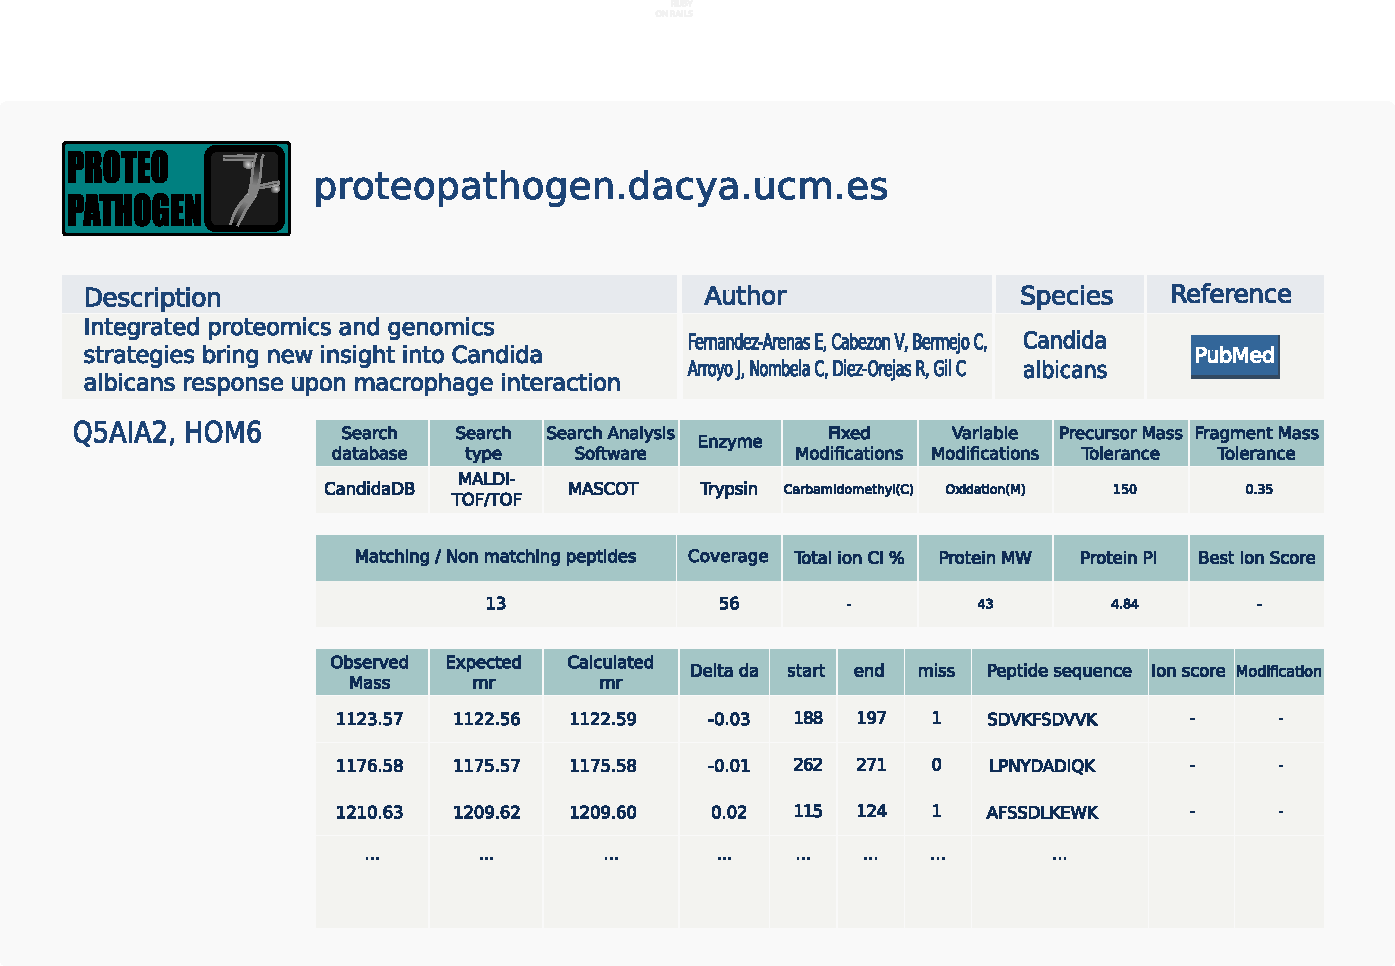
\includegraphics[width=1\textwidth]{Imagenes/Vectorial/graphical_abstract_Proteopathogen1}



\newpage

%\includepdf[pages=-,scale=.85,pagecommand={}]{Capitulos/Vialas_2009_Proteopathogen_Proteomics.pdf}
%\includepdf[pages=-,pagecommand={}]{Proteopathogen/Vialas_2009_Proteopathogen_Proteomics.pdf}


%\section*{Proteopathogen, a protein database for studying \mbox{\textit{Candida albicans}} - host interaction}

\chapter*{Abstract}

There exist, at present, public web repositories for management and storage of proteomic
data and also fungi-specific databases. None of them, however, is focused to the specific
research area of fungal pathogens and their interactions with the host, and contains
proteomics experimental data. In this context, we present Proteopathogen, a database
intended to compile proteomics experimental data and to facilitate storage and access to a
range of data which spans proteomics workflows from description of the experimental
approaches leading to sample preparation to MS settings and peptides supporting protein
identification. Proteopathogen is currently focused on \textit{Candida albicans} and its interaction
with macrophages; however, data from experiments concerning different pathogenic fungi
species and other mammalian cells may also be found suitable for inclusion into the database. 

Proteopathogen is publicly available at \href{http://proteopathogen.dacya.ucm.es}{http://proteopathogen.dacya.ucm.es}

\newpage{}

\textit{Candida albicans} is an opportunistic pathogenic fungus,
which can be found as a component of the usual flora in
human mucoses. Although it does not normally cause
disease in immunocompetent colonized hosts, in the case
of immunosuppressed patients \textit{Candida} cells can overproliferate
 and become pathogenic. Cells in yeast form (oval
cells) may produce hyphae, penetrate tissues and eventually
cause invasive candidiasis. At present, the frequency of this
fatal opportunistic mycosis continues to be distressing and,
unfortunately, solution is hindered by the reduced effectiveness
 and serious side effects of the few available drugs,
the appearance of antifungal-drug resistance, and the lack of
accurate and prompt diagnostic procedures \citep{Calderone2012}.

Addressing proteomic studies involving the way \textit{Candida}
interacts with immune cells is thus essential in order to
improve our comprehension of the process of infection and
represents the primary step of investigation that could lead
to future development of diagnosis methods, vaccines and
antifungal drugs \citep{Fernandez-Arenas2007, Martinez-Solano2006a, Pitarch2006, Pitarch2006a}.


Experimental techniques in proteomics have quickly
evolved in such a way that nowadays we have to deal with
vast amounts of complex data originated by the combination
of multi-dimensional separation techniques and MS analysis
 together with the bioinformatics software reports \citep{Monteoliva2004}.
Existing public repositories for management and storage of
proteomic data such as World 2-D PAGE \citep{Hoogland2008}, the Proteome
Database System for Microbial Research 2-D PAGE \citep{Pleissner2004}, or
PRIDE \citep{Martens2005}; and fungi-specific databases such as BioBase
MycoPathPD \citep{Csank2002}, Candida Genome Database (CGD) \citep{Arnaud2005}
or Candida DB \citep{Rossignol2008} are very popular and useful tools.
However, none of them deals with proteomic experimental
data related to the specific research area of fungal pathogens
and their interaction with the host. In this context,
we present Proteopathogen, a protein database, currently
focused on the \textit{\mbox{C. albicans}} - macrophage interaction
model - which enables a framework for the access and
submission of proteomic workflow data, from description of
the experimental approaches leading to sample preparation
to MS settings and identification - supporting peptides.
Through its interface web site, the database can easily be
queried to allow an efficient browsing through all the stored
data, improving the quality of eventual analysis of MS
results.

Regarding the compilation of information used to
populate the database, data from three different studies were
considered suitable to be present in Proteopathogen.
The first two correspond to publish works relating to
proteomics of the \textit{Candida} - macrophage interaction
\citep{Fernandez-Arenas2007, Martinez-Solano2006a}, where the former reports 
66 different \textit{\mbox{C. albicans}}
identified proteins and the latter, 38 murine macrophage
proteins. The third study represents an analysis of the
\textit{\mbox{C. albicans}} plasma membrane proteome \citep{Cabezon2009}. It compiles
a set of experiments aimed at extraction and identification of
membrane proteins and a set of experiments intended to
obtain enrichment in glycosylphosphatidylinositol-anchored
surface proteins, which have been reported to be involved in
cell wall biogenesis, cell-cell adhesion and interaction with
the host \citep{Plaine2008}.




\begin{table}[t]

\caption*{Table 1. Overview of the stored data in Proteopathogen as well as their published evidences.}

\renewcommand{\arraystretch}{2}
\footnotesize
\centering

\begin{tabular}{p{3cm} p{4cm} l p{2cm} }

\hline
References & Description of  \newline{} experimental approach & Species & \#Protein \newline{} identifications \\
\hline
\

\citep{Fernandez-Arenas2007} & \mbox{C. albicans} differentially expressed proteins after 3 h interaction with RAW 264.7 murine macrophages. 2-D silver-stained gel. MS/MS (MALDI/TOF-TOF) & \textit{\mbox{C. albicans}} & 66\\

\citep{Martinez-Solano2006a} & Proteins identified from cytoplasmic extracts of RAW 264.7 cells after 45 min interaction with \textit{C.albicans} & \textit{Mus musculus} & 38\\

\citep{Cabezon2009} & Identification of Glycosyl phosphatidil inositol (GPI)-anchored membrane proteins & \textit{C. albicans} & 292\\

 & Identification of membrane proteins &  & 1273\\

\end{tabular}
\end{table}
\addcontentsline{lot}{table}{Table 1}



In all cases, protein identifications lists are collected
together with the pertinent experimental context specified
by descriptions of the experimental approaches, MS settings
and peptides supporting identification for each of the
proteins (Table 1).

Along with the experimental information, and in order to
provide a deeper view of the data, complementary information
 is retrieved from public web repositories. In the
case of \textit{\mbox{C. albicans}} proteins, identifiers, synonyms, aminoacid
sequence of the translated open reading frame, \textit{Saccharomyces
cerevisiae} orthologs, Gene Ontology (GO) annotation, pathway
annotations and scientific literature references were obtained
from CGD \citep{Arnaud2005}, whereas in the case of murine macrophage
proteins, the equivalent information was obtained from
UniProt KnowledgeBase \citep{Uniprot2008} and the Mouse Genome Database
 \citep{Bult2008}. Additionally, pathways annotations were retrieved
from Kyoto Encyclopedia of Genes and Genomes (KEGG)
Pathway Database \citep{Kanehisa2007} and structure information from the
Protein Data Bank (PDB) \citep{Berman2000}.

\setcounter{chapter}{2}
\setcounter{figure}{0}

%\figura{Vectorial/proteopathogen1}{width=.99\textwidth}{fig:proteopathogen1}%
%{Search for \textit{C. albicans} ubiquinol-cytochrome-c reductase QCR2}



\begin{figure}[t]
\begin{center}
 \includegraphics[width=0.93\textwidth]%
				 {Imagenes/Vectorial/proteopathogen1}
\caption*{Figure 1. Use case: Search for \textit{\mbox{C. albicans}} ubiquinol-cytochrome-c
reductase QCR2. The different sections in the result comprise information
on protein description and identifiers, experiments in which it has been
identified, GO annotation, KEGG and CGD pathway annotation and 
structural information from PDB.}
\end{center}
\end{figure}
\addcontentsline{lof}{figure}{Figure 1}

Concerning the architecture of the software, the back-end
layer consists of a MySQL database managed by the web
application development framework Ruby on Rails that sets
up structure and relations of data, handles queries to the
database and displays the user web-based interface.

The experimental context is addressed in Proteopathogen
in a hierarchical manner, where a main general approach,
which may correspond to a published article, is characterized
 by a description or title, authors, target species and
Pubmed identifier when available; and experiments within
it, are in they turn, characterized by the description of the
particular experiment, the date when it was performed and
number of identified proteins.

Information on one particular protein is split into several
sections in Proteopathogen. Protein Basic Information
displays the UniProt accession number, description, species,
evidence for the existence, standard gene name, organism-
specific database identifiers, yeast orthologs for \textit{Candida}
proteins and human orthologs for mouse proteins and
sequence. The Section 2 lists experiments in which the
particular protein has been identified. Where available,
one or more of the following sections will be displayed
as well: the table entitled GO showing GO annotations
along with the pertinent scientific references, the KEGG
Pathways and CGD Pathways tables rendering annotations
from KEGG and CGD respectively, and PDB, a table
specifying structural information. Where no PDB identifiers
are found for \textit{\mbox{C. albicans}} proteins, \textit{S. cerevisiae} orthologs
are used instead, and similarly, when a PDB identifier
cannot be found for mouse proteins, the human ortholog
is used.

In all cases, proteins are unambiguously related to their
corresponding experiment, thus enabling a relation to the
data concerning experimental parameters of identification
and identification-supporting peptides. This data comprise,
on the one hand, common MS settings for all proteins
identified in the particular experiment, including search
database, MS type, analysis software, digestion enzyme,
fixed aminoacid modifications, variable modifications and
maximum allowed number of miscleavages; and on the
other hand, particular parameters and peptides list for each
protein, including number of matched peptides, score,
observed peptide mass, calculated peptide mass, start and
end coordinates, number of missed cleavages and the
sequence of the peptide.

The web interface to Proteopathogen offers multiple
ways to query the database. Through the Browse Experiments
search option, a list containing all sets of experimental
approaches is displayed. In its turn, one particular
experiment can be browsed through all the proteins
identified in it.

The Search form may be used in different manners.
Queries for one particular protein can be performed by
supplying one of the multiple supported identifiers, namely
standard gene names, \textit{Candida} feature name, Candida DB
identifiers, CGD identifiers, MGI identifiers and UniProt
accession numbers. Free text queries can be performed as
well, which will retrieve a list of proteins showing coincidences
 in the description field of the Proteopathogen
protein entry. As an additional feature, peptide sequences
can also be searched for retrieving in this case, proteins in
any experiment having the searched sequence in any of the
identification-supporting peptides. Wild characters (*)
and boolean operators are supported for free text queries
and for peptide sequence queries.

In order to enhance interactivity and collaboration
with users, a submission form is included in the web
interface to allow the upload of more proteomic experimental
 approaches as long as they concern the topics
addressed in Proteopathogen. Sequential steps request from
the user the following information: a description of the
experimental context, a related protein list, MS parameters
and identification-supporting peptides lists. These data are
subject to revision prior to eventual insertion into Proteo-
pathogen by the database curators. Besides, the whole relational
 database and the MS data reports are available for
download at the web site.

All the information that is retrievable from Proteo-
pathogen when queried for one particular protein is shown
in Fig. 1 for the specific case of ubiquinol-cytochrome-c
reductase QCR2 of \textit{\mbox{C. albicans}} which has been reported to
show antigenic properties in human \citep{Pitarch2004}.

The Protein Basic Information section displays the
Uniprot accession number, a brief description of the protein
as stated at CGD, evidence for its existence, standard gene
name, feature name, CGD and Candida Database identi-
fiers, yeast ortholog gene name, synonyms and sequence.

The Section 2 lists all the experiments in which QCR2
has been identified. All of them belong to the same general
approach aimed at purification of membrane proteins. In
every case, the corresponding links to the MS identification
parameters and supporting peptides are displayed as well.
This experimental data are shown in Fig. 1 for identification
of QCR2 in the experiment described as "Method D.
Douncer homogenizer protoplast breaking and 12-60%
sucrose gradient. LC-LTQ".

The section entitled GO annotations shows terms related
to the electron transport chain, but more interestingly, it
also shows an inferred from direct assay (IDA) annotation to
the term membrane fraction \citep{Insenser2006}, which fits to the fact that
the protein is identified in five of the methods aimed at
purification of membrane proteins.

KEGG Pathways table provides a link to the KEGG
Pathway entry for Oxidative phosphorylation, and provides
the feature to show in place the image corresponding to the
map from KEGG. CGD Pathways displays an analogous link
to the pathway entry at CGD that, in this case, is named
aerobic respiration (cyanide sensitive)- electron donors.

Finally, in the PDB section, there are four structure
images available along with links to the PDB entries,
corresponding to a cytochrome bc1 complex from \textit{S. cerevisiae}.
 Orthologs were used since no structure could be found
for the \textit{Candida} protein.

In conclusion, Proteopathogen represents, up to date, the
first public web-based repository for proteomics data related
to studies involving \textit{\mbox{C. albicans}} pathogenicity and its interaction
 with immune system cells in the host. Moreover, it
enables a framework for public access and submission of
this type of data and it is intended to be more actively
populated in the near future, including data from different
pathogenic fungi and mammalian cells, becoming a refer-
ence database in its field. Unlike other protein identification
databases, Proteopathogen is focused to a specific topic but,
at the same time, includes a wide range of data including
descriptions of the experimental contexts, information on
proteins such as GO and pathway annotations, structural
information and detailed MS parameters. Therefore,
Proteopathogen will contribute to save time and facilitate
analysis of proteomic workflow reports for researchers
interested in this area.

\section*{References}


\begin{itemize}[leftmargin=*]

\item[]{
Arnaud, M. B., Costanzo, M. C., Skrzypek, M. S., Binkley, G., Lane, C., Miyasato, S. R., and
Sherlock, G. (2005), The Candida Genome Database (CGD), a community resource for
\textit{Candida albicans} gene and protein information., Nucleic acids research, 33(Database issue), D358-63.
}

\item[]{
Berman, H. M., Westbrook, J., Feng, Z., Gilliland, G., Bhat, T. N., Weissig, H., Shindyalov, I. N.,
and Bourne, P. E. (2000), The Protein Data Bank., Nucleic acids research, 28(1), 235-42.
}

\item[]{
Bult, C. J., Eppig, J. T., Kadin, J. A., Richardson, J. E., and Blake, J. A. (2008), The Mouse
Genome Database (MGD): mouse biology and model systems., Nucleic acids research,
36(Database issue), D724-8.
}

\item[]{
Cabez�n, V., Llama-Palacios, A., Nombela, C., Monteoliva, L., and Gil, C. (2009), Analysis of
\textit{Candida albicans} plasma membrane proteome., Proteomics, 9(20), 4770-86.
}

\item[]{
Calderone, R. (2012), Candida and candidiasis. ASM Press, Washington DC.
}

\item[]{
Csank, C., Costanzo, M. C., Hirschman, J., Hodges, P., Kranz, J. E., Mangan, M., O�eill,
K., Robertson, L. S., Skrzypek, M. S., Brooks, J., and Garrels, J. I. (2002), Three yeast
proteome databases: YPD, PombePD, and CalPD (MycoPathPD)., Methods in enzymology,
350, 347-73.
}

\item[]{
Fern�ndez-Arenas, E., Cabez�n, V., Bermejo, C., Arroyo, J., Nombela, C., Diez-Orejas, R.,
and Gil, C. (2007), Integrated proteomics and genomics strategies bring new insight into
\textit{Candida albicans} response upon macrophage interaction, Molecular \& cellular proteomics
: MCP, 6(3), 460-478.
}

\item[]{
Hoogland, C., Mostaguir, K., Appel, R. D., and Lisacek, F. (2008), The World-2DPAGE 
Constellation to promote and publish gel-based proteomics data through the ExPASy server.,
Journal of proteomics, 71(2), 245-8.
}

\item[]{
Insenser, M., Nombela, C., Molero, G., and Gil, C. (2006), Proteomic analysis of detergent -
resistant membranes from Candida albicans., Proteomics, 6 Suppl 1, S74-81.
}

\item[]{
Kanehisa, M., Araki, M., Goto, S., Hattori, M., Hirakawa, M., Itoh, M., Katayama, T., 
Kawashima, S., Okuda, S., Tokimatsu, T., and Yamanishi, Y. (2007), KEGG for linking genomes to
life and the environment, Nucleic Acids Research, 36(Database), D480-D484.
}

\item[]{
Martens, L., Hermjakob, H., Jones, P., Adamski, M., Taylor, C., States, D., Gevaert, K., Van-
dekerckhove, J., and Apweiler, R. (2005), PRIDE: the proteomics identifications database.,
Proteomics, 5(13), 3537-45.
}

\item[]{
Mart�nez-Solano, L., Nombela, C., Molero, G., and Gil, C. (2006), Differential 
protein expression of murine macrophages upon interaction with \textit{Candida albicans}, Proteomics, 6 Suppl
1, S133-S144.
}

\item[]{
Monteoliva, L. and Albar, J. P. (2004), Differential proteomics: an overview of gel and non-gel
based approaches., Briefings in functional genomics \& proteomics, 3(3), 220-39.
}

\item[]{
Pitarch, A., Abian, J., Carrascal, M., S�nchez, M., Nombela, C., and Gil, C. (2004),
Proteomics-based identification of novel \textit{Candida albicans} antigens for diagnosis 
of systemic candidiasis in patients with underlying hematological malignancies.,
Proteomics, 4(10), 3084-106.
}

\item[]{
Pitarch, A., Nombela, C., and Gil, C. (2006a), \textit{Candida albicans} biology and pathogenicity:
insights from proteomics., Methods of biochemical analysis, 49, 285-330.
}

\item[]{
Pitarch, A., Nombela, C., and Gil, C. (2006b), Contributions of proteomics to diagnosis, treat-
ment, and prevention of candidiasis., Methods of biochemical analysis, 49, 331-61.
}

\item[]{
Plaine, A., Walker, L., Da Costa, G., Mora-Montes, H. M., McKinnon, A., Gow, N. A. R., 
Gaillardin, C., Munro, C. A., and Richard, M. L. (2008), Functional analysis of Candida albicans
GPI-anchored proteins: roles in cell wall integrity and caspofungin sensitivity., 
Fungal genetics and biology : FG \& B, 45(10), 1404-14.
}

\item[]{
Pleissner, K.-P., Eifert, T., Buettner, S., Schmidt, F., Boehme, M., Meyer, T. F., Kaufmann, S.
H. E., and Jungblut, P. R. (2004), Web-accessible proteome databases for microbial 
research., Proteomics, 4(5), 1305-13.
}

\item[]{
Rossignol, T., Lechat, P., Cuomo, C., Zeng, Q., Moszer, I., and D�nfert, C. (2008), 
CandidaDB: a multi-genome database for Candida species and related Saccharomycotina.,
Nucleic acids research, 36(Database issue), D557-61.
}

\item[]{
The Uniprot Consortium (2008), The universal protein resource (UniProt).,
Nucleic acids research, 36(Database issue), D190-5.
}

\end{itemize}




%~ \setBibFiles{proteopathogen1}
%~ 
%~ \def\ficherosBibliografia{}
%~ \newcommand{\setBibFiles}[1]{
%~ \def\ficherosBibliografia{#1}
%~ }
%~ 
%~ \begingroup
%~ \spanishdeactivate{~}
%~ \bibliographystyle{TeXiS/TeXiS}
%~ %\bibliographystyle{abbrv}
%~ \bibliography{\ficherosBibliografia}
%~ \endgroup
 %Paper Proteopathogen 1
%---------------------------------------------------------------------
%
%                          Cap�tulo 2
%
%---------------------------------------------------------------------


\chapter*{%
\href{http://www.sciencedirect.com/science/article/pii/S2212968515000112}{%
Proteopathogen2: A database and web tool to store and display  proteomics identification results in the mzIdentML standard%
}%
}
\addcontentsline{toc}{chapter}{Proteopathogen2: A database and web tool to store and display proteomics \\  identification results in the mzIdentML standard}
%\fancyhf{} % clear all header and footer fields

%Ojo, solo para la versi�n B5
\addtocontents{lof}{\protect\newpage} %Ojo, solo para la versi�n B5



\addcontentsline{lof}{chapter}{Proteopathogen2: A database and web tool to store and display  proteomics \\  identification results in the mzIdentML standard}
\addcontentsline{lot}{chapter}{Proteopathogen2: A database and web tool to store and display  proteomics \\  identification results in the mzIdentML standard}



%\renewcommand{\headrulewidth}{0pt}
\cabeceraEspecial{Proteopathogen2, adapted to mzIdentML}

\subsubsection*{Vital Vialas, Concha Gil}
\subsubsection*{EuPA Open Proteomics 2015, 8, 22-27}

\bigskip
\hfill
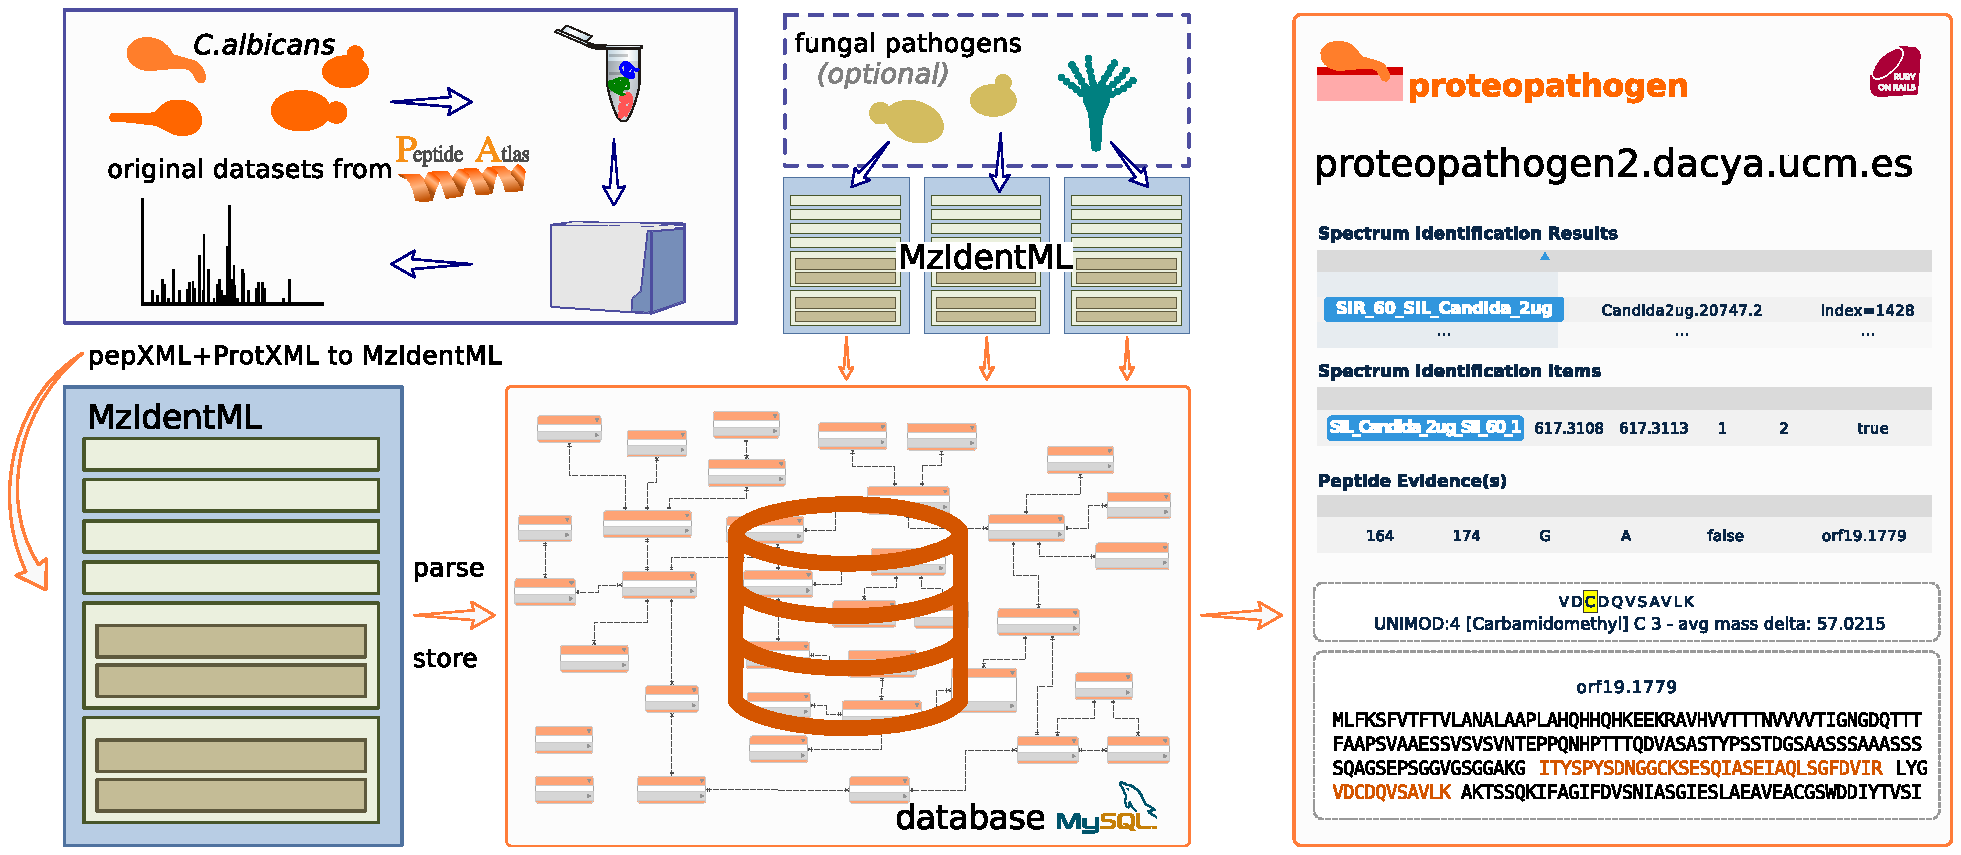
\includegraphics[width=1\textwidth]{Imagenes/Vectorial/graphical_abstract_proteopathogen2}



\newpage


%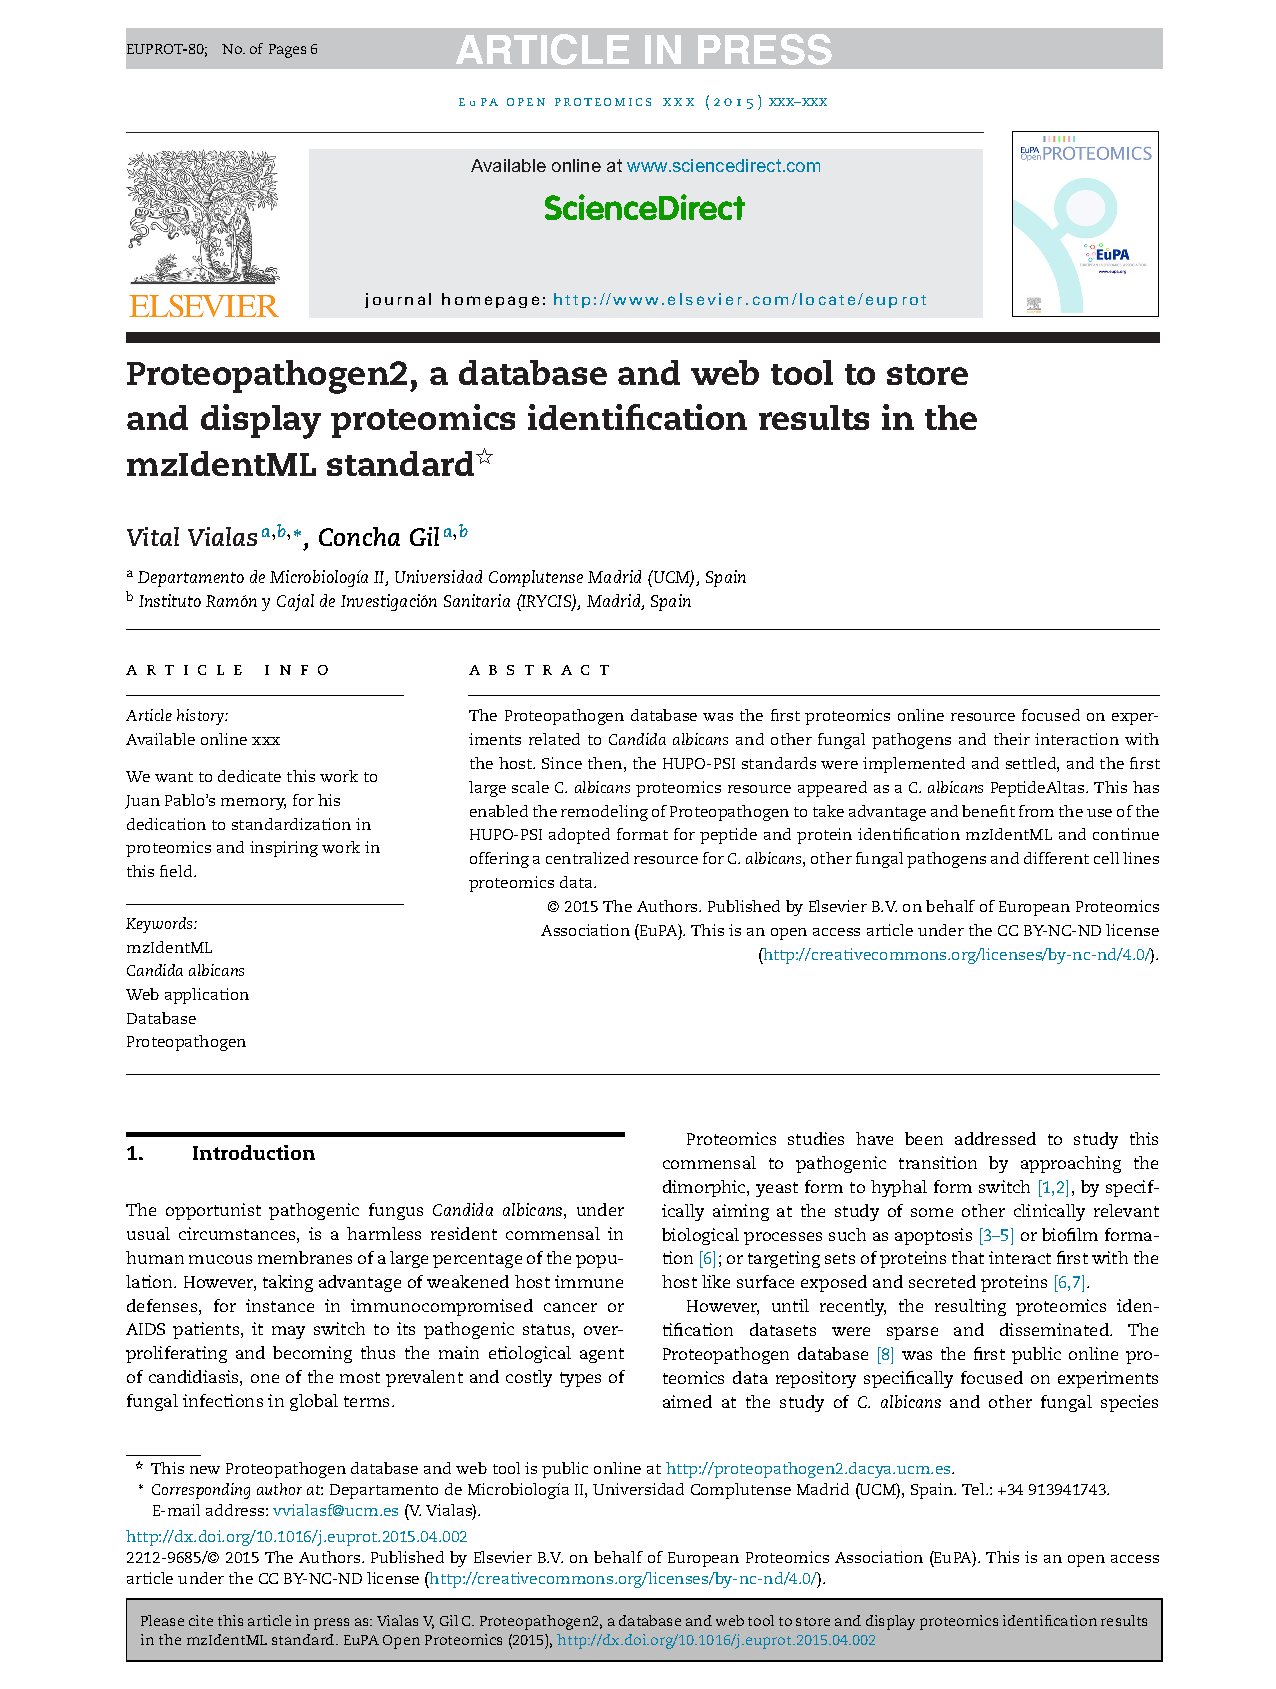
\includepdf[pages=-,pagecommand={}]{Proteopathogen/Vialas_2015_Proteopathogen2_EupaOpen.pdf}


\chapter*{Abstract}
The Proteopathogen database was the first proteomics online resource 
focused on experiments related to \textit{Candida albicans}
 and other fungal pathogens and their interaction with the host. 
 Since then, the HUPO-PSI standards were implemented and settled, and 
 the first large scale \textit{\mbox{C. albicans}} proteomics resource appeared 
 as a \textit{\mbox{C. albicans}} PeptideAltas. This has enabled the remodeling
 of Proteopathogen to take advantage and benefit from the use of the 
 HUPO-PSI adopted format for peptide and protein identification mzIdentML 
 and continue offering a centralized resource for \textit{\mbox{C. albicans}}, 
 other fungal pathogens and different cell lines proteomics data.

\newpage{}

\section*{Introduction}
\addcontentsline{toc}{section}{Introduction}

The opportunist pathogenic fungus \textit{Candida albicans}, under
usual circumstances, is a harmless resident commensal in
human mucous membranes of a large percentage of the population.
However, taking advantage of weakened host immune
defenses, for instance in immunocompromised cancer or
AIDS patients, it may switch to its pathogenic status, over-
proliferating and becoming thus the main etiological agent
of candidiasis, one of the most prevalent and costly types of
fungal infections in global terms.

Proteomics studies have been addressed to study this
commensal to pathogenic transition by approaching the
dimorphic, yeast form to hyphal form switch \citep{Monteoliva2010,Gow2011},
by specifically aiming at the study of some other clinically relevant
biological processes such as apoptosis \citep{Madeo2004, Fernandez-Arenas2007, Ramsdale2008} 
or biofilm formation \citep{Vialas2012};
or targeting sets of proteins that interact first with the
host like surface exposed and secreted proteins \citep{Vialas2012, Gil-Bona2015a}.

However, until recently, the resulting proteomics identification
 datasets were sparse and disseminated. The
Proteopathogen database \citep{Vialas2009b} was the first public online 
proteomics data repository specifically focused on experiments
aimed at the study of \textit{\mbox{C. albicans}} and other fungal species
pathogenic traits. Since no standard format for peptide and
protein identification results was available, Proteopathogen
was developed to compile and display identification lists in
different tabulated text formats depending on the software
used to generate and process the results.

At that time, the HUPO - Proteomics Standards Initiative
(PSI) already had a trajectory striving to highlight the importance 
of standardization and providing formats that would
comply with MIAPE (Minimum Information About a Proteomics
Experiment) guidelines as reviewed in ref \citep{Martinez-Bartolome2014}. 
Some \textit{de facto}
standard formats existed like mzXML and pepXML \citep{Deutsch2012}, but the
advent, years later, of the HUPO-PSI approved formats for mass
spectrometry output data \citep{Martens2011} and for identification results \citep{Jones2012}
among others, surfaced the efforts and claims by the community to finally
 adopt formats to facilitate data comparison,
exchange and verification. This also inspired and boosted the
development of an assortment of format conversion tools and
libraries \citep{Chambers2012, Griss2012} and stand-alone software for visualization of
the content of the files in standard formats \citep{Ghali2013} but, most
importantly for the purpose of this work, enabled the possibility
 for Proteopathogen to benefit from the mzIdentML adopted
standard for identification results, incorporating it as the input
data format and using it as inspiration for information display.

More recently, the most comprehensive, up to the current date, 
online \textit{\mbox{C. albicans}} proteomics data repository was
developed and integrated in PeptideAtlas \citep{Vialas2013}. These publicly
available \textit{\mbox{C. albicans}} results have been used to establish a new
version of Proteopathogen with a solid foundation.

In this background, we present here a revisited Proteopathogen
 database and web based tool adapted to read and
display peptide and protein identification data based upon
the mzIdentML format. It is the first online database specifically
 developed to map and store the contents of files in
mzIdentML, it has been initially populated with the \textit{\mbox{C. albicans}}
PeptideAtlas identification results and it is publicly accessible
at \href{http://proteopathogen2.dacya.ucm.es}{http://proteopathogen2.dacya.ucm.es}

\phantomsection{}
\section*{Materials and methods}
\addcontentsline{toc}{section}{Materials and methods}

The original identification result files were obtained from
PeptideAtlas repository datasets 
\href{ftp://ftp.peptideatlas.org/pub/PeptideAtlas/Repository/PAe001976/}{PAe001976},
\href{ftp://ftp.peptideatlas.org/pub/PeptideAtlas/Repository/PAe001977/}{PAe001977},
\href{ftp://ftp.peptideatlas.org/pub/PeptideAtlas/Repository/PAe001978/}{PAe001978}, 
\href{ftp://ftp.peptideatlas.org/pub/PeptideAtlas/Repository/PAe001979/}{PAe001979}, 
\href{ftp://ftp.peptideatlas.org/pub/PeptideAtlas/Repository/PAe001980/}{PAe001980}, 
\href{ftp://ftp.peptideatlas.org/pub/PeptideAtlas/Repository/PAe001981/}{PAe001981}, 
\href{ftp://ftp.peptideatlas.org/pub/PeptideAtlas/Repository/PAe001982/}{PAe001982},
\href{ftp://ftp.peptideatlas.org/pub/PeptideAtlas/Repository/PAe001983/}{PAe001983}, 
\href{ftp://ftp.peptideatlas.org/pub/PeptideAtlas/Repository/PAe001984/}{PAe001984}, 
\href{ftp://ftp.peptideatlas.org/pub/PeptideAtlas/Repository/PAe001985/}{PAe001985}, 
\href{ftp://ftp.peptideatlas.org/pub/PeptideAtlas/Repository/PAe001986/}{PAe001986}, 
\href{ftp://ftp.peptideatlas.org/pub/PeptideAtlas/Repository/PAe001987/}{PAe001987},
\href{ftp://ftp.peptideatlas.org/pub/PeptideAtlas/Repository/PAe001988/}{PAe001988}, 
\href{ftp://ftp.peptideatlas.org/pub/PeptideAtlas/Repository/PAe001989/}{PAe001989}, 
\newline
\href{ftp://ftp.peptideatlas.org/pub/PeptideAtlas/Repository/PAe002110/}{PAe002110}, and 
\href{ftp://ftp.peptideatlas.org/pub/PeptideAtlas/Repository/PAe002111/}{PAe002111}.

As described in Ref. \citep{Vialas2013} the data sets come from a range
of experiments including yeast to hypha transition assays,
membrane protein extractions and a set of phosphoprotein
enrichment approaches. In all cases, cells from the clinical isolates
 SC5314 were grown in YPD medium. For obtaining cells
in hyphal form, either heat-inactivated fetal bovine serum or
Lee medium pH 6.7 was used. As for the mass spectrometry,
spectra were acquired in different set ups and platforms in a
data-dependent manner. A summary of the experiments set
ups and conditions is shown in Table 1.

\begin{table}[t]
\caption*{Table 1. Summary of experiments, MS output files, instrument and PeptideAtlas datasets.}
\renewcommand{\arraystretch}{2}
\footnotesize
\centering

\begin{tabular}{p{3cm} cp{2cm} p{2cm} p{2cm} }

\hline
Type of dataset & Number of \newline{} MS output files & Instrument & PeptideAtlas \newline{} datasets \\
\hline

\textit{Candida albicans} culture with SILAC labelling, digested protein extracts enriched in \newline phosphopeptides IMAC/TiO2 & 57 & Orbitrap XL, \newline{} Orbitrap Velos &
\href{ftp://ftp.peptideatlas.org/pub/PeptideAtlas/Repository/PAe001976/}{PAe001976},
\href{ftp://ftp.peptideatlas.org/pub/PeptideAtlas/Repository/PAe001977/}{PAe001977},
\href{ftp://ftp.peptideatlas.org/pub/PeptideAtlas/Repository/PAe001978/}{PAe001978}, 
\href{ftp://ftp.peptideatlas.org/pub/PeptideAtlas/Repository/PAe001979/}{PAe001979}, 
\href{ftp://ftp.peptideatlas.org/pub/PeptideAtlas/Repository/PAe001980/}{PAe001980}, 
\href{ftp://ftp.peptideatlas.org/pub/PeptideAtlas/Repository/PAe001984/}{PAe001984}, 
\href{ftp://ftp.peptideatlas.org/pub/PeptideAtlas/Repository/PAe001985/}{PAe001985}, 
\href{ftp://ftp.peptideatlas.org/pub/PeptideAtlas/Repository/PAe001986/}{PAe001986}, 
\href{ftp://ftp.peptideatlas.org/pub/PeptideAtlas/Repository/PAe001987/}{PAe001987},
\href{ftp://ftp.peptideatlas.org/pub/PeptideAtlas/Repository/PAe001988/}{PAe001988}, 
\href{ftp://ftp.peptideatlas.org/pub/PeptideAtlas/Repository/PAe001989/}{PAe001989} \\

\textit{Candida albicans} total protein extract, 2 Triple-TOF runs, 2ug and 4ug & 2 & Triple-TOF & 
\href{ftp://ftp.peptideatlas.org/pub/PeptideAtlas/Repository/PAe001983/}{PAe001983}  \\

Hyphal form and yeast form total protein extracts & 8 & Orbitrap Velos &
\href{ftp://ftp.peptideatlas.org/pub/PeptideAtlas/Repository/PAe002110/}{PAe002110}, 
\href{ftp://ftp.peptideatlas.org/pub/PeptideAtlas/Repository/PAe002111/}{PAe002111}\\

LTQ membrane proteins \newline \citep{Cabezon2009} & 3 & LTQ &  
\href{ftp://ftp.peptideatlas.org/pub/PeptideAtlas/Repository/PAe001981/}{PAe001981}\\

LTQ proteins from acidic subproteome \citep{Monteoliva2010} & 8 & LTQ & 
\href{ftp://ftp.peptideatlas.org/pub/PeptideAtlas/Repository/PAe001982/}{PAe001982}\\

\end{tabular}
\end{table}
\addcontentsline{lot}{table}{Table 1}


Consistently with the PeptideAtlas project principles, the
MS output files were processed through the Trans Proteomic
Pipeline. The steps involved, first, sequence database searching
 using X! Tandem with k-score \citep{MacLean2006} and a custom sequence
database obtained from Candida Genome Database \citep{Costanzo2006a} with
appended decoy counterparts and common contaminants for
peptide-to-spectrum matching and FDR assessment. Then
the post-processing validation tools PeptideProphet \citep{Choi2008}, 
ProteinProphet \citep{Nesvizhskii2003}
and iProphet \citep{Shteynberg2011} provided filtered lists of peptides
and proteins with high probabilities. And finally FDR was computed for
 different probability thresholds.

Each of the PeptideAtlas repository datasets consists on
the MS output spectra files and a set of pepXML and protXML
files with lists of high confidence peptide and proteins respectively. 
These were combined, independently for each dataset,
by means of a custom script written in the Ruby scripting language
 (available in supplemental data) to create mzIdentML
files (mzIdentML version 1.1.0) with the merged information.
In order to check the files were generated correctly and ensure
data quality they were all validated (semantic and MIAPE-
compliant validation) with mzidValidator \citep{Ghali2013}.

A completely new MySQL relational database was implemented \textit{ad hoc}
 to map elements in the mzIdentML files as
depicted in Fig. 1 (schema available in supplemental data).
Then, using the Ruby scripting language (version 2.0.0) and
the Rails web application development framework (version
4.0.0) a script was created to parse the data in the mzIdentML
files, store the relevant elements in the corresponding tables
(available in supplemental data) and eventually create the web
application to display the data.



\phantomsection{}
\section*{Results and discussion}
\addcontentsline{toc}{section}{Results and discussion}


A total number of sixteen mzIdentML files, corresponding to
each of the PeptideAtlas repository datasets, grouped into
five different experiments were compiled and used to initially
 populate the Proteopathogen database. These account
for approximately 22,000 distinct peptides and 2600 different proteins
 that can be queried and viewed through the web
interface.

\begin{figure}[t]
\begin{center}
 \includegraphics[width=0.70\textwidth]%
				 {Imagenes/Vectorial/proteopathogen2_figure1}
\caption*{Figure 1. mzIdentML to database mapping. The MySQL schema was 
specifically designed to accommodate elements from the mzIdentML format.
Figure shows the one-to-many relationship between the 
<SpectrumIdentificationResult> and
<SpectrumIdentificationItem> elements.}
\end{center}
\end{figure}
\addcontentsline{lof}{figure}{Figure 1}


Precisely, a stringent FDR cut-off at the PSM level set at
0.005, yields 21,883 peptides with 0.0024 FDR (peptide level)
and 2577 proteins with 0.0170 FDR (protein level) as computed
 with Mayu, a software specifically designed to estimate
accurate protein level error rates in large datasets \citep{Reiter2009} (see
supplemental Table 1).

The mzIdentML contents can be browsed for each file in
Proteopathogen in a means inspired by the structure in the
format, particularly that under the <AnalysisData> element
containing the datasets generated by the analyses. That is, for
each mzIdentML file, shown in its experimental context, a user
can select either the spectrum identification information (corresponding
 to the <SpectrumIdentification> element) and view its
related information, the search protocol, search database and
the list of every peptide to spectrum assignment; or the protein detection
 (corresponding to the <ProteinDetection> element)
showing the list of peptides grouped into the inferred original
proteins (Fig. 2).


Notably, the information Proteopathogen displays will
depend on how complete the original mzIdentML files are.
For instance, for files including the optional <Fragmentation>
element under <SpectrumIdentificationItem>, Proteopathogen
will display an annotated and interactive MS/MS spectrum. In
addition, the optional <cvParam> and <userParam> elements,
that describe and annotate with controlled vocabularies
and user-defined information respectively different elements
throughout the file, might be more or less profuse depending
on the software that created them.


In addition to browsing through the contents of the stored
mzIdentML files, Proteopathogen implements a query system
yielding global results. That is, for a specific queried protein
 name, as found in the <ProteinDetectionHypothesis> name
attribute, the search results display all the distinct peptide
sequences found mapped into the protein sequence, regardless
 of the experiment in which they were identified, and the
supporting spectra for each peptide sequence, while keeping
track of the original <SpectrumIdentification> and mzIdentML
file. A peptide sequence may also be searched, obtaining, when
found, the corresponding protein, or group of proteins, and the
set of supporting spectra, again in global scope.

\begin{figure}[t]
\begin{center}
 \includegraphics[width=0.86\textwidth]%
				 {Imagenes/Vectorial/proteopathogen2_figure2}
\caption*{Figure 2. Information displayed in the web interface. 
Proteopathogen displays two main sets of information for the selected
mzIdentML file. The spectrum identification section shows how for each
spectrum there is a list of possible identification results, each 
having its peptide evidence, \textit{i.e.} a sequence at a particular
position in a protein sequence. The particular selected peptide is shown
in its protein context in the protein detection section, which displays 
the complete list of the inferred proteins for the selected mzIdentML 
file with links to Candida Genome Database (CGD).}
\end{center}
\end{figure}
\addcontentsline{lof}{figure}{Figure 2}

The use of the Ruby scripting language, unlike other compiled
 languages (Java, C/C++) that are commonly used in other
software used to visualize proteomics file formats, enables a
quick, easy to implement, flexible manner of parsing complex
XML files, and creation and manipulation of objects that have
to be stored in a very precise order in a database. In addition,
 the argument of speed in computationally intensive tasks
in favor of compiled languages is getting blurry nowadays
with the array of xml parsing libraries that are continuously
developed and improved for scripting languages. The type of
solution implemented in Proteopathogen is a DOM (Document
Object Model) parser, that creates an in-memory tree representation
 of the whole XML hierarchy. Arguably, a parser of
the type SAX (Simple API for XML parsing) would perform better
 in terms of speed for large files but as trade-off, leaping
back and forth in search of cross-referenced elements, as is
the case in mzIdentML, would be difficult or even impossible to implement. 
Nevertheless, future work in the direction
of a SAX implementation of the parser and a comparison in
performance with respect to the current one, would be of great
interest.

Proteopathogen will greatly benefit from the adoption of
mzIdentML as input data format. Any proteomics experiment
on \textit{\mbox{C. albicans}}, or any fungal pathogen-host interaction, as long
as they are provided in valid (semantically valid and MIAPE-
compliant) mzIdentML (version 1.1.0), will be welcome to be
integrated in the database. To that purpose, users provided
with login credentials may submit their files either through a
simple upload form in the web application or transfer them
using a specifically set up FTP server. Finally, the Rails framework
 for web application development will take care of any
scalability issues with ease and allow for any kind of visualization improvements.

\phantomsection{}
\section*{Conclusions}
\addcontentsline{toc}{section}{Conclusions}

The Proteopathogen web application and database has been
completely rebuilt to accommodate and display \textit{C. albicans}, or
any fungal pathogen for that matter, proteomics identification
results in the HUPO-PSI adopted format for peptide and protein
identification mzIdentML. This makes it the first public
online database specifically designed to store the information
contained in these types of files and display its contents
following an analogous structure.


%\phantomsection{}
\section*{Acknowledgements}
This work has been financially supported by project
BIO2012-31767 Ministerio de Econom�a y Competitividad,
Spain, PROPMT (S2010/BMD-2414) from the Comunidad
Aut�noma de Madrid, REIPI, Spanish Network for the
Research in Infectious Diseases (RD12/0015/0004), and PRB2
(PT13/0001/0004) from the ISCIII. VV held a research contract
associated to project BIO2012-31767. The authors are grate-
ful to Daniel Tabas-Madrid and Alberto Pascual Montano from
CNB-CSIC for outstanding support and assistance in setting
up the web application.


\subsubsection*{Supplementary data}
Supplementary data associated with this article can be found,
in the online version, at \linebreak doi:10.1016/j.euprot.2015.04.002 \href{http://dx.doi.org/10.1016/j.jprot.2015.10.019}{http://dx.doi.org/10.1016/j.jprot.2015.10.019}



\phantomsection{}
\section*{References}
\addcontentsline{toc}{section}{References}

\begin{itemize}[leftmargin=*]

\item[]{
Cabez�n, V., Llama-Palacios, A., Nombela, C., Monteoliva, L., and Gil, C. (2009), Analysis of
\textit{Candida albicans} plasma membrane proteome., Proteomics, 9(20), 4770-86.
}

\item[]{
Chambers, M. C., Maclean, B., Burke, R., Amodei, D., Ruderman, D. L., Neumann, S., Gatto,
L., Fischer, B., Pratt, B., Egertson, J., Hoff, K., Kessner, D., Tasman, N., Shulman, N., 
Frewen, B., Baker, T. A., Brusniak, M.-Y., Paulse, C., Creasy, D., Flashner, L., Kani, K., Moulding,
C., Seymour, S. L., Nuwaysir, L. M., Lefebvre, B., Kuhlmann, F., Roark, J., Rainer, P., Detlev,
S., Hemenway, T., Huhmer, A., Langridge, J., Connolly, B., Chadick, T., Holly, K., Eckels,
J., Deutsch, E. W., Moritz, R. L., Katz, J. E., Agus, D. B., MacCoss, M., Tabb, D. L., and
Mallick, P. (2012), A cross-platform toolkit for mass spectrometry and proteomics., Nature
biotechnology, 30(10), 918-20
}

\item[]{
Choi, H. and Nesvizhskii, A. I. (2008), Semisupervised model-based validation of peptide 
identifications in mass spectrometry-based proteomics., Journal of proteome research, 7(1),
254-65.
}

\item[]{
Costanzo, M. C., Arnaud, M. B., Skrzypek, M. S., Binkley, G., Lane, C., Miyasato, S. R., and
Sherlock, G. (2006), The Candida Genome Database: facilitating research on 
\textit{Candida albicans} molecular biology., FEMS yeast research, 6(5), 671-84.
}

\item[]{
Deutsch, E. (2012), File formats commonly used in mass spectrometry proteomics, Molecular
\& Cellular Proteomics, 11(12), 1612-1621.
}

\item[]{
Fern�ndez-Arenas, E., Cabez�n, V., Bermejo, C., Arroyo, J., Nombela, C., Diez-Orejas, R.,
and Gil, C. (2007), Integrated proteomics and genomics strategies bring new insight into
\textit{Candida albicans} response upon macrophage interaction., Molecular \& cellular proteomics
: MCP, 6(3), 460-478.
}

\item[]{
Ghali, F., Krishna, R., Lukasse, P., Mart�nez-Bartolom�, S., Reisinger, F., Hermjakob, H., 
Vizca�no, J. A., and Jones, A. R. (2013), Tools (Viewer, Library and Validator) that facilitate use
of the peptide and protein identification standard format, termed mzIdentML., Molecular \&
cellular proteomics : MCP, 12(11), 3026-35.
}

\item[]{
Gil-Bona, A., Llama-Palacios, A., Parra, C. M., Vivanco, F., Nombela, C., Monteoliva, L., and
Gil, C. (2014), Proteomics unravels extracellular vesicles as carriers of classical cytoplasmic
proteins in Candida albicans., Journal of proteome research, 14(1), 142-53.
}

\item[]{
Gow, N. and van de Veerdonk, F. (2011), \textit{Candida albicans} morphogenesis and host defence:
discriminating invasion from colonization, Nature Reviews, 10(2), 112-122.
}

\item[]{
Griss, J., Reisinger, F., Hermjakob, H., and Vizca�no, J. A. (2012), jmzReader: A Java 
parser library to process and visualize multiple text and XML-based mass spectrometry data
formats., Proteomics, 12(6), 795-8.
}

\item[]{
Jones, A. R., Eisenacher, M., Mayer, G., Kohlbacher, O., Siepen, J., Hubbard, S. J., Selley,
J. N., Searle, B. C., Shofstahl, J., Seymour, S. L., Julian, R., Binz, P.-A., Deutsch, E. W.,
Hermjakob, H., Reisinger, F., Griss, J., Vizca�no, J. A., Chambers, M., Pizarro, A., and
Creasy, D. (2012), The mzIdentML data standard for mass spectrometry-based proteomics
results., Molecular \& cellular proteomics : MCP, 11(7), M111.014381.
}

\item[]{
Madeo, F., Herker, E., and Wissing, S. (2004), Apoptosis in yeast, Current opinion in 
microbiology, 7(6), 655-660
}

\item[]{
MacLean, B., Eng, J., Beavis, R., and McIntosh, M. (2006), General framework for developing
and evaluating database scoring algorithms using the TANDEM search engine, Bioinformatics, 22(22), 2830-2832.
}

\item[]{
Martens, L., Chambers, M., Sturm, M., Kessner, D., Levander, F., Shofstahl, J., Tang, W. H.,
R�mpp, A., Neumann, S., Pizarro, A. D., Montecchi-Palazzi, L., Tasman, N., Coleman, M.,
Reisinger, F., Souda, P., Hermjakob, H., Binz, P.-A., and Deutsch, E. W. (2011), mzML-a
community standard for mass spectrometry data., Molecular \& cellular proteomics : MCP,
10(1), R110.000133.
}

\item[]{
Mart�nez-Bartolom�, S., Binz, P.-A., and Albar, J. P. (2014), The Minimal Information about
a Proteomics Experiment (MIAPE) from the Proteomics Standards Initiative., Methods in
molecular biology (Clifton, N.J.), 1072, 765-80.
}

\item[]{
Monteoliva, L., Martinez-Lopez, R., Pitarch, A., Hernaez, M. L., Serna, A., Nombela, C., Albar,
J. P., and Gil, C. (2011), Quantitative proteome and acidic subproteome profiling of Candida
albicans yeast-to-hypha transition, Journal of Proteome Research, 10(2), 502-517.
}

\item[]{
Nesvizhskii, A. I., Keller, A., Kolker, E., and Aebersold, R. (2003), A statistical model for 
identifying proteins by tandem mass spectrometry., Analytical chemistry, 75(17), 4646-58.
}


\item[]{
Ramsdale, M. (2008), Programmed cell death in pathogenic fungi, Biochimica et Biophysica
Acta (BBA)-Molecular Cell Research, 1783(7), 1369-1380.
}

\item[]{
Reiter, L., Claassen, M., Schrimpf, S. S. P., Jovanovic, M., Schmidt, A., Buhmann, J. M., 
Hengartner, M. O., and Aebersold, R. (2009), Protein identification false discovery rates for very
large proteomics data sets generated by tandem mass spectrometry, Molecular \& Cellular
Proteomics, 8(11), 2405-2417.
}

\item[]{
Shteynberg, D., Deutsch, E. W., Lam, H., Eng, J. K., Sun, Z., Tasman, N., Mendoza, L., Moritz,
R. L., Aebersold, R., and Nesvizhskii, a. I. (2011), iProphet: Multi-level Integrative Analysis
of Shotgun Proteomic Data Improves Peptide and Protein Identification Rates and Error
Estimates, Molecular \& Cellular Proteomics, 10(12), M111.007690-M111.007690.
}

\item[]{
Vial�s, V., Nogales-Cadenas, R., Nombela, C., Pascual-Montano, A., and Gil, C. (2009), 
Proteopathogen, a protein database for studying Candida albicans-host interaction., 
Proteomics, 9(20), 4664-8.
}

\item[]{
Vial�s, V., Perumal, P., Gutierrez, D., Xim�nez-Emb�n, P., Nombela, C., Gil, C., and Chaffin,
W. L. (2012), Cell surface shaving of \textit{Candida albicans} biofilms, hyphae and yeast form
cells., Proteomics, 12(14), 2331-2339.
}

\item[]{
Vialas, V., Sun, Z., Loureiro Y Penha, C. V., Carrascal, M., Abi�n, J., Monteoliva, L., Deutsch,
E. W., Aebersold, R., Moritz, R. L., and Gil, C. (2013), A \textit{Candida albicans} PeptideAtlas.,
Journal of proteomics, 97, 62-8.
}






\end{itemize}
 %Proteopathogen 2

%---------------------------------------------------------------------
%
%                          Parte PeptideAtlas
%
%---------------------------------------------------------------------
%

%Solo para A4:
\addtocontents{toc}{\protect\newpage}

\partTitle{\sc{Creaci�n de un PeptideAtlas de \mbox{\textit{Candida albicans}}}}



\partDesc{ 
\begin{FraseCelebre}
\begin{Frase}
What evidence should satisfy you? 
Evidence that is publicly recorded and properly analysed
\end{Frase}
\begin{Fuente}
Richard Dawkins\\
Unweaving the rainbow
\end{Fuente}
\end{FraseCelebre}
}


%\partBackText{}

\makepart


 %Creacion de un PeptideAtlas de C.albicans
%---------------------------------------------------------------------
%
%                          PeptideAtlas 1
%
%---------------------------------------------------------------------

\begin{otherlanguage}{british}

\chapter*{\href{http://www.ncbi.nlm.nih.gov/pubmed/23811049}{A \textit{Candida albicans} PeptideAtlas}}
\addcontentsline{toc}{chapter}{A \textit{Candida albicans} PeptideAtlas}
%\cabeceraEspecial{A \textit{\textit{Candida albicans}} PeptideAtlas}
\addcontentsline{lof}{chapter}{A \textit{Candida albicans} PeptideAtlas}
\addcontentsline{lot}{chapter}{A \textit{Candida albicans} PeptideAtlas}


%\renewcommand{\headrulewidth}{0pt}
\cabeceraEspecial{A \textit{Candida albicans} PeptideAtlas}

\subsubsection*{Vital Vialas, Zhi Sun, Carla Ver\'onica Loureiro y Penha, Montserrat Carrascal, Joaqu\'in Abi\'an, Luc\'ia Monteoliva, Eric W. Deutsch, Ruedi Aebersold, Robert L. Moritz, Concha Gil}
\subsubsection*{Journal of Proteomics 2014, 97, 62-68}

%\subsubsection*{\href{http://www.ncbi.nlm.nih.gov/pubmed/23811049}{PMID: 23811049}}

\bigskip
\hfill
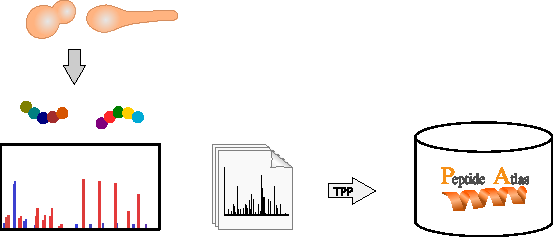
\includegraphics[width=1\textwidth]{Imagenes/Vectorial/graphical_abstract_PeptideAtlas1}



\newpage


%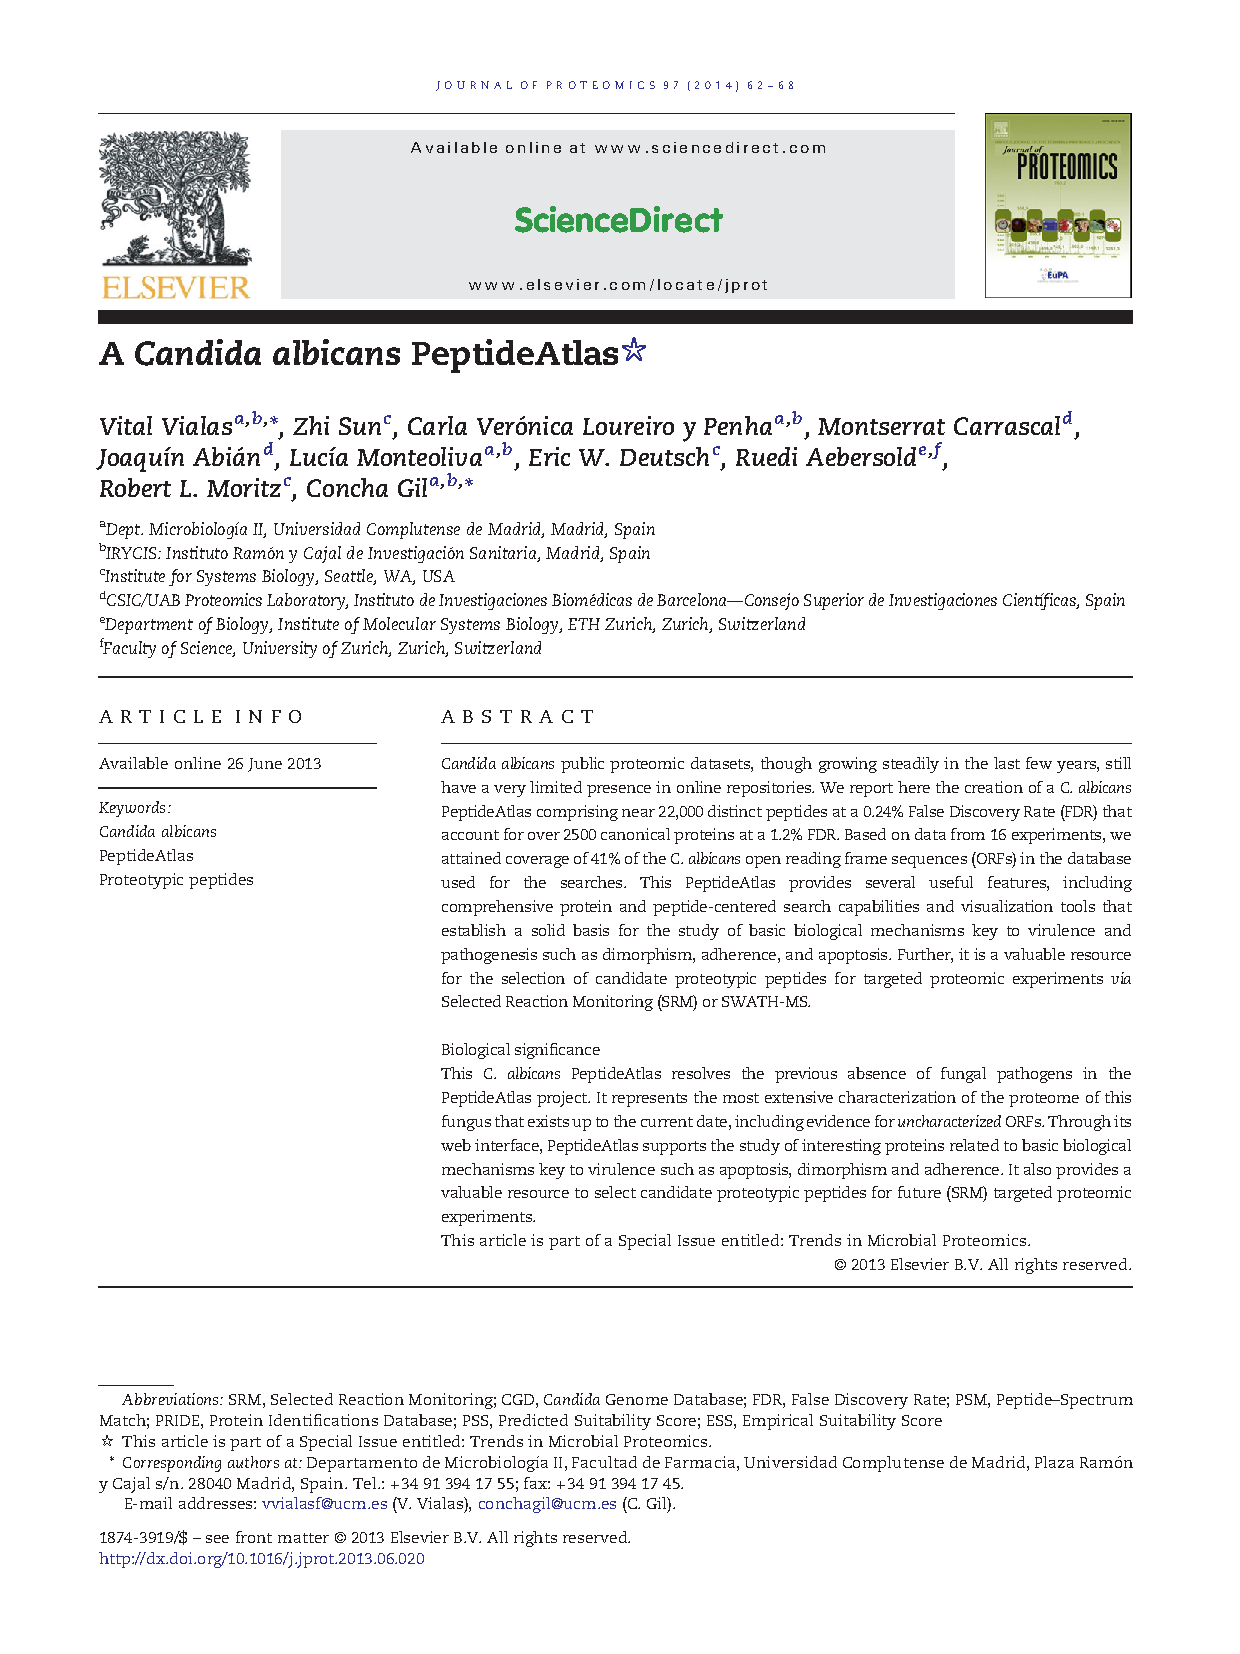
\includepdf[pages=-,scale=.8,pagecommand={}]{PeptideAtlas/Vialas_2013_PeptideAtlas_JProteomics.pdf}
%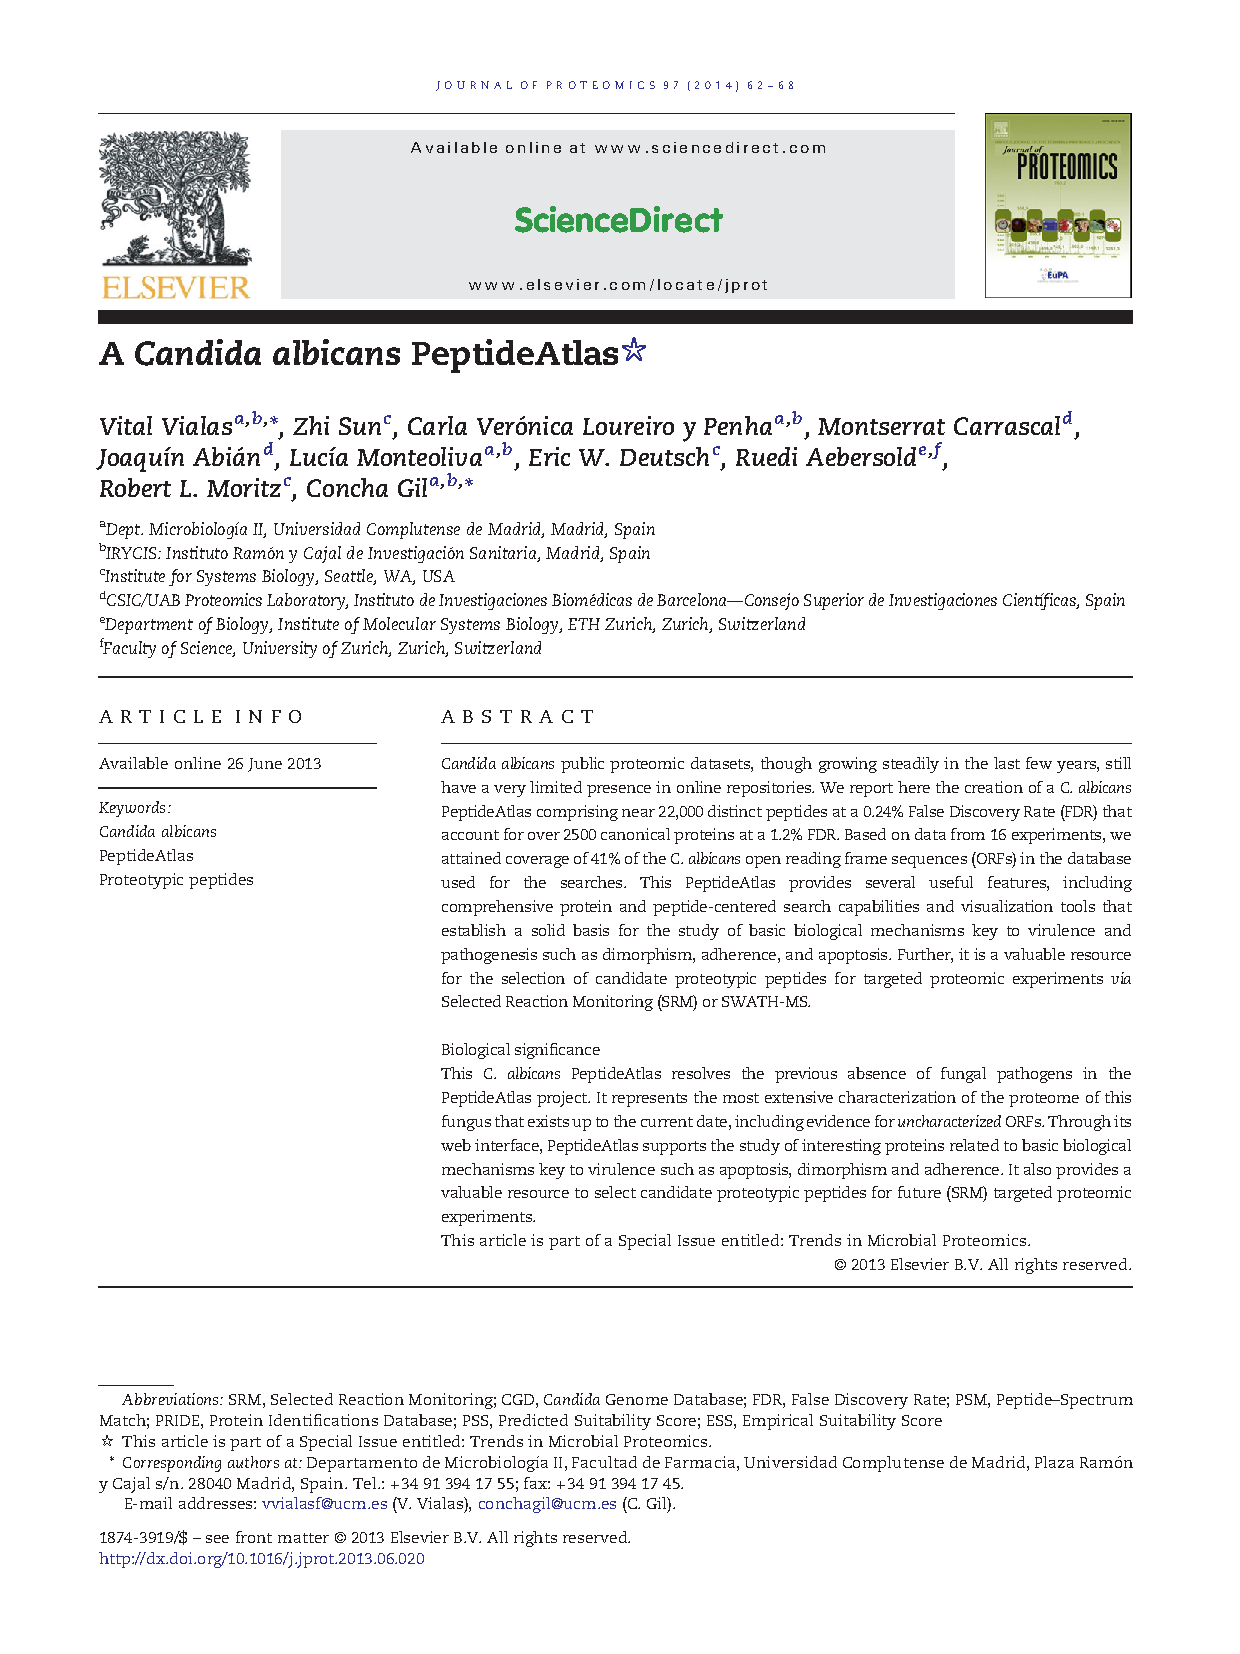
\includepdf[pages=-,pagecommand={}]{PeptideAtlas/Vialas_2013_PeptideAtlas_JProteomics.pdf}



\chapter*{Abstract}
\textit{Candida albicans} public proteomic datasets, though growing
 steadily in the last few years, still have a very limited presence in
 online repositories. We report here the creation of a \textit{\mbox{C. albicans}} PeptideAtlas
 comprising near 22,000 distinct peptides at a 0.24\% False Discovery
 Rate (FDR) that account for over 2500 canonical proteins at a 1.2\% FDR.
 Based on data from 16 experiments, we attained coverage of 41\% of the 
 \textit{\mbox{C. albicans}} open reading frame sequences (ORFs) in the database used 
 for the searches. This PeptideAtlas provides several useful features, 
 including comprehensive protein and peptide-centered search 
 capabilities and visualization tools that establish a solid basis for 
 the study of basic biological mechanisms key to virulence and 
 pathogenesis such as dimorphism, adherence, and apoptosis. 
 Further, it is a valuable resource for the selection of candidate 
 proteotypic peptides for targeted proteomic experiments via Selected
 Reaction Monitoring (SRM) or SWATH-MS

\subsection*{Biological Significance}
This \textit{\mbox{C. albicans}} PeptideAtlas resolves the previous absence of fungal 
pathogens in the PeptideAtlas project. It represents the most extensive
characterization of the proteome of this fungus that exists up to the 
current date, including evidence for uncharacterized ORFs. Through its 
web interface, \mbox{PeptideAtlas} supports the study of interesting proteins 
related to basic biological mechanisms key to virulence such as 
apoptosis, dimorphism and adherence. It also provides a valuable 
resource to select candidate proteotypic peptides for future (SRM) 
targeted proteomic experiments. 
This article is part of a Special Issue entitled: Trends in Microbial Proteomics.

\newpage


\phantomsection{}
\section*{Introduction}
\addcontentsline{toc}{section}{Introduction}

\textit{Candida albicans} is a fungus of great clinical importance. In
addition to asymptomatically colonizing mucous membranes
as a commensal in a large percentage of the population, it
may cause severe opportunistic infections in specific cases
such as patients with weakened immune defenses, a common
circumstance in cancer and AIDS patients. \textit{\mbox{C. albicans}} infections
are also a threat to patients in post-surgical situations and
intensive care unit stays. In this respect, invasive candidiasis
remains nowadays one of the major types of nosocomial
infections and a challenge in terms of economical and health
costs \citep{Wisplinghoff2004, Moran2010, Tong2008}.
From the perspective of proteomics, recent studies
have provided new insights into the \textit{\mbox{C. albicans}} biology and
suggested new clinical biomarker candidates for diagnosis and
prognosis of invasive candidiasis \citep{Pitarch2006, Pitarch2006a,
Fernandez-Arenas2007, Pitarch2011}.

However, the clinical relevance of this organism is not
reflected in the number of large-scale publicly available proteo-
mics resources. Up to the current date, the PRIDE \citep{Vizcaino2013} database
includes only 15 experiments accounting for 1786 identified
proteins. The more \textit{\mbox{C. albicans}}-focused Proteopathogen database
\citep{Vialas2009b} comprises several hundred protein identifications including
data from gel based proteomics, and other major proteomic
online resources such as the Global Proteome Machine Database 
(GPMDB \citep{Craig2004}) or Tranche \citep{Smith2011} contain no \textit{\mbox{C. albicans}} data
whatsoever.

As for the genomic data, according to \textit{Candida} Genome
Database (CGD), currently the most comprehensively annotated
\textit{\mbox{C. albicans}} sequence repository \citep{Costanzo2006a}, the \textit{\mbox{C. albicans}} genome
contains 6215 ORFs (as of May 28, 2013), out of which 1497 are
annotated as verified, i.e. representing genes for which there is
empirical evidence that the ORF actually encodes a functionally
characterized protein. In contrast, 4566 ORFs are termed
uncharacterized, indicating that there exists no conclusive evidence 
for the existence of a protein product. This data implies
that most part of the predicted proteome, over 70\% of the ORFs, is
still unknown or has not been properly annotated yet. An
extensive characterization of the \textit{\mbox{C. albicans}} proteome will
therefore be of great value to increase our knowledge in proteins
involved in mechanisms of virulence and infection and, thus
serves as a basis to design strategies for diagnosis, vaccination
and treatment of invasive candidiasis.

Since its inception, the PeptideAtlas project \citep{Desiere2006} has 
encouraged mass spectrometry data submission by the community and
has thus grown to a large compilation of atlases of different
species including human tissue and body fluid specific builds
(brain, plasma \citep{Farrah2011} and urine), microbial builds (\textit{Halobacterium} \citep{Van2008a},
\textit{Mycobacterium tuberculosis} \citep{Schubert2013}, \textit{Streptococcus} \citep{Lange2008},
\textit{Leptospira}, \textit{Plasmodium} \citep{Lindner2013}, \textit{Saccharomyces} \citep{King2006}
and \textit{Schizosaccharomyces} \citep{Gunaratne2013b});
invertebrate builds (\textit{Caenorhabditis elegans}, \textit{Drosophila} \citep{Loevenich2009} and
\textit{Apis mellifera} \citep{Chan2011}); and a pig and a bovine milk \citep{Bislev2012} builds. The
PeptideAtlas project, as a multi-species compendium of
proteomes, is continuously increasing its biological diversity.
The recent  \textit{Schizosaccharomyces pombe} atlas \citep{Gunaratne2013b} attains a large
coverage of its proteome by ad hoc extensive fractionation and
high-resolution LC-MS/MS, and contributes in the sense that
some of the fission yeast biological processes have a high degree
of conservation with the corresponding pathways in mammalian
cells. The incorporation of \textit{\mbox{C. albicans}} resolves the previous
absence of fungal pathogens in the PeptideAtlas and their under
representation in any public proteomic data repository.

Furthermore, the proven utility of PeptideAtlas as a resource
for selecting proteotypic peptides for Selected Reaction Monitoring (SRM)
 \citep{Deutsch2008} or SWATH-MS \citep{Gillet2012} will enable a starting point
for future targeted proteomics workflows in \textit{\mbox{C. albicans}}.



\phantomsection{}
\section*{Materials and methods}
\addcontentsline{toc}{section}{Materials and methods}

\subsection*{Empirical data compilation}

Large amounts of mass spectrometry data corresponding to
many and diverse measurements of the \textit{\mbox{C. albicans}} proteome
initially intended for different purposes were assembled in order
to build the PeptideAtlas. A range of proteomic methods,
protocols and different biological conditions were used to
generate the data as shown in Table 1. These include membrane
protein extractions \citep{Cabezon2009}, morphological yeast to hypha transition
experiments \citep{Monteoliva2010} and phosphoprotein enrichment treatments.
The combination of these diverse datasets resulted in an
unprecedented overall coverage of the \textit{\mbox{C. albicans}} proteome.
Protein samples were obtained as previously described in \citep{Monteoliva2010}.
Briefly, cells of the clinical isolate SC5314 were grown in YPD
medium for standard growth, whereas hyphal form growth was
induced using either Lee medium pH 6.7 or heat-inactivated
fetal bovine serum. Protein extracts were then obtained by
mechanical cell disruption using either glass beads in the MSK
cell homogenizer or the Fast-Prep cell breaker. Protein digests
were obtained by trypsinization and separated via HPLC. All
spectra acquisition runs were performed by LC-MS/MS in a data-
dependent manner in different instruments and setups. Table 1
provides an overview of the experiments along with the
instruments used for the mass spectrometry and the corresponding
 number of raw spectra data files that were acquired.
 


\begin{table}[t]
\caption*{Table 1. List of experiments collected to construct the \textit{\mbox{C. albicans}} PeptideAtlas.}
\renewcommand{\arraystretch}{1.5}
\footnotesize
\centering
\begin{tabular}{l p{4cm} p{2cm} c c }
\hline
\#Exp & Sample \newline{} (as named in the web interface) & Labeling/treatment & Instrument type & \#raw files\\
\hline
1 & Calb\_acidic\_subproteome & - & LTQ & 3\\
2 & Calb\_memb & - & LTQ & 8\\
3 & SILAC\_phos\_OrbitrapVelos\_1 & SILAC. IMAC+TiO2 & OrbitrapVelos & 3\\
4 & SILAC\_phos\_OrbitrapVelos\_2 & SILAC. IMAC+TiO2 & OrbitrapVelos & 3\\
5 & SILAC\_phos\_OrbitrapVelos\_3 & SILAC. IMAC+TiO2 & OrbitrapVelos & 3\\
6 & SILAC\_phos\_OrbitrapVelos\_4 & SILAC. IMAC+TiO2 & OrbitrapVelos & 3\\
7 & SILAC\_phos\_OrbitrapXL\_1A & SILAC. IMAC & OrbitrapXL & 11\\
8 & SILAC\_phos\_OrbitrapXL\_1A\_TiO2 & SILAC. IMAC+TiO2 & OrbitrapXL & 5\\
9 & SILAC\_phos\_OrbitrapXL\_1B & SILAC. IMAC & OrbitrapXL & 6\\
10 & SILAC\_phos\_OrbitrapXL\_1B\_TiO2 & SILAC. IMAC+TiO2 & OrbitrapXL & 6\\
11 & SILAC\_phos\_OrbitrapXL\_2 & SILAC. IMAC & OrbitrapXL & 6\\
12 & SILAC\_phos\_OrbitrapXL\_3 & SILAC. IMAC & OrbitrapXL & 6\\
13 & SILAC\_phos\_OrbitrapXL\_4 & SILAC. IMAC & OrbitrapXL & 5\\
14 & Calb\_extract\_3TOF & - & Triple TOF & 2\\
15 & Hyphal\_extract\_OrbitrapVelos & - & Orbitrap Velos & 4\\
16 & Yeast\_extract\_OrbitrapVelos & - & Orbitrap Velos & 4\\
\end{tabular}
\end{table}
\addcontentsline{lot}{table}{Table 1}


 

In addition, raw MS data from unpublished, SILAC labeled
and phosphoprotein enriched samples generated from studies
focused on \textit{Candida} interaction with host immune cells and from
experiments studying the hyphal and yeast-form proteomes,
were added to the collection.



\subsection*{Peptide and protein identification}

PeptideAtlas ensures consistency and quality of the stored data
by processing the raw spectra sets by the Trans-Proteomic
Pipeline (TPP) \citep{Deutsch2010c}, a suite of software tools for processing
shotgun proteomic datasets. The TPP tools are run in a well-
established sequential pipeline spanning steps from creating
 appropriate standard files to be used as input by the
search engine to statistical validation of protein inference
and calculation of the False Discovery Rate (FDR).

The collected raw spectra files in different proprietary file
formats were converted to the standard format for mass
spectrometry output data mzML \citep{Martens2011}, searched using X!Tandem
\citep{Craig2004} with the K-score algorithm plug-in \citep{MacLean2006} and the output search
results were converted to the search engine-independent
pepXML format \citep{Keller2005}.

The target fasta sequence file used for the search was
obtained from the \textit{Candida} Genome Database (CGD) \citep{Costanzo2006a} (Assembly 21)

Common contaminants from the common Repository of
Adventitious Proteins (cRAP) were appended. Then for each of
these sequences, counterpart reversed decoy sequences were
appended.

PeptideProphet \citep{Keller2002} was then run on the search results to
model the distributions of correctly and incorrectly assigned
Peptide-to-Spectrum Matches (PSMs). It then assigns probabilities
of being correct for each PSM, yielding a sensitive and flexible
approach to report results in a comparable manner. Next,
iProphet \citep{Shteynberg2011} was used to combine additional sources of evidence
including multiple identifications of the same peptide across
spectra, experiments, and charge and modification states,
allowing a more precise integration of evidence supporting the
identification of each unique peptide sequence. ProteinProphet
\citep{Nesvizhskii2003} was then run to refine iProphet probabilities by adding the
information at the protein level, like the number of sibling
peptides within a protein and to compute final protein level
probabilities. The prophet tools together combine multiple layers
of evidence and refine the model iteratively to achieve an optimal
analysis of the data. Finally MAYU \citep{Reiter2009} estimated FDR at different
levels for each contributing experiment and for the entire dataset
based on the PSMs to decoy proteins.

This process followed the pipeline first implemented in the
construction of the human plasma PeptideAtlas described in
\citep{Farrah2011} and successfully applied to other builds such as the
bovine milk and mammary gland PeptideAtlas \citep{Bislev2012}.


\subsection*{Construction of the PeptideAtlas}

The PeptideAtlas building process calculates the cumulative
number of identified peptide and proteins across the experiments,
 gathers information on protein to genome location
mappings and estimates the peptides' Empirical Suitability
Score and Predicted Suitability Score (ESS and PSS). The genomic
mappings, since \textit{\mbox{C. albicans}} is not present in the Ensembl database,
 which is the default PeptideAtlas uses to that purpose, were
extracted from the generic feature file 
C albicans SC5314 versionA21 s02m05r10 features.gff
obtained from CGD.

An overview of how the different experiments contribute,
in terms of the number of identified spectra and peptides, to
the atlas build is depicted in Fig. 1.

Besides, and due to the particularly rich number of identifications
 in experiments aimed at the detection of phosphorylated proteins
  (experiments \#3 to \#13), a similarly processed
version of the PeptideAtlas was created including in this case
PTMProphet results which provide, alongside each modified
residue, the probability that the post-translational modification
is truly detected at that site.




\phantomsection{}
\section*{Results and discussion}
\addcontentsline{toc}{section}{Results and discussion}

\subsection*{Assessment of proteome coverage and functional enrichment analysis}

The assembled proteomic datasets (Table 1) were subject to
uniform data processing in order to build the \textit{\mbox{C. albicans}}
PeptideAtlas. 

\begin{figure}[t]
\begin{center}
 \includegraphics[width=0.95\textwidth]%
				 {Imagenes/Vectorial/PeptideAtlas1_Figure1}
\caption*{Figure 1. Histogram showing the cumulative number of distinct
peptides in the \textit{\mbox{C. albicans}} PeptideAtlas. Each bar represents a
different experiment that has contributed to the build. Bar
width is proportional to the number of high confidence PSMs.
Height of the blue section of the bar represents the number of
distinct peptides in each experiment and total height of the bar
(red plus blue sections) indicates the cumulative number of
peptides. The order of experiments is the same as in Table 1.}
\end{center}
\end{figure}
\addcontentsline{lof}{figure}{Figure 1}

The PSM assignment and protein inference
processes were conducted by means of the consistent and
robust pipeline TPP. The prophet tools integrate various levels
of information and report identification results in statistical
terms so that spectrum assignments, peptide to protein
mappings and protein groups are statistically validated, leading
to an overall improved sensitivity for a defined FDR level. As a
result the generated \textit{\mbox{C. albicans}} PeptideAtlas comprises 21,938
peptides identified at a 0.24\% FDR allocated to 2562 proteins at a
1.2\% FDR, that is, a coverage of 41.3\% of the 6209 \textit{\mbox{C. albicans}}
translated ORF sequences from the fasta database used for
searches. While the presented instance of the \textit{\mbox{C. albicans}}
PeptideAtlas has reached unprecedented coverage, it does
not represent a final representation of the respective proteome.
Like other PeptideAtlas instances for other species, the
\textit{\mbox{C. albicans}} atlas will be expanded upon submission and
processing of new MS data generated in ongoing projects.




To determine the biological functions encompassed by the
covered part of the proteome in this PeptideAtlas a Gene
Ontology (GO) annotation enrichment analysis was carried out
for the list of all detected \textit{\mbox{C. albicans}} canonical proteins, 
excluding decoy hits, using the biological process ontology and
Genecodis software \citep{Tabas-Madrid2012}. Predictably, it generated a diverse array
of clusters heterogeneously annotated, among which the
largest in number of proteins are associated with the GO
terms oxidation-reduction process, cellular response to drug, pathogenesis
 and hyphal growth respectively (Fig. 2). The enrichment in
some very generic GO terms such as oxidation-reduction process,
cellular response to drug and translation supports the hypothesis
that the diversity of experiments assembled to build the atlas
provides a representative, unbiased subset of the \textit{\mbox{C. albicans}}
proteome. In contrast, the more precise groups resulting from
the analysis related to pathogenesis, hyphal growth and fungal-type
cell wall organization are consistent with the large contribution to
the atlas by the experiment aimed at identifying proteins from
cells in hyphal form and by the profusion of these sort of
annotations in the source database.


\begin{figure}[t]
\begin{center}
 \includegraphics[width=0.99\textwidth]%
				 {Imagenes/Vectorial/PeptideAtlas1_Figure2}
\caption*{Figure 2. Gene Ontology annotation enrichment analysis for 
both the covered and undetected proteome subsets. All shown GO
annotations correspond to the biological process ontology and 
were found significant for a p-value cut-off below 0.01.}
\end{center}
\end{figure}
\addcontentsline{lof}{figure}{Figure 2}



As for the set of proteins present in the fasta database used
for the searches that are not \nobreak{covered} in the PeptideAtlas, they
were subject to a similar analysis and were found to be enriched
in annotations related to the transmembrane transport GO term
(Fig. 2). These proteins are not easily observed by LC-MS/MS
techniques as previously reported \citep{Gunaratne2013b}. Also, we observed
enrichment in regulation of transcription, DNA-dependent in the
undetected part of the proteome. Given the short life span and
low abundance of many transcription factors it is plausible that
they were not detected in the collected datasets and their under
representation in proteomic data has also been reported in other
proteomic studies and in PeptideAtlas instances from other
species \citep{Gunaratne2013b,Ding2013,Simicevic2013}. 
The low number of protein groups significant-
ly associated with GO annotations in the undiscovered set is
understandably due to the fact that 2460 out of 3665 of the
undetected protein sequences, roughly two thirds, correspond to
unnamed ORFs, meaning, that little is known about their
biological function.



In addition to the groups of functionally characterized proteins,
 this PeptideAtlas offers solid empirical evidence for the
existence of 1564 proteins, showing a ProteinProphet probability
score greater than 0.9, corresponding to uncharacterized ORFs in
the CGD database (i.e., one-third of all 4566 uncharacterized ORFs).


\subsection*{Proteins of interest. Case of use}


From the clinical angle, the characterization of the \textit{\mbox{C. albicans}}
proteome is focused on particular subproteomes, including
cell surface constituents, and the set of proteins involved in
the yeast-to-hypha transition. The cell wall, as the outermost
cell structure represents the contact surface with host cells
and therefore gathers many antigens, virulence factors and
Pathogen Associated Molecular Patterns (PAMPs) \citep{Vialas2012}. Proteins
involved in hyphal growth are also relevant in pathogenesis,
in the sense that hyphae have been proven as key for
invasiveness whereas the switch back to yeast form plays a
role in dissemination \citep{Saville2003}.

\medskip

Within these groups, a selected set of proteins of interest
present in the atlas, are the adhesins from the ALS family with
a role in invasiveness Als2p and Als3p; those required for cell
wall biogenesis and organization glycosidases Phr1p, Phr2p
and Utr2p; mannosyltransferases Pmt1p, Pmt4 and Pmt6;
those involved in the cell-wall glucan metabolism Mp65p and
Ecm33p, and the hyphal cell wall constituents Hwp1, Csp37p
and Rbt1p.

\medskip

Other relevant proteins in the atlas are the ones related to
apoptosis, since those would make an ideal target for the
treatment of invasive candidiasis. Among those, the atlas
contains Mca1p, Bcy1p, Ras1p and three unnamed ORFs with
orthologous in other species showing roles in the apoptotic
process (orf19.713, orf19.967 and orf19.7365).

\medskip

For any particular proteins of interest, the PeptideAtlas
web interface provides tools to explore the data. A user can
browse through a set of protein and peptide-centric views as
illustrated in Fig. 3 for the specific case of Bgl2p, a cell wall
glucosyltransferase. Its corresponding observed peptides are
highlighted in the protein sequence and sorted by the
Empirical Suitability Score (ESS), which represents the proportion
 of the number of samples in which the peptide is
observed with regard to the number of samples in which the
original protein is observed. This parameter, in combination
with others, such as a number of protein mappings, genome
location and amino acid composition will help the user to
select candidate proteotypic peptides for a targeted proteomics
 (SRM, Selected Reaction Monitoring) experiment.

\medskip

Concerning those cases where a selected protein of
interest is not observed in the selected build, the PeptideAtlas
also provides the Predicted Suitability Score (PSS), a value
resulting from the combination of different observability
prediction algorithms based upon physico-chemical properties
 derived from the amino acid composition and previous
training datasets as described in \citep{Mallick2007}.

\medskip

The build that assembles the phosphoprotein enrichment
experiments may be of great potential interest to study biological
processes such as signal transduction, since it encompasses a
number of kinases and phosphatases. A total of 421 different
phosphopeptides were detected and allocated to 210 phosphoproteins.

\medskip

The largest number of phosphorylation sites occurs in S,
410 phosphopeptides contain, at least, one phosphorylation in S;
79 phosphopeptides contain, at least, one phosphorylation in T;
and 10 phosphopeptides contain one phosphorylation in Y.

 \begin{figure}[H]
\begin{center}
 \includegraphics[width=0.95\textwidth]%
				 {Imagenes/Vectorial/PeptideAtlas1_Figure3}
\caption*{Figure 3. Protein- and peptide-centric views for Bgl2p are
depicted. Distinct observed peptides are ranked by the BestProb
parameter (representing the PeptideProphet probability). 
Of those, most probably, some will also be present in the following
Predicted Highly Observable Peptides table were peptides are ranked 
by PSS, a combination of different prediction algorithms. For
all observed peptides, spectra from the different experiments are also available.}
\end{center}
\end{figure}
\addcontentsline{lof}{figure}{Figure 3} 





\phantomsection{}
\section*{Conclusions}
\addcontentsline{toc}{section}{Conclusions}

This \textit{\mbox{C. albicans}} PeptideAtlas build provides empirical identification
 evidence for 21,938 unique peptides including 421
phosphopeptides at a 0.24\% peptide-level FDR that account for a
high-confidence set (as defined in \citep{Farrah2011}) of 2562 canonical proteins
at a 1.2\% protein-level FDR representing thus a significant
advance in the proteomic characterization of \textit{\mbox{C. albicans}}.
Through the web interface, an important set of tools are
made available to the scientific community, enabling a solid
foundation to study different basic biological processes like
dimorphism, signal transduction, apoptosis and the interaction
with the human host. Furthermore, its value as a resource for
proteotypic peptide selection is of great potential interest for
future SRM experiments.
The current version of the PeptideAtlas can be found
at: \newline
\href{https://db.systemsbiology.net/sbeams/cgi/PeptideAtlas/buildDetails?atlas_build_id=323}{https://db.systemsbiology.net/sbeams/cgi/PeptideAtlas/buildDetails?atlas\_build\_id=323}
\newline
and the version including PTM results at:\newline
\href{https://db.systemsbiology.net/sbeams/cgi/PeptideAtlas/buildDetails?atlas_build_id=324}{https://db.systemsbiology.net/sbeams/cgi/PeptideAtlas/buildDetails?atlas\_build\_id=324}


\section*{Acknowlegements}
The Proteomics Unit UCM-Parque Cient\'ifico de Madrid is a
member of the ProteoRed-Spanish National Institute for
Proteomics.
We are thankful to Mar\'ia Luisa Hern\'aez and Jose Antonio
Reales for helping in sample obtention from the hyphal and
yeast form protein extracts and to Antonio Serna for providing
the tandem mass spectra from the triple-TOF instrument. Also
Aida Pitarch helped in the preparation of the manuscript.
This work was supported by BIO 2009-07654 and BIO
2012-31767 from the Ministerio de Econom\'ia y Competitividad,
PROMPT (S2010/BMD-2414) from the Comunidad de Madrid, and
Instituto de Salud Carlos III, Subdirecci\'on General de Redes y
Centros de Investigaci\'on Cooperativa, Ministerio de Econom\'ia y
Competitividad, Spanish Network for Research in Infectious
Diseases (REIPI RD12/0015) -co-financed by the European
Development Regional Fund 'A way to achieve Europe' ERDF.
EWD, ZS, and RLM are supported in part by the National
Institute of General Medical Sciences, under Grant No. R01
GM087221, 2P50 GM076547/Center for Systems Biology, the
National Science Foundation MRI [Grant No. 0923536], the EU
FP7 grant 'ProteomeXchange' [Grant No. 260558], and by the
Luxembourg Centre for Systems Biomedicine and the University
of Luxembourg.
RA is supported in part by ERC advanced grant 'Proteomics
v3.0' (Grant No. 233226) of the European Union.


\phantomsection{}
\section*{References}
\addcontentsline{toc}{section}{References}


\begin{itemize}[leftmargin=*]

\item[]{
Bislev, S., Deutsch, E., and Sun, Z. (2012), A Bovine PeptideAtlas of milk and mammary gland
proteomes, Molecular \& Cellular Proteomics, 12(18), 2895-2899.
}

\item[]{
Cabez\'on, V., Llama-Palacios, A., Nombela, C., Monteoliva, L., and Gil, C. (2009), Analysis of
\textit{Candida albicans} plasma membrane proteome., Proteomics, 9(20), 4770-86.
}

\item[]{
Chan, Q. W. T., Parker, R., Sun, Z., Deutsch, E. W., and Foster, L. J. (2011), A honey bee
(\textit{Apis mellifera} L.) PeptideAtlas crossing castes and tissues., BMC genomics, 12(1), 290.
}

\item[]{
Costanzo, M. C., Arnaud, M. B., Skrzypek, M. S., Binkley, G., Lane, C., Miyasato, S. R., and
Sherlock, G. (2006), The \textit{Candida} Genome Database: facilitating research on 
\textit{Candida albicans} molecular biology., FEMS yeast research, 6(5), 671-84.
}

\item[]{
Craig, R. and Beavis, R. C. (2004), TANDEM: matching proteins with tandem mass spectra.,
Bioinformatics, 20(9), 1466-7.
}

\item[]{
Desiere, F., Deutsch, E. W., King, N. L., Nesvizhskii, A. I., Mallick, P., Eng, J., Chen, S., Eddes,
J., Loevenich, S. N., and Aebersold, R. (2006), The PeptideAtlas project., Nucleic acids
research, 34(Database issue), D655-8.
}

\item[]{
Deutsch, E., Lam, H., and Aebersold, R. (2008), Data analysis and bioinformatics tools for
tandem mass spectrometry in proteomics, Physiological genomics, 33(1), 18-25.
}

\item[]{
Deutsch, E. E. W., Mendoza, L., Shteynberg, D., Farrah, T., Lam, H., Tasman, N., Sun, Z.,
Nilsson, E., Pratt, B., Prazen, B., Eng, J. K., Martin, D. B., Nesvizhskii, A. I., and Aebersold,
R. (2010), A guided tour of the TransProteomic Pipeline, Proteomics, 10(6), 1150-1159.
}

\item[]{
Ding, C., Chan, D. W., Liu, W., Liu, M., Li, D., Song, L., Li, C., Jin, J., Malovannaya, A., Jung,
S. Y., Zhen, B., Wang, Y., and Qin, J. (2013), Proteome-wide profiling of activated 
transcription factors with a concatenated tandem array of transcription factor response elements,
Proceedings of the National Academy of Sciences of the United States of America, 110(17),
6771-6.
}

\item[]{
Farrah, T., Deutsch, E. W., Omenn, G. S., Campbell, D. S., Sun, Z., Bletz, J. a., Mallick, P., Katz,
J. E., Malmstrom, J., Ossola, R., Watts, J. D., Lin, B., Zhang, H., Moritz, R. L., 
and Aebersold, R. (2011), A high-confidence human plasma proteome reference set with estimated
concentrations in PeptideAtlas., Molecular \& Cellular Proteomics, 10(9), M110.006353.
}

\item[]{
Fern\'andez-Arenas, E., Cabez\'on, V., Bermejo, C., Arroyo, J., Nombela, C., Diez-Orejas, R.,
and Gil, C. (2007), Integrated proteomics and genomics strategies bring new insight into
\textit{Candida albicans} response upon macrophage interaction., 
Molecular \& cellular proteomics: MCP, 6(3), 460-478.
}

\item[]{
Gillet, L. C., Navarro, P., Tate, S., Rost, H., Selevsek, N., Reiter, L., Bonner, R., and Aebersold,
R. (2012), Targeted data extraction of the MS/MS spectra generated by data-independent
acquisition: a new concept for consistent and accurate proteome analysis., Molecular \&
Cellular Proteomics, 11(6), O111.016717.
}

\item[]{
Gunaratne, J., Schmidt, A., Quandt, A., Neo, S. P., Sarac, O. S., Gracia, T., Loguercio, S.,
Ahrne, E., Xia, R. L. H., Tan, K. H., Lossner, C., Bahler, J., Beyer, A., Blackstock, W., y
Aebersold, R. (2013), Extensive Mass Spectrometry-based Analysis of the Fission Yeast
Proteome: The \textit{Schizosaccharomyces pombe} PeptideAtlas, Molecular \& Cellular Proteo-
mics, 12 (6), 1741-1751.
}

\item[]{
Keller, A., Nesvizhskii, A. I., Kolker, E., and Aebersold, R. (2002), Empirical statistical model
to estimate the accuracy of peptide identifications made by MS/MS and database search.,
Analytical chemistry, 74(20), 5383-92.
}

\item[]{
Keller, A., Eng, J., Zhang, N., Li, X.-j., and Aebersold, R. (2005), A uniform proteomics MS/MS
analysis platform utilizing open XML file formats, Molecular systems biology, 1(August
2005), 2005.0017.
}

\item[]{
King, N. L., Deutsch, E. W., Ranish, J. A., Nesvizhskii, A. I., Eddes, J. S., Mallick, P., Eng, J.,
Desiere, F., Flory, M., Martin, D. B., Kim, B., Lee, H., Raught, B., and Aebersold, R. (2006),
Analysis of the \textit{Saccharomyces cerevisiae} proteome with PeptideAtlas., Genome biology,
7(11), R106
}

\item[]{
Lindner, S. E., Swearingen, K. E., Harupa, A., Vaughan, A. M., Sinnis, P., Moritz, R. L., and
Kappe, S. H. I. (2013), Total and putative surface proteomics of malaria parasite salivary
gland sporozoites., Molecular \& Cellular Proteomics, 12(5), 1127-43.
}

\item[]{
Loevenich, S. N., Brunner, E., King, N. L., Deutsch, E. W., Stein, S. E., Aebersold, R., and
Hafen, E. (2009), The \textit{Drosophila melanogaster} PeptideAtlas facilitates the use of peptide
data for improved fly proteomics and genome annotation., BMC bioinformatics, 10, 59.
}

\item[]{
MacLean, B., Eng, J., Beavis, R., and McIntosh, M. (2006), General framework for developing
and evaluating database scoring algorithms using the TANDEM search engine, 
Bioinformatics, 22(22), 2830-2832.
}

\item[]{
Mallick, P., Schirle, M., Chen, S. S., Flory, M. R., Lee, H., Martin, D., Ranish, J., Raught, B.,
Schmitt, R., Werner, T., Kuster, B., and Aebersold, R. (2007), Computational prediction of
proteotypic peptides for quantitative proteomics., Nature biotechnology, 25(1), 125-31.
}

\item[]{
Martens, L., Chambers, M., Sturm, M., Kessner, D., Levander, F., Shofstahl, J., Tang, W. H.,
Rompp, A., Neumann, S., Pizarro, A. D., Montecchi-Palazzi, L., Tasman, N., Coleman, M.,
Reisinger, F., Souda, P., Hermjakob, H., Binz, P.-A., and Deutsch, E. W. (2011), mzML-a
community standard for mass spectrometry data., Molecular \& cellular proteomics : MCP,
10(1), R110.000133.
}

\item[]{
Monteoliva, L., Martinez-Lopez, R., Pitarch, A., Hernaez, M. L., Serna, A., Nombela, C., Albar,
J. P., and Gil, C. (2011), Quantitative proteome and acidic subproteome profiling of \textit{Candida
albicans} yeast-to-hypha transition, Journal of Proteome Research, 10(2), 502-517.
}

\item[]{
Moran, C., Grussemeyer, C. A., Spalding, J. R., Benjamin, D. K., and Reed, S. D. (2010),
Comparison of costs, length of stay, and mortality associated with \textit{Candida glabrata} and
\textit{Candida albicans} bloodstream infections., American journal of infection control, 38(1), 78-
80.
}

\item[]{
Nesvizhskii, A. I., Keller, A., Kolker, E., and Aebersold, R. (2003), A statistical model for 
identifying proteins by tandem mass spectrometry., Analytical chemistry, 75(17), 4646-58.
}

\item[]{
Pitarch, A., Nombela, C., and Gil, C. (2006a), \textit{Candida albicans} biology and pathogenicity:
insights from proteomics., Methods of biochemical analysis, 49, 285-330.
}

\item[]{
Reiter, L., Rinner, O., Picotti, P., Huttenhain, R., Beck, M., Brusniak, M.-Y., Hengartner, M. O.,
and Aebersold, R. (2011), mProphet: automated data processing and statistical validation
for large-scale SRM experiments., Nature methods, 8(5), 430-5.
}

\item[]{
Saville, S. P., Lazzell, A. L., Monteagudo, C., and Lopez-Ribot, J. L. (2003), Engineered control
of cell morphology in vivo reveals distinct roles for yeast and filamentous forms of \textit{Candida
albicans} during infection., Eukaryotic cell, 2(5), 1053-60.
}

\item[]{
Schubert, O. T., Mouritsen, J., Ludwig, C., Rost, H. L., Rosenberger, G., Arthur, P. K., Claassen,
M., Campbell, D. S., Sun, Z., Farrah, T., Gengenbacher, M., Maiolica, A., Kaufmann, S. H. E.,
Moritz, R. L., and Aebersold, R. (2013), The Mtb Proteome Library: A Resource of Assays
to Quantify the Complete Proteome of \textit{Mycobacterium tuberculosis}., Cell host \& microbe,
13(5), 602-12.
}

\item[]{
Shteynberg, D., Deutsch, E. W., Lam, H., Eng, J. K., Sun, Z., Tasman, N., Mendoza, L., Moritz,
R. L., Aebersold, R., and Nesvizhskii, a. I. (2011), iProphet: Multi-level Integrative Analysis
of Shotgun Proteomic Data Improves Peptide and Protein Identification Rates and Error
Estimates, Molecular \& Cellular Proteomics, 10(12), M111.007690-M111.007690.
}

\item[]{
Simicevic, J., Schmid, A. W., Gilardoni, P. A., Zoller, B., Raghav, S. K., Krier, I., Gubelmann,
C., Lisacek, F., Naef, F., Moniatte, M., and Deplancke, B. (2013), Absolute quantification
of transcription factors during cellular differentiation using multiplexed targeted proteomics.,
Nature methods, advance on.
}

\item[]{
Smith, B. E., Hill, J. A., Gjukich, M. A., and Andrews, P. C. (2011), Tranche 
distributed repository and ProteomeCommons.org., Methods in molecular biology (Clifton, N.J.), 696,
123-45.
}

\item[]{
Tabas-Madrid, D., Nogales-Cadenas, R., and Pascual-Montano, A. (2012), GeneCodis3: a
non-redundant and modular enrichment analysis tool for functional genomics., Nucleic acids
research, 40(Web Server issue), W478-83.
}

\item[]{
Tong, K. B., Murtagh, K. N., Lau, C., and Seifeldin, R. (2008), The impact of esophageal 
candidiasis on hospital charges and costs across patient subgroups., Current medical research
and opinion, 24(1), 167-74.
}

\item[]{
Van, P. T., Schmid, A. K., King, N. L., Kaur, A., Pan, M., Whitehead, K., Koide, T., Facciotti,
M. T., Goo, Y. A., Deutsch, E. W., Reiss, D. J., Mallick, P., and Baliga, N. S. (2008), 
Halobacterium salinarum NRC-1 PeptideAtlas: toward strategies for targeted proteomics and
improved proteome coverage., Journal of proteome research, 7(9), 3755-64.
}

\item[]{
Vial\'as, V., Nogales-Cadenas, R., Nombela, C., Pascual-Montano, A., and Gil, C. (2009), 
Proteopathogen, a protein database for studying \textit{Candida albicans}-host interaction., 
Proteomics, 9(20), 4664-8.
}

\item[]{
Vial\'as, V., Perumal, P., Gutierrez, D., Xim\'enez-Emb\'un, P., Nombela, C., Gil, C., and Chaffin,
W. L. (2012), Cell surface shaving of \textit{Candida albicans} biofilms, hyphae and yeast form
cells., Proteomics, 12(14), 2331-2339.
}

\item[]{
Vizca\'ino, J. A., Cot\'e, R. G., Csordas, A., Dianes, J. a., Fabregat, A., Foster, J. M., Griss, J.,
Alpi, E., Birim, M., Contell, J., O Kelly, G., Schoenegger, A., Ovelleiro, D., P\'erez-Riverol,
Y., Reisinger, F., R\'ios, D., Wang, R., and Hermjakob, H. (2013), The PRoteomics IDEnti-
fications (PRIDE) database and associated tools: status in 2013., Nucleic acids research,
41(Database issue), D1063-9.
}

\item[]{
Wisplinghoff, H., Bischoff, T., Tallent, S. M., Seifert, H., Wenzel, R. P., and Edmond, M. B.
(2004), Nosocomial bloodstream infections in US hospitals: analysis of 24,179 cases from
a prospective nationwide surveillance study., Clinical infectious diseases : an official 
publication of the Infectious Diseases Society of America, 39(3), 309-17.
}



\end{itemize}


\end{otherlanguage} %Paper PeptideAtlas1
%---------------------------------------------------------------------
%
%                          PeptideAtlas 2
%
%---------------------------------------------------------------------


\chapter*{Subcellular fractionation and different growing conditions lead to a large increase in the proteome coverage in the \textit{Candida albicans} PeptideAtlas}
\addcontentsline{toc}{chapter}{Subcellular fractionation and different growing conditions lead to a large increase in the proteome coverage in the Candida albicans PeptideAtlas}
 %Paper extending coverage in PeptideAtlas

%---------------------------------------------------------------------
%
%                          Parte Discusion
%
%---------------------------------------------------------------------
%

\partTitle{\sc{Discusi�n}}

%\partDesc{ }


%\partBackText{}

\makepart


 %Discusion
%---------------------------------------------------------------------
%
%                         Discusion
%---------------------------------------------------------------------

\chapter*{Discusi�n}
%mirar problema con fancyheader y secciones no numeradas, pagina 21-22 del manual
\fancyhead[RO,LE]{\sc{Discusi�n}}

\addcontentsline{toc}{chapter}{Discusi�n}
%\cabeceraEspecial{Discusion}

\addcontentsline{lof}{chapter}{Discusi�n}



Estudios prote�micos llevados a cabo utilizando \textit{C. albicans} como organismo
modelo para el estudio de infecciones f�ngicas 
han permitido profundizar en algunos de los aspectos m�s b�sicos
de su biolog�a y tambi�n en algunos procesos y mecanismos interesantes
desde el punto de vista de la patogenicidad.
As�, se han realizado estudios que intentan identificar el mayor n�mero
de prote�nas posibles en extractos celulares totales, estudios de la 
transici�n levadura a hifa, enfocados a las prote�nas de la superficie celular y secretadas, o
a las implicadas en la formaci�n de biopel�culas entre otros aspectos.
Esta heterogenidad en los dise�os experimentales tambi�n 
existe en el an�lisis que contin�a tras la adquisici�n de espectros de masas por LC-MS/MS. 
Los datos son analizados bioinform�ticamente utilizando distintos  
motores de b�squeda, distintos m�todos de validaci�n, flujos de an�lisis
diferentes en definitiva. Adem�s, hasta hace relativamente poco tiempo, los primeros
a�os del siglo XXI, la presencia de resultados de prote�mica
en repositorios p�blicos era muy escasa, casi nula, y en ocasiones poco fiable.

En este contexto las bases de datos y est�ndares desarrollados en Prote�mica
tienen un papel esencial para analizar, compartir y difundir resultados.
Las herramientas aqu� descritas contribuyen a estos objetivos.

\pagebreak{}

\phantomsection 
\section*{Desarrollo de una aplicaci�n web para recoger, visualizar y analizar resultados de estudios de prote�mica de \textit{C. albicans}}
\addcontentsline{toc}{section}{Desarrollo de una aplicaci�n web para recoger, visualizar y analizar resultados de estudios de prote�mica de \textit{C. albicans}}
%-------------------------------------------------------------------
\label{cap1:sec:Desarrollo de una aplicaci�n web para datos de prote�mica a gran escala de Candida albicans}

\bigskip

La base de datos y herramienta web Proteopathogen es la primera aplicaci�n
\textit{on line} descrita para recoger y analizar resultados de prote�mica 
centrados en el estudio de hongos pat�genos usando principalmente el modelo
de \mbox{\textit{C. albicans}}.

\medskip

En el momento del desarrollo de Proteopathogen exist�an repositorios p�blicos
\textit{online} de prote�mica, algunos para experimentos basados en gel como World 2-D PAGE \citep{Hoogland2008}, 
o Proteome 2D-PAGE Database \citep{Pleissner2004} y otros m�s globales como 
\mbox{PRIDE} \citep{Martens2005} o PeptideAtlas \citep{Desiere2006}. Y tambi�n exist�an recursos
espec�ficos para hongos como BioBase MycoPathPD \citep{Csank2002} o Candida Genome Database \citep{Arnaud2005}.
Sin embargo no exist�a un recurso espec�fico para datos experimentales de prote�mica
relacionados con el estudio de hongos pat�genos. Proteopathogen en este contexto, 
fue dise�ado para cumplir esta funci�n, recopilar y analizar identificaciones
en el contexto de estudios prote�micos de interacci�n hongo pat�geno - hospedador, usando
principalmente el modelo de \textit {C. albicans}.

\medskip

As�, durante algunos a�os Proteopathogen ha recogido resultados de identificaciones de prote�nas
en estudios de \textit{C. albicans} \citep{Cabezon2009, Monteoliva2010, Vialas2012} 
y otras especies de hongos pat�genos como \textit{Aspergillus fumigatus} y
tambi�n del hospedador (\textit{Mus musculus}),
facilitando la visualizaci�n y el an�lisis de dichos resultados a los usuarios
del laboratorio, pero tambi�n su examen por parte de los revisores de las
revistas cient�ficas del campo de la Prote�mica.

\medskip

En ese tiempo, la Iniciativa de Estandarizaci�n del Proyecto Proteoma 
Humano \ac{HUPOPSI} ha desarrollado y promovido el uso de est�ndares en Prote�mica,
formatos que faciliten el intercambio, re-an�lisis y comparaci�n de 
protocolos experimentales, datos y resultados entre distintos laboratorios. 
En este sentido Proteopathogen se ha beneficiado de la aparici�n del 
est�ndar mzIdentML \citep{Jones2012}, el formato creado por HUPO-PSI y posteriormente
adoptado por la comunidad, para recoger la informaci�n
relacionada con la identificaci�n de p�ptidos y prote�nas, es decir
el an�lisis bioinform�tico desde la asignaci�n de los PSM hasta la 
presentaci�n de una lista de prote�nas.

\medskip

Proteopathogen emplea el lenguaje de programaci�n interpretado Ruby.
A diferencia de lenguajes compilados (Java, C/C++) que se usan frecuentemente
en otras herramientas para la visualizaci�n de contenidos en formatos de prote�mica 
\citep{Griss2012, Barsnes2011},
esto posibilita una manera muy r�pida y flexible de implementar un sistema de
extracci�n de la informaci�n de archivos basados en XML como es el caso de mzIdentML.
La plataforma de desarrollo
web Rails, tambi�n basada en Ruby, adem�s cuenta con un gran soporte 
por parte de la comunidad inform�tica y se est� convirtiendo en una de 
las tecnolog�as de referencia elegida por los programadores de aplicaciones web. 

\medskip

Con la adopci�n del formato mzIdentML (versi�n 1.1.0) como fuente de resultados,
Proteopathogen ha adquirido la capacidad de crecer de manera robusta y 
fiable. Por una parte, usar un �nico tipo de formato (a diferencia
de lo que ocurre en la versi�n original de Proteopathogen), est�ndar, como fuente
de datos ha permitido desarrollar un \textit{software} estable que extrae
la informaci�n independientemente de c�mo se hayan obtenido los resultados.
De esta manera, datos originados en distintos experimentos en los que se empleen
procedimientos experimentales, espectr�metros de masas y
an�lisis computacionales diferentes podr�n
ser incorporados a Proteopathogen siempre que se obtengan archivos de resultados
en el formato mzIdentML.

%\figuraEx{Vectorial/proteopathogen2_home_page}{width=.90\textwidth}{fig:proteopathogen2_home}
%{P�gina de inicio de Proteopathogen2, la nueva versi�n de Proteopathogen adaptada al est�ndar mzIdentML. Proteopathogen2 est� disponible p�blicamente \textit{online} desde comienzos de 2015}


%\figuraEx{Vectorial/proteopathogen2_home_page}{width=.99\textwidth}{fig:proteopathogen2_home}%
%{P�gina de inicio de Proteopathogen2, %
%la nueva versi�n de Proteopathogen adaptada al est�ndar mzIdentML.%
%Proteopathogen2 est� disponible p�blicamente \textit{online} desde comienzos de 2015.}
%{P�gina de inicio de Proteopathogen 2}

%\begin{figure}[t]
%\begin{center}
% \includegraphics[width=0.99\textwidth]%
%				 {Imagenes/Vectorial/proteopathogen2_home_page}
%\caption*{Figura 1. P�gina de inicio de Proteopathogen2, %
%la nueva versi�n de Proteopathogen adaptada al est�ndar mzIdentML.%
%Proteopathogen2 est� disponible p�blicamente \textit{online} desde comienzos de 2015
%en \href{http://proteopathogen2.dacya.ucm.es}{http://proteopathogen2.dacya.ucm.es}}
%\end{center}
%\end{figure}
%\addcontentsline{lof}{figure}{Figura 1. P�gina de inicio de Proteopathogen 2}


\figuraEx{Vectorial/proteopathogen2_home_page}{width=.99\textwidth}{fig:proteopathogen2_home_page}%
{P�gina de inicio de Proteopathogen2, la nueva versi�n de \mbox{Proteopathogen} adaptada al est�ndar mzIdentML.
\mbox{Proteopathogen2} est� disponible p�blicamente \textit{online} desde comienzos de 2015
en \href{http://proteopathogen2.dacya.ucm.es}{http://proteopathogen2.dacya.ucm.es}}
{P�gina de inicio de Proteopathogen2}




Pero adem�s, el uso de este est�ndar permite
realizar validaciones, un control de calidad, tanto de la estructura, 
sintaxis y orden de los elementos XML de los 
archivos (validaci�n sem�ntica), como del contenido m�nimo (validaci�n MIAPE) usando para ello 
algunas herramientas como la creada por HUPO-PSI, mzidValidator \citep{Ghali2013}.

\medskip

La base de datos relacional implementada \textit{ad hoc} para recoger
el contenido de los archivos constituye la base fundamental de la aplicaci�n
y permite que Proteopathogen sea el primer recurso \textit{on-line} descrito
que recoge y permite visualizar resultados, individualmente para cada
archivo mzIdentML o en conjunto, procedentes de m�ltiples experimentos en el
campo de los hongos pat�genos usando principalmente el modelo de \textit{C. albicans}.
%~ permitiendo adem�s visualizar los resultados mzIdentML en conjunto
%~ y no s�lo cada uno de los experimentos individualmente.

\medskip
Inicialmente, la base de datos ha sido poblada con los resultados de identificaciones
del PeptideAtlas descrito en \citet{Vialas2013}. Para ello, los 
archivos pepXML y protXML caracter�sticos del flujo de trabajo TPP (que
integra principalmente las herramientas PeptideProphet y ProteinProphet),
se han combinado y convertido, por medio de una herramienta de \textit{software}
Ruby creada \textit{ad hoc}, en ficheros mzIdentML. 
Y �stos, han sido validados (validaci�n sem�ntica y validaci�n MIAPE)
usando mzidValidator \citep{Ghali2013}. 
De esta manera, Proteopathogen cuenta desde el inicio con datos de contrastada
robustez y fiabilidad y adem�s se ha establecido una rutina de inserci�n de nuevos
resultados generados mediante el flujo de trabajo TPP (formatos pepXML y protXML).



\medskip

En cuanto al futuro de esta herramienta bioinform�tica, es importante destacar que el 
desarrollo de nuevos formatos est�ndar es continuo. Si bien no es probable
que mzIdentML sea sustituido por otro, s� es cierto que
pronto ver� una versi�n actualizada (1.2.0). En ese escenario, los programas
que transfieren el contenido a la base de datos deber�n ser adaptados, aunque
previsiblemente los cambios no provocar�n incompatibilidades sino que ser�n
fundamentalmente aditivos a�adiendo alg�n nuevo tipo de informaci�n. Para ello, la flexibilidad
que proporciona el uso del lenguaje de programaci�n Ruby y el entorno
de desarrollo web Rails permitir� que los cambios desde el
periodo de pruebas hasta la producci�n en el servidor puedan implementarse r�pidamente y con seguridad.

\medskip

Otro tipo de posible mejora en la aplicaci�n podr�a consistir en implementar
un nuevo modo de leer los archivos mzIdentML. Esta posibilidad vendr�a
motivada por la creciente capacidad de adquisici�n
de datos de los espectr�metros de masas y las mejoras en el an�lisis 
bioinform�tico subsiguiente, que se traduce en archivos de resultados 
que llegan a tener un gran tama�o (hasta el orden
de gigabytes). El modo en que Proteopathogen lee los archivos consiste 
en una representaci�n en memoria de toda la jerarqu�a XML
(\textit{parser DOM}). Esto, que es muy efectivo para localizar los distintos 
elementos referenciados en el contenido y guardarlos en el orden adecuado en cada tabla
 correspondiente de la base de datos, puede convertirse en una tarea dif�cil (requerir
computadores con gran memoria de trabajo, RAM) 
o incluso imposible en algunos casos. Por este motivo puede ser interesante
explorar otro tipo de implementaciones de lectura de archivos XML (\textit{parser SAX})
que permitan leer la informaci�n contenida en archivos de gran tama�o ya que
no almacenan en memoria todo el contenido XML sino que leen secuencialmente 
cada elemento. A cambio, en este tipo de implementaci�n es m�s complicado manipular 
y buscar elementos referenciados en distintas partes del documento.


%\pagebreak
\bigskip{}

\phantomsection{}
\section*{Creaci�n de un PeptideAtlas de \textit{C. albicans} }
\addcontentsline{toc}{section}{Creaci�n de un PeptideAtlas de \textit{C. albicans}}

\bigskip{}

El proyecto PeptideAtlas, desde su inicio hace casi una d�cada \citep{Desiere2006},
ha animado a la comunidad prote�mica a contribuir con sus experimentos y
resultados de LC-MS/MS. 
La particularidad de PeptideAtlas reside en que, a diferencia de otros
grandes repositorios p�blicos de prote�mica como PRIDE, todos los resultados
son analizados mediante un flujo de trabajo homog�neo, proporcionado por 
las herramientas de \textit{software} agrupadas en \ac{TPP}. 
As�, el proyecto se ha convertido en un gran 
compendio de atlas de diferentes especies caracterizados por una reconocida 
calidad y fiabilidad en las identificaciones de p�ptidos y prote�nas.

\medskip

La creaci�n del PeptideAtlas de \textit{C. albicans} supuso la 
incorporaci�n por primera vez de un modelo de hongo pat�geno en el proyecto PeptideAtlas
y la primera recopilaci�n de resultados de prote�mica que alcanz� una gran 
escala para este organismo. En su primera versi�n \citep{Vialas2013}, se 
alcanz� una cobertura del proteoma sin precedentes para resultados
experimentales agrupados en un solo proyecto, un PeptideAtlas para \mbox{\textit{C. albicans}.}
Casi 22.000 p�ptidos correspondientes a m�s de 2500 prote�nas supon�an una 
cobertura de m�s del 40\% del proteoma predicho. 

\medskip

Pero PeptideAtlas permite y promueve que los espectros sean reprocesados cuando
se obtienen nuevos resultados de LC-MS/MS, cuando aparecen nuevas bases de datos de secuencias,
o cuando se desarrollan nuevas
mejoras en los motores de b�squeda o en el \textit{software} de �nalisis. 

\medskip

Por otra parte, otras especies de hongos presentes en el proyecto global PeptideAtlas
contaban con versiones que alcanzaban coberturas mayores de sus respectivos proteomas,
como el PeptideAtlas de \textit{Schizosaccharomyces pombe} (71\%) \citep{Gunaratne2013b}
o el PeptideAtlas de \textit{Saccharomyces cerevisiae} descrito en \citet{King2006} (66\%).
%\citep{King2006}

\medskip



As�, tras el desarrollo del PeptideAtlas original se obtuvieron nuevos resultados
experimentales. Algunos de ellos fueron espec�ficamente destinados a la ampliaci�n de la
cobertura del proteoma mediante fraccionamientos extensivos a varios niveles:
subcelular (mediante centrifugacion), prote�na (SDS-PAGE) y p�ptido (OFF-GEL);
mientras que otros eran procedentes de trabajos destinados al estudio de prote�nas de la
pared celular \citep{Gil-Bona2015} o prote�nas secretadas (mediante ves�culas o por la v�a cl�sica de secreci�n)
al medio extracelular \citep{Gil-Bona2015a}.

\medskip


Adem�s, en ese tiempo apareci� un nuevo ensamblaje de la secuencia de
 \mbox{\textit{C. albicans}} que por primera vez inclu�a secuencias espec�ficas 
de alelo \citep{Muzzey2013}.
En este contexto, con los resultados de los nuevos experimentos y la nueva informaci�n de 
secuencia disponible, el PeptideAtlas original ha sido reanalizado, 
en conjunto con los resultados de los experimentos que formaban la primera versi�n, y empleando
tres motores de b�squeda (SEQUEST, OMSSA y Comet) para finalmente obtener
una cobertura de dos terceras partes del proteoma predicho de \mbox{\textit{C. albicans}}.
M�s de 71.000 p�ptidos asignados a 4174 secuencias de prote�nas (para un 
FDR de 0,10\% a nivel de PSM) suponen
exactamente 66,17\% del proteoma, y con respecto a la versi�n inicial,
un incremento de 3 veces el n�mero de p�ptidos y 1,6 veces el de prote�nas.

\medskip


El uso de una base de datos con secuencias espec�ficas de alelo ha permitido
integrar esta informaci�n por primera vez en un proyecto de prote�mica 
a gran escala de \textit{C. albicans}, de forma que se puede mantener la trazabilidad
desde el p�ptido detectado hasta el alelo originario de la prote�na. 
Esta informaci�n, podr�a potencialmente ser utilizada para elegir p�ptidos proteot�picos
que, en un ensayo SRM, puedan discernir isoformas espec�ficas de alelo.

\medskip

Con estas notables mejoras, en sentido cuantitativo en referencia al n�mero total de identificaciones,
y en sentido cualitativo, en cuanto a la incorporaci�n de informaci�n de los alelos originales, 
este PeptideAtlas contin�a siendo el recurso p�blico de datos prote�micos de \textit{C. albicans}
m�s completo. 

\medskip

Pero adem�s de describir una lista de prote�nas que 
representa un 66\% del proteoma
predicho en \ac{CGD}, la base de datos de secuencias de referencia para \textit{C. albicans}, 
este PeptideAtlas supone una
novedad y un gran valor a�adido al proporcionar evidencia emp�rica s�lida de 
la existencia de prote�nas para dos terceras partes de los genes que en
CGD se denominan \textit{uncharacterized} por carecer de un producto g�nico caracterizado.

\medskip


%Adem�s este PeptideAtlas es el primer gran repositorio \textit{online} 
%de Prote�mica de \textit{C. albicans} que permite mantener la 
%trazabilidad desde la identificaci�n de p�ptidos y prote�nas
%hasta el alelo orignal.

%\medskip

Una aplicaci�n de gran utilidad que permite la interfaz web consiste en
facilitar la selecci�n de p�ptidos proteot�picos candidatos para ser
monitorizados en ensayos de prote�mica
dirigida (SRM o MRM). Para ello, en la interfaz web se sugieren p�ptidos con una
�nica localizaci�n gen�mica (�nica incluso a nivel de alelo para aquellos
casos en que existan p�ptidos diferenciadores), lo que permite asegurar que sean exclusivos
de una sola prote�na y no compartidos. Adem�s, los p�ptidos se ordenan por un �ndice
de observabilidad que indica la probabilidad de que una prote�na sea
detectada por medio de esos p�ptidos y no otros \citep{Deutsch2008a}
(Ver Figura 2.2. \emph{Informaci�n b�sica para Mp65p y p�ptidos observados en PeptideAtlas})

\begin{figure}[H]
\begin{center}
 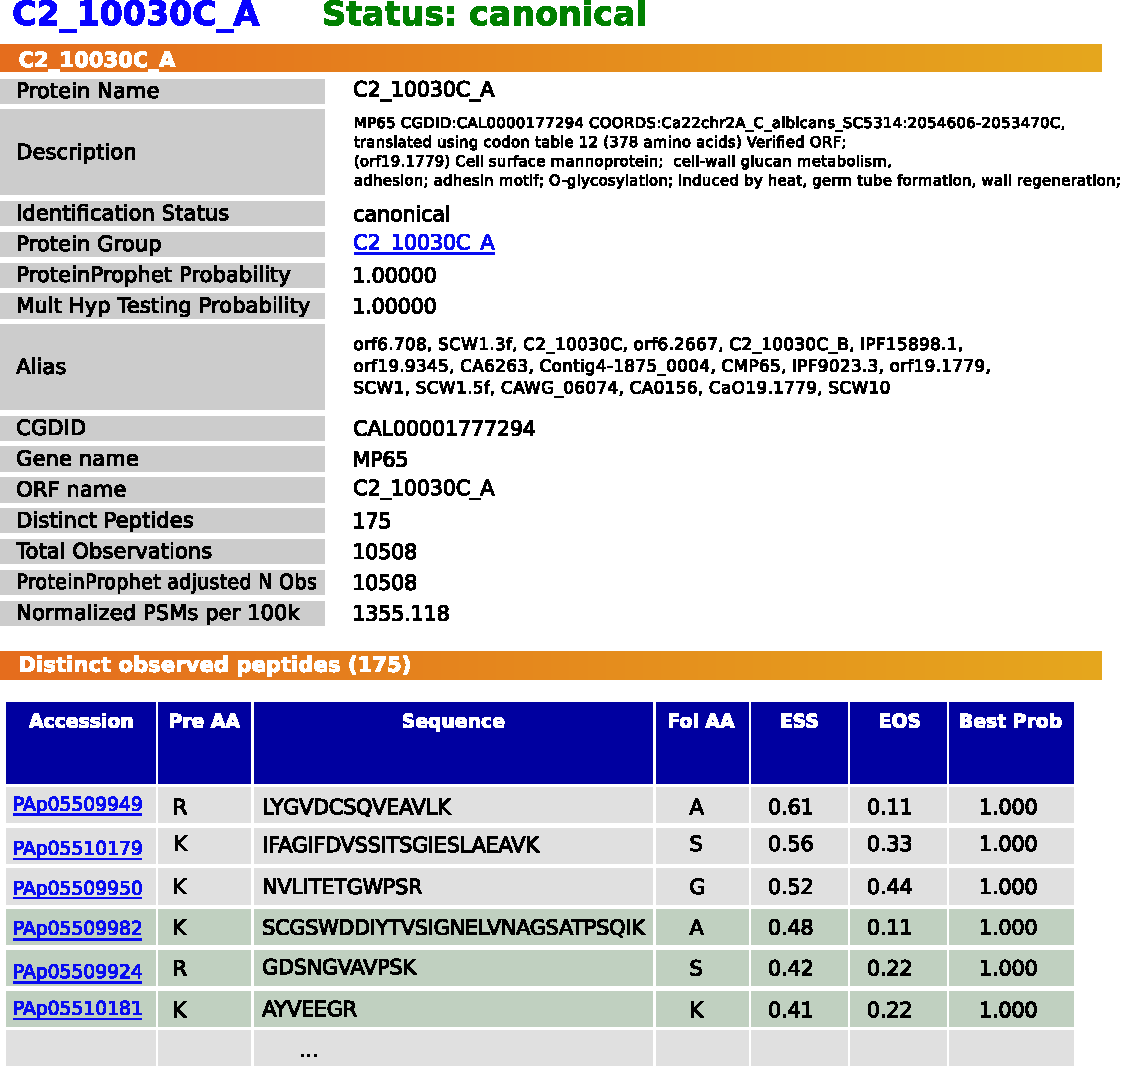
\includegraphics[width=0.90\textwidth]{Imagenes/Vectorial/PeptideAtlasMP65}
\caption*{Figura 2.2: Informaci�n b�sica para Mp65p, una manoprote�na de pared, inmunog�nica, implicada en adhesi�n,
\citep{LaValle2000, Sandini2011} y p�ptidos observados en PeptideAtlas. %
El par�metro EOS (\emph{Empirical Observability Score}) estima c�mo de probable es que si una prote�na
es detectada lo sea por medio de ese p�ptido y no otro.
Los p�ptidos se presentan ordenados por el par�metro ESS (\emph{Empirical Suitability Score}) %
que combina la informaci�n de la probabilidad del p�ptido, su observabilidad (EOS) y el n�mero de veces que es detectado.
Adem�s se muestra si un p�ptido presenta sitios de corte no efectuado o si su secuencia es mapeable con m�ltiples sitios en el genoma.
Toda esta informaci�n puede ser de gran utilidad para seleccionar p�ptidos proteot�picos candidatos para un ensayo de prote�mica dirigida SRM o MRM.}
\end{center}
\end{figure}
\addcontentsline{lof}{figure}{2.2. Informaci�n b�sica para Mp65p \newline y p�ptidos observados en \mbox{PeptideAtlas}}




\medskip

El PeptideAtlas creado proporciona una visi�n general representativa del proteoma
de \textit{C. albicans} como demuestra la semejanza entre la distribuci�n
de frecuencias de t�rminos GO en el subconjunto de prote�nas detectadas y
la distribuci�n correspondiente para todo el genoma. Y sin embargo,
a�n ser� posible en el futuro crear nuevas versiones mejoradas del atlas 
en las que se reanalicen otros resultados depositados en ProteomeXchange \citep{Vizcaino2014},
resultados de estudios enfocados a detectar prote�nas elusivas
expresadas en circunstancias muy particulares, prote�nas dif�ciles de extraer,
o traducidas en muy escasa cantidad.
Adem�s, mejoras en los elementos del \textit{software} que integran el flujo
de an�lisis, o en la base de datos de secuencias tambi�n contribuir�n a motivar
la construcci�n de futuras versiones de este PeptideAtlas.

\medskip

Por �ltimo, y para favorecer la comunicaci�n e interconexi�n entre ambos
recursos, CGD y PeptideAtlas, se ha contactado con los desarrolladores 
e impulsores de CGD proporcion�ndoles un formato de enlace para que, a trav�s
de la informaci�n en la pesta�a \textit{prote�na} en CGD, se pueda
acceder a los datos correspondientes a la identificaci�n en PeptideAtlas
para aquellas prote�nas para las que existan estos datos.


\medskip

En definitiva, las herramientas bioinform�ticas descritas en esta tesis contribuyen
a ampliar y mejorar el cat�logo existente de p�ptidos y prote�nas detectadas en estudios
de prote�mica que utilizan el modelo de \textit{C. albicans} bajo distintas condiciones.
Estas herramientas descritas, Proteopathogen y PeptideAtlas, ocupan nichos diferentes
pero complementarios en este objetivo. PeptideAtlas cuenta con su propio flujo de an�lisis y validaci�n estad�stica de los resultados
y proporciona una base de datos y una interfaz web para visualizar los resultados de identificaciones.
Es actualmente el cat�logo m�s completo del proteoma de \textit{C. albicans},
cuenta con una contrastada robustez y fiabilidad y forma parte de un proyecto global de reconocido prestigio.
Proteopathogen, una base de datos y aplicacion web basada en el est�ndar mzIdentML,
es vers�til y completamente independiente
del procesamiento experimental y computacional que origina los resultados.
Permite integrar r�pidamente resultados de identificaciones de or�genes diversos 
independientemente del post-procesamiento y an�lisis estad�stico empleado ya sea
el proporcionado por el flujo de trabajo TPP caracter�stico de PeptideAtlas u otro.%y %al estar alojada en un servidor accesible







 %Este es un capitulo especial, igual que Introduccion

%---------------------------------------------------------------------
%
%                          Parte Conclusiones
%
%---------------------------------------------------------------------
%
% Copyright 2009 Marco Antonio Gomez-Martin, Pedro Pablo Gomez-Martin
%
% This file belongs to the TeXiS manual, a LaTeX template for writting
% Thesis and other documents. The complete last TeXiS package can
% be obtained from http://gaia.fdi.ucm.es/projects/texis/
%
% Although the TeXiS template itself is distributed under the 
% conditions of the LaTeX Project Public License
% (http://www.latex-project.org/lppl.txt), the manual content
% uses the CC-BY-SA license that stays that you are free:
%
%    - to share & to copy, distribute and transmit the work
%    - to remix and to adapt the work
%
% under the following conditions:
%
%    - Attribution: you must attribute the work in the manner
%      specified by the author or licensor (but not in any way that
%      suggests that they endorse you or your use of the work).
%    - Share Alike: if you alter, transform, or build upon this
%      work, you may distribute the resulting work only under the
%      same, similar or a compatible license.
%
% The complete license is available in
% http://creativecommons.org/licenses/by-sa/3.0/legalcode
%
%---------------------------------------------------------------------

% Definici�n de la primera parte del manual

\partTitle{\sc{Conclusiones}}


%\partDesc{Esta es una introducci�n general a todos los cap�tulos (papers) de la tesis.
%  Por eso tiene la estructura de una "parte" de la tesis.
%  Esta "parte" no tendr� cap�tulos sino secciones y subsecciones.
%  La segunda "parte" de la tesis es la que contiene los cap�tulos (papers)
%  La tercera ser� una discusi�n general a todos los capitulos de la segunda parte }

%En realidad aqui no pongo nada, es una hoja en la que solo pone Introduccion

%\partBackText{En realidad la divisi�n por partes del manual no aporta
%  demasiado al lector; se ha dividido en varias partes debido a que,
%  en la pr�ctica, el c�digo de este manual sirve como ejemplo de uso
%  de \texis.

%  En un contexto distinto, es posible que un manual de este tipo no
%  habr�a tenido estas partes as� de diferenciadas.}

\makepart


 %Conclusiones
%---------------------------------------------------------------------
%
%                         Conclusiones
%---------------------------------------------------------------------

\chapter*{Conclusiones}
%mirar problema con fancyheader y secciones no numeradas, pagina 21-22 del manual
%\fancyhead[RO,LE]{\sc{Conclusiones}}
\addcontentsline{toc}{chapter}{Conclusiones}



\begin{enumerate}

\item La base de datos y aplicaci�n web Proteopathogen
ha demostrado ser una herramienta de gran utilidad para la visualizaci�n
y an�lisis de resultados de prote�mica en experimentos que usan 
\textit{Candida albicans} como organismo modelo de estudio de hongos pat�genos.

\item La adopci�n del est�ndar mzIdentML como formato de origen para
incorporar nuevos datos en Proteopathogen asegura la estabilidad y futuro
de este proyecto facilitando la incorporaci�n de resultados procedentes 
de nuevos experimentos.

\item El PeptideAtlas de \textit{Candida albicans} desarrollado
supone la caracterizaci�n m�s exahustiva del proteoma de este organismo.
y es el recurso m�s completo y fiable disponible p�blicamente.



\end{enumerate}
 %Este es un capitulo especial, igual que Introduccion


\backmatter

%
% Bibliografía
%

%---------------------------------------------------------------------
%
%                      configBibliografia.tex
%
%---------------------------------------------------------------------
%
% bibliografia.tex
% Copyright 2009 Marco Antonio Gomez-Martin, Pedro Pablo Gomez-Martin
%
% This file belongs to the TeXiS manual, a LaTeX template for writting
% Thesis and other documents. The complete last TeXiS package can
% be obtained from http://gaia.fdi.ucm.es/projects/texis/
%
% Although the TeXiS template itself is distributed under the 
% conditions of the LaTeX Project Public License
% (http://www.latex-project.org/lppl.txt), the manual content
% uses the CC-BY-SA license that stays that you are free:
%
%    - to share & to copy, distribute and transmit the work
%    - to remix and to adapt the work
%
% under the following conditions:
%
%    - Attribution: you must attribute the work in the manner
%      specified by the author or licensor (but not in any way that
%      suggests that they endorse you or your use of the work).
%    - Share Alike: if you alter, transform, or build upon this
%      work, you may distribute the resulting work only under the
%      same, similar or a compatible license.
%
% The complete license is available in
% http://creativecommons.org/licenses/by-sa/3.0/legalcode
%
%---------------------------------------------------------------------
%
% Fichero  que  configura  los  par�metros  de  la  generaci�n  de  la
% bibliograf�a.  Existen dos  par�metros configurables:  los ficheros
% .bib que se utilizan y la frase c�lebre que aparece justo antes de la
% primera referencia.
%
%---------------------------------------------------------------------


%
%\restauraCabecera{}
\cabeceraEspecial{Bibliograf�a}
\fancyhead[RO,LE]{\sc{Bibliograf�a}}
%\fancyhead[RO,LE]{BIBLIOGRAF�A}



%%%%%%%%%%%%%%%%%%%%%%%%%%%%%%%%%%%%%%%%%%%%%%%%%%%%%%%%%%%%%%%%%%%%%%
% Definici�n de los ficheros .bib utilizados:
% \setBibFiles{<lista ficheros sin extension, separados por comas>}
% Nota:
% Es IMPORTANTE que los ficheros est�n en la misma l�nea que
% el comando \setBibFiles. Si se desea utilizar varias l�neas,
% terminarlas con una apertura de comentario.
% Nota Vital: a�ado aqui library: library.bib es la biblografia de Mendeley
%%%%%%%%%%%%%%%%%%%%%%%%%%%%%%%%%%%%%%%%%%%%%%%%%%%%%%%%%%%%%%%%%%%%%%

\setBibFiles{library}

%%%%%%%%%%%%%%%%%%%%%%%%%%%%%%%%%%%%%%%%%%%%%%%%%%%%%%%%%%%%%%%%%%%%%%
% Definici�n de la frase c�lebre para el cap�tulo de la
% bibliograf�a. Dentro normalmente se querr� hacer uso del entorno
% \begin{FraseCelebre}, que contendr� a su vez otros dos entornos,
% un \begin{Frase} y un \begin{Fuente}.
%
% Nota:
% Si no se quiere cita, se puede eliminar su definici�n (en la
% macro setCitaBibliografia{} ).
%%%%%%%%%%%%%%%%%%%%%%%%%%%%%%%%%%%%%%%%%%%%%%%%%%%%%%%%%%%%%%%%%%%%%%
%


\setCitaBibliografia{
\begin{FraseCelebre}
\begin{Frase}
  ..y as�, del poco dormir y del mucho leer, se le sec� el celebro de
  manera que vino a perder el juicio.
\end{Frase}

\hfill

\begin{Fuente}

  \hfill{\emph{Primera parte de El Ingenioso Caballero Don Quijote de la Mancha}}

  \hfill{\mbox{\emph{Miguel de Cervantes Saavedra}}}

\end{Fuente}
\end{FraseCelebre}
}



%
%\setCitaBibliografia{
%\begin{FraseCelebre}
%\begin{Frase}
%Siempre imagin� que el Para�so ser�a alg�n tipo de biblioteca
%Que otros se jacten de las p�ginas que han escrito; a mi me enorgullecen las que he le�do
%\end{Frase}
%\begin{Fuente}
   %Jorge Luis Borges
%\end{Fuente}
%\end{FraseCelebre}
%}
%





%%
%% Creamos la bibliografia
%%
\makeBib

% Variable local para emacs, para  que encuentre el fichero maestro de
% compilaci�n y funcionen mejor algunas teclas r�pidas de AucTeX

%%%
%%% Local Variables:
%%% mode: latex
%%% TeX-master: "../Tesis.tex"
%%% End:




%
% Índice de palabras
%

% Sólo  la   generamos  si  está   declarada  \generaindice.  Consulta
% TeXiS.sty para más información.

% En realidad, el soporte para la generación de índices de palabras
% en TeXiS no está documentada en el manual, porque no ha sido usada
% "en producción". Por tanto, el fichero que genera el índice
% *no* se incluye aquí (está comentado). Consulta la documentación
% en TeXiS_pream.tex para más información.
\ifx\generaindice\undefined
\else
%%---------------------------------------------------------------------
%
%                        TeXiS_indice.tex
%
%---------------------------------------------------------------------
%
% TeXiS_indice.tex
% Copyright 2009 Marco Antonio Gomez-Martin, Pedro Pablo Gomez-Martin
%
% This file belongs to TeXiS, a LaTeX template for writting
% Thesis and other documents. The complete last TeXiS package can
% be obtained from http://gaia.fdi.ucm.es/projects/texis/
%
% This work may be distributed and/or modified under the
% conditions of the LaTeX Project Public License, either version 1.3
% of this license or (at your option) any later version.
% The latest version of this license is in
%   http://www.latex-project.org/lppl.txt
% and version 1.3 or later is part of all distributions of LaTeX
% version 2005/12/01 or later.
%
% This work has the LPPL maintenance status `maintained'.
% 
% The Current Maintainers of this work are Marco Antonio Gomez-Martin
% and Pedro Pablo Gomez-Martin
%
%---------------------------------------------------------------------
%
% Contiene  los  comandos  para  generar  el �ndice  de  palabras  del
% documento.
%
%---------------------------------------------------------------------
%
% NOTA IMPORTANTE: el  soporte en TeXiS para el  �ndice de palabras es
% embrionario, y  de hecho  ni siquiera se  describe en el  manual. Se
% proporciona  una infraestructura  b�sica (sin  terminar)  para ello,
% pero  no ha  sido usada  "en producci�n".  De hecho,  a pesar  de la
% existencia de  este fichero, *no* se incluye  en Tesis.tex. Consulta
% la documentaci�n en TeXiS_pream.tex para m�s informaci�n.
%
%---------------------------------------------------------------------


% Si se  va a generar  la tabla de  contenidos (el �ndice  habitual) y
% tambi�n vamos a  generar el �ndice de palabras  (ambas decisiones se
% toman en  funci�n de  la definici�n  o no de  un par  de constantes,
% puedes consultar modo.tex para m�s informaci�n), entonces metemos en
% la tabla de contenidos una  entrada para marcar la p�gina donde est�
% el �ndice de palabras.

\ifx\generatoc\undefined
\else
   \addcontentsline{toc}{chapter}{\indexname}
\fi

% Generamos el �ndice
\printindex

% Variable local para emacs, para  que encuentre el fichero maestro de
% compilaci�n y funcionen mejor algunas teclas r�pidas de AucTeX

%%%
%%% Local Variables:
%%% mode: latex
%%% TeX-master: "./tesis.tex"
%%% End:

\fi

%
% Lista de acrónimos
%

% Sólo  lo  generamos  si  está declarada  \generaacronimos.  Consulta
% TeXiS.sty para más información.


\ifx\generaacronimos\undefined
\else
%---------------------------------------------------------------------
%
%                        TeXiS_acron.tex
%
%---------------------------------------------------------------------
%
% TeXiS_acron.tex
% Copyright 2009 Marco Antonio Gomez-Martin, Pedro Pablo Gomez-Martin
%
% This file belongs to TeXiS, a LaTeX template for writting
% Thesis and other documents. The complete last TeXiS package can
% be obtained from http://gaia.fdi.ucm.es/projects/texis/
%
% This work may be distributed and/or modified under the
% conditions of the LaTeX Project Public License, either version 1.3
% of this license or (at your option) any later version.
% The latest version of this license is in
%   http://www.latex-project.org/lppl.txt
% and version 1.3 or later is part of all distributions of LaTeX
% version 2005/12/01 or later.
%
% This work has the LPPL maintenance status `maintained'.
% 
% The Current Maintainers of this work are Marco Antonio Gomez-Martin
% and Pedro Pablo Gomez-Martin
%
%---------------------------------------------------------------------
%
% Contiene  los  comandos  para  generar  el listado de acr�nimos
% documento.
%
%---------------------------------------------------------------------
%
% NOTA IMPORTANTE:  para que la  generaci�n de acr�nimos  funcione, al
% menos  debe  existir  un  acr�nimo   en  el  documento.  Si  no,  la
% compilaci�n  del   fichero  LaTeX  falla  con   un  error  "extra�o"
% (indicando  que  quiz�  falte  un \item).   Consulta  el  comentario
% referente al paquete glosstex en TeXiS_pream.tex.
%
%---------------------------------------------------------------------



% Redefinimos a espa�ol  el t�tulo de la lista  de acr�nimos (Babel no
% lo hace por nosotros esta vez)

\def\listacronymname{Lista de acr�nimos}


% Para el glosario:
% \def\glosarryname{Glosario}

% Si se  va a generar  la tabla de  contenidos (el �ndice  habitual)F y
% tambi�n vamos a  generar la lista de acr�nimos  (ambas decisiones se
% toman en  funci�n de  la definici�n  o no de  un par  de constantes,
% puedes consultar config.tex  para m�s informaci�n), entonces metemos
% en la  tabla de contenidos una  entrada para marcar  la p�gina donde
% est� el �ndice de palabras.

%comentar para poner/quitar "Lista de acr�nimos en el TOC"
\ifx\generatoc\undefined
\else
   \addcontentsline{toc}{chapter}{\listacronymname}
\fi

%




% Generamos la lista de acr�nimos (en realidad el �ndice asociado a la
% lista "acr" de GlossTeX)

\cabeceraEspecial
\fancyhead
\printglosstex(acr)

% Variable local para emacs, para  que encuentre el fichero maestro de
% compilaci�n y funcionen mejor algunas teclas r�pidas de AucTeX

%%%
%%% Local Variables:
%%% mode: latex
%%% TeX-master: "../Tesis.tex"
%%% End:

\fi

%
% Final
%
%---------------------------------------------------------------------
%
%                      fin.tex
%
%---------------------------------------------------------------------
%
% fin.tex
% Copyright 2009 Marco Antonio Gomez-Martin, Pedro Pablo Gomez-Martin
%
% This file belongs to the TeXiS manual, a LaTeX template for writting
% Thesis and other documents. The complete last TeXiS package can
% be obtained from http://gaia.fdi.ucm.es/projects/texis/
%
% Although the TeXiS template itself is distributed under the 
% conditions of the LaTeX Project Public License
% (http://www.latex-project.org/lppl.txt), the manual content
% uses the CC-BY-SA license that stays that you are free:
%
%    - to share & to copy, distribute and transmit the work
%    - to remix and to adapt the work
%
% under the following conditions:
%
%    - Attribution: you must attribute the work in the manner
%      specified by the author or licensor (but not in any way that
%      suggests that they endorse you or your use of the work).
%    - Share Alike: if you alter, transform, or build upon this
%      work, you may distribute the resulting work only under the
%      same, similar or a compatible license.
%
% The complete license is available in
% http://creativecommons.org/licenses/by-sa/3.0/legalcode
%
%---------------------------------------------------------------------
%
% Contiene la �ltima p�gina
%
%---------------------------------------------------------------------


% Ponemos el marcador en el PDF al nivel adecuado, dependiendo
% de su hubo partes en el documento o no (si las hay, queremos
% que aparezca "al mismo nivel" que las partes.
\ifpdf
\ifx\tienePartesTeXiS\undefined
   \pdfbookmark[0]{Fin}{fin}
\else
   \pdfbookmark[-1]{Fin}{fin}
\fi
\fi

\thispagestyle{empty}\mbox{}

\vspace*{4cm}

\small

\hfill \emph{--�Qu� te parece desto, Sancho? -- Dijo Don Quijote --}

\hfill \emph{Bien podr�n los encantadores quitarme la ventura,}

\hfill \emph{pero el esfuerzo y el �nimo, ser� imposible.}

\hfill 

\hfill \emph{Segunda parte de El Ingenioso Caballero} 

\hfill \emph{Don Quijote de la Mancha}

\hfill \emph{Miguel de Cervantes Saavedra}

\vfill%space*{4cm}

\hfill \emph{--Buena est� -- dijo Sancho --; f�rmela vuestra merced.}

\hfill \emph{--No es menester firmarla -- dijo Don Quijote--,}

\hfill \emph{sino solamente poner mi r�brica.}

\hfill 

\hfill \emph{Primera parte de El Ingenioso Caballero} 

\hfill \emph{Don Quijote de la Mancha}

\hfill \emph{Miguel de Cervantes Saavedra}


\newpage
\thispagestyle{empty}\mbox{}

\newpage

% Variable local para emacs, para  que encuentre el fichero maestro de
% compilaci�n y funcionen mejor algunas teclas r�pidas de AucTeX

%%%
%%% Local Variables:
%%% mode: latex
%%% TeX-master: "../Tesis.tex"
%%% End:


\end{document}
